% ---------------------------------------------------------------------------
% glycolysis.tex --- KEGG M00001 end to end: topology, exact structure, the
% returned firing certificate, and every recorded token marking.
%
% Source fragment: loaded directly by main.tex.
%
% Every number comes from Figure/glycolysis_analysis.tex, regenerated by
% Figure/glycolysis_analysis.py from the cached module.
%
% Top panels show the reduced pathway and exact structural diagnostics.
% The full-width lower panel is generated from the complete recorded trajectory.
% ---------------------------------------------------------------------------
% Resolve the shared style and generated analysis macros from the manuscript
% root.
\IfFileExists{synstyle.tex}{% ---------------------------------------------------------------------------
% synstyle.tex --- shared look for every TikZ figure of the SynKit CRN paper.
%
% Input it from a figure file:
%     \IfFileExists{synstyle.tex}{% ---------------------------------------------------------------------------
% synstyle.tex --- shared look for every TikZ figure of the SynKit CRN paper.
%
% Input it from a figure file:
%     \IfFileExists{synstyle.tex}{% ---------------------------------------------------------------------------
% synstyle.tex --- shared look for every TikZ figure of the SynKit CRN paper.
%
% Input it from a figure file:
%     \IfFileExists{synstyle.tex}{\input{synstyle}}{\input{Figure/synstyle}}
% so that the figure compiles both from Figure/ and from the paper root.
%
% The visual vocabulary follows ../../../../Style/style.tex: the
% colour-blind-safe Okabe--Ito accents, quiet neutral rules and wash, circular
% panel badges, and a compact technical type scale are shared by the companion
% papers.  Semantic aliases below keep the CRN meaning explicit.
%
% DESIGN CONTRACT -----------------------------------------------------------
% 1. Geometry.  Every figure is laid out on a canvas exactly \scW wide (the
%    sn-jnl text width, 372 pt) and is included unscaled, so one point of type
%    is the same physical size in all five figures.  Open each picture with
%    \scCanvas{<height in cm>} to pin the bounding box.
% 2. Colour is semantic, never decorative.  Four roles only:
%       scAccent (green)       structure, the normal/expected path
%       scMark   (orange)      catalyst, certificate, or highlight
%       scAlert  (vermillion)  failure, violation, or uncovered set
%       scRef    (blue)        secondary or reference series
%    A panel gets at most one accent.  Titles are always ink; panel identity
%    is also encoded by a letter inside a circular badge, not by colour alone.
% 3. Type scale.  Three sizes, no others, and nothing below 6 pt:
%       \scTitle (7 pt bold)  panel titles
%       \scBody  (6.5 pt)     labels, values, in-figure prose
%       \scSmall (6 pt)       units, footnotes, dense graph labels
% ---------------------------------------------------------------------------
% Load guard.  The paper inputs every figure source inline, so this file is
% reached once per figure; without the guard the second \newlength below
% would abort the run.
\ifdefined\SynKitStyleLoaded\endinput\fi
\newcommand{\SynKitStyleLoaded}{}

% Load in the document preamble. XeLaTeX/LuaLaTeX and an installed Arial
% family are required; fontspec reports an error instead of substituting.
\RequirePackage[no-math]{fontspec}
\newfontfamily\scArial{Arial}[NFSSFamily=scArial,Ligatures=TeX]
% Keep manuscript mathematics unchanged; select Arial letters and numerals
% only inside figures. TeX supplies specialist mathematical symbols.
\RequirePackage[subdued,italic]{mathastext}
\MTDeclareVersion{synarial}{TU}{scArial}{m}{n}
\SetMathAlphabet{\Mathsf}{synarial}{TU}{scArial}{m}{n}
\SetMathAlphabet{\Mathtt}{synarial}{TU}{scArial}{m}{n}

\usetikzlibrary{positioning,calc,fit,backgrounds,arrows.meta,shapes.geometric,
                shapes.misc,decorations.pathreplacing,patterns,math}

% --- canvas ---------------------------------------------------------------
% 372 pt text width minus the 1 pt standalone border on each side.
\newlength{\scW}\setlength{\scW}{13.0326cm}
\providecommand{\scWnum}{13.0326}
% \scCanvas{<height>} pins the picture to the full text width, y running down
% from 0, so every figure shares one coordinate convention.  It *sets* the
% bounding box rather than contributing to it, so the emitted page is exactly
% the text width and every figure is included at 1:1 -- otherwise a stray
% invisible extent (pgfplots reserves a little around an axis) rescales one
% figure relative to the others and the same \scSmall prints at two sizes.
% Anything drawn outside the canvas is therefore cropped: keep content inside,
% and check with
%     \providecommand{\scCanvas}[1]{\path[draw=red] (0,0) rectangle (\scWnum,-#1);}
\providecommand{\scCanvas}[1]{%
  \path[use as bounding box] (0,0) rectangle (\scWnum,-#1);}

% --- palette --------------------------------------------------------------
% Canonical companion-paper values (../../../../Style/style.tex).
\definecolor{npgOrange}{HTML}{E69F00}
\definecolor{npgSky}{HTML}{56B4E9}
\definecolor{npgGreen}{HTML}{009E73}
\definecolor{npgYellow}{HTML}{F0E442}
\definecolor{npgBlue}{HTML}{0072B2}
\definecolor{npgVermillion}{HTML}{E64B35}
\definecolor{npgPurple}{HTML}{CC79A7}
\definecolor{figInk}{HTML}{1A1A1A}
\definecolor{figMuted}{HTML}{666666}
\definecolor{figHair}{HTML}{D9D9D9}
\definecolor{figWash}{HTML}{F7F7F7}

\colorlet{scInk}{figInk}              % primary text
\colorlet{scInkM}{figMuted}           % secondary text
\colorlet{scPaper}{figWash}           % quiet cards and note strips
\colorlet{scSpF}{npgSky!12}           % species fill
\colorlet{scSpE}{npgBlue}             % species edge
\colorlet{scRxF}{npgOrange!12}        % reaction fill
\colorlet{scRxE}{npgOrange!88!black}  % reaction edge
\colorlet{scReac}{npgBlue!78!black}   % reactant edge
\colorlet{scProd}{npgGreen!82!black}  % product edge
\colorlet{scHiF}{npgOrange!13}        % highlight fill
\colorlet{scHiE}{npgOrange!82!black}  % highlight edge
% Stage / accent tints.  stDE remains available for the fifth plot series.
\colorlet{stAF}{npgGreen!9}\colorlet{stAE}{npgGreen}
\colorlet{stBF}{npgOrange!11}\colorlet{stBE}{npgOrange}
\colorlet{stCF}{npgBlue!9}\colorlet{stCE}{npgBlue}
\colorlet{stDF}{npgPurple!10}\colorlet{stDE}{npgPurple!85!black}
\colorlet{stEF}{npgVermillion!9}\colorlet{stEE}{npgVermillion}

% Semantic aliases.  Figures should speak in these, not in stAE/stBE/...
\colorlet{scAccent}{stAE}\colorlet{scAccentF}{stAF}   % structure / normal
\colorlet{scMark}{stBE}\colorlet{scMarkF}{stBF}       % highlight / certificate
\colorlet{scRef}{stCE}\colorlet{scRefF}{stCF}         % secondary series
\colorlet{scAlert}{stEE}\colorlet{scAlertF}{stEF}     % failure / violation
\colorlet{scRule}{figHair}                            % card and axis hairlines
\colorlet{scRuleL}{figHair!55}                        % grid, dividers

% --- text styles ----------------------------------------------------------
% Three sizes, fixed in points so they do not drift with the document class.
% Arial is shared by labels, headings, panel badges, and chemistry labels.
\providecommand{\scTitle}{\scArial\fontsize{7}{8.4}\selectfont\bfseries\color{scInk}}
\providecommand{\scBody}{\scArial\fontsize{6.5}{7.8}\selectfont\color{scInkM}}
\providecommand{\scSmall}{\scArial\fontsize{6}{7.2}\selectfont\color{scInkM}}
\providecommand{\scSub}[1]{{\scSmall\itshape #1}}
\providecommand{\scPanel}[1]{{\scTitle(#1)}}
% Numerals that carry a result: ink, not colour, so the eye reads the value.
\providecommand{\scNum}{\scArial\fontsize{10}{11}\selectfont\bfseries\color{scInk}}

% --- shared TikZ styles ---------------------------------------------------
\tikzset{
  % text never hyphenates inside a figure
  every node/.append style={execute at begin node={%
      \hyphenpenalty=10000 \exhyphenpenalty=10000 \hbadness=10000 }},
  syn/.style={font=\scArial,color=scInk,
              execute at begin picture={\MTversion*{synarial}},
              >={Stealth[round,length=2.4mm,width=1.9mm]}},
  % containers ------------------------------------------------------------
  % One card chrome for the whole paper: white, 3 pt radius, one hairline.
  panel/.style={rounded corners=2.5pt,fill=none,draw=scRule,line width=0.45pt},
  card/.style={rounded corners=2.2pt,fill=scPaper,draw=scRule,line width=0.45pt,
               inner sep=5pt,align=left,anchor=north west},
  % a quiet strip for a panel's closing fact
  note/.style={rounded corners=2.5pt,fill=scPaper,draw=scRuleL,line width=0.4pt,
               inner xsep=6pt,inner ysep=3.5pt,align=left,font=\scSmall},
  % small labelled value pill
  chip/.style={rounded corners=2pt,fill=scPaper,draw=scRule,line width=0.4pt,
               inner xsep=4pt,inner ysep=2pt,font=\scSmall},
  % Circular letter badge: the same accessible panel marker used in Style/*.
  hbullet/.style={circle,fill=scInk,text=white,draw=none,
                  font=\scArial\fontsize{6}{6}\selectfont\bfseries,
                  minimum size=4.2mm,inner sep=0pt},
  ctag/.style={font=\scTitle,anchor=north west,text=scInk},
  % CRN primitives --------------------------------------------------------
  species/.style={rounded rectangle,fill=scSpF,draw=scSpE,line width=0.45pt,
                  inner xsep=2.4pt,inner ysep=1.6pt,font=\scSmall,
                  text=scInk,minimum height=3.6mm},
  cofactor/.style={species,fill=scRefF,draw=scRef},
  catalyst/.style={species,fill=scHiF,draw=scHiE},
  rxn/.style={rectangle,fill=scRxF,draw=scRxE,line width=0.45pt,
              inner sep=1.2pt,font=\scSmall,text=scInk,
              minimum width=3.0mm,minimum height=3.0mm},
  place/.style={circle,fill=scSpF,draw=scSpE,line width=0.45pt,
                minimum size=4.0mm,inner sep=0pt},
  trans/.style={rectangle,fill=scRxE,draw=scRxE,minimum width=1.1mm,
                minimum height=3.6mm,inner sep=0pt},
  token/.style={circle,fill=scInk,minimum size=1.1mm,inner sep=0pt},
  % edges -----------------------------------------------------------------
  reac/.style={->,line width=0.5pt,draw=scReac,shorten >=0.8pt,shorten <=0.8pt},
  prod/.style={->,line width=0.5pt,draw=scProd,shorten >=0.8pt,shorten <=0.8pt},
  cat/.style={->,line width=0.5pt,draw=scHiE,shorten >=0.8pt,shorten <=0.8pt},
  flow/.style={-{Stealth[round,length=2.2mm,width=1.8mm]},line width=1.1pt,
               draw=scInkM!45},
  flab/.style={font=\scSmall,text=scInkM,inner sep=2pt},
  stoi/.style={font=\scSmall,text=scInkM,inner sep=0.8pt},
  % verdict marks: shape carries the meaning, colour only reinforces it
  vpass/.style={circle,fill=scAccentF,draw=scAccent,text=scAccent,
                font=\fontsize{6}{6}\selectfont\bfseries,
                minimum size=3.2mm,inner sep=0pt},
  vfail/.style={circle,fill=scAlertF,draw=scAlert,text=scAlert,
                font=\fontsize{6}{6}\selectfont\bfseries,
                minimum size=3.2mm,inner sep=0pt},
  callout/.style={font=\scSmall,text=scInkM,align=left},
}

% \scHead[<badge colour>]{<anchor coord>}{<letter>}{<title>}{<subtitle or empty>}
% One header treatment for every panel in the paper.
\providecommand{\scHead}[5][scInk]{%
  \node[hbullet,fill=#1,anchor=north west] (scbadge#3) at ($#2+(0,-0.015)$)
    {\MakeUppercase{#3}};
  \node[ctag,anchor=west] at ($(scbadge#3.east)+(0.14,0)$) {#4};
  \ifx\relax#5\relax\else
    \node[anchor=north west,font=\scSmall,text=scInkM]
      at ($#2+(0.56,-0.245)$) {#5};
  \fi}

% --- shared pgfplots look (only if the figure loaded pgfplots) ------------
\ifdefined\pgfplotsset
  \pgfplotsset{compat=1.18}
  \pgfplotsset{
    synaxis/.style={
      scale only axis,
      tick align=outside, tick pos=left,
      axis line style={draw=scInkM!55,line width=0.4pt},
      % One grid, on the value axis only.  No minor grid: at these sizes it
      % turns the plot frame into a grey wash.
      ymajorgrids=true, xmajorgrids=false,
      major grid style={draw=scRuleL,line width=0.3pt},
      major tick length=1.6pt,
      label style={font=\scBody,color=scInk},
      tick label style={font=\scSmall,color=scInkM},
      legend style={font=\scSmall,draw=none,fill=none,inner sep=1pt,
                    row sep=0.4pt,legend columns=1},
      legend cell align=left,
      every axis plot/.append style={line width=0.7pt,mark size=1.2pt},
    },
  }
\fi
}{% ---------------------------------------------------------------------------
% synstyle.tex --- shared look for every TikZ figure of the SynKit CRN paper.
%
% Input it from a figure file:
%     \IfFileExists{synstyle.tex}{\input{synstyle}}{\input{Figure/synstyle}}
% so that the figure compiles both from Figure/ and from the paper root.
%
% The visual vocabulary follows ../../../../Style/style.tex: the
% colour-blind-safe Okabe--Ito accents, quiet neutral rules and wash, circular
% panel badges, and a compact technical type scale are shared by the companion
% papers.  Semantic aliases below keep the CRN meaning explicit.
%
% DESIGN CONTRACT -----------------------------------------------------------
% 1. Geometry.  Every figure is laid out on a canvas exactly \scW wide (the
%    sn-jnl text width, 372 pt) and is included unscaled, so one point of type
%    is the same physical size in all five figures.  Open each picture with
%    \scCanvas{<height in cm>} to pin the bounding box.
% 2. Colour is semantic, never decorative.  Four roles only:
%       scAccent (green)       structure, the normal/expected path
%       scMark   (orange)      catalyst, certificate, or highlight
%       scAlert  (vermillion)  failure, violation, or uncovered set
%       scRef    (blue)        secondary or reference series
%    A panel gets at most one accent.  Titles are always ink; panel identity
%    is also encoded by a letter inside a circular badge, not by colour alone.
% 3. Type scale.  Three sizes, no others, and nothing below 6 pt:
%       \scTitle (7 pt bold)  panel titles
%       \scBody  (6.5 pt)     labels, values, in-figure prose
%       \scSmall (6 pt)       units, footnotes, dense graph labels
% ---------------------------------------------------------------------------
% Load guard.  The paper inputs every figure source inline, so this file is
% reached once per figure; without the guard the second \newlength below
% would abort the run.
\ifdefined\SynKitStyleLoaded\endinput\fi
\newcommand{\SynKitStyleLoaded}{}

% Load in the document preamble. XeLaTeX/LuaLaTeX and an installed Arial
% family are required; fontspec reports an error instead of substituting.
\RequirePackage[no-math]{fontspec}
\newfontfamily\scArial{Arial}[NFSSFamily=scArial,Ligatures=TeX]
% Keep manuscript mathematics unchanged; select Arial letters and numerals
% only inside figures. TeX supplies specialist mathematical symbols.
\RequirePackage[subdued,italic]{mathastext}
\MTDeclareVersion{synarial}{TU}{scArial}{m}{n}
\SetMathAlphabet{\Mathsf}{synarial}{TU}{scArial}{m}{n}
\SetMathAlphabet{\Mathtt}{synarial}{TU}{scArial}{m}{n}

\usetikzlibrary{positioning,calc,fit,backgrounds,arrows.meta,shapes.geometric,
                shapes.misc,decorations.pathreplacing,patterns,math}

% --- canvas ---------------------------------------------------------------
% 372 pt text width minus the 1 pt standalone border on each side.
\newlength{\scW}\setlength{\scW}{13.0326cm}
\providecommand{\scWnum}{13.0326}
% \scCanvas{<height>} pins the picture to the full text width, y running down
% from 0, so every figure shares one coordinate convention.  It *sets* the
% bounding box rather than contributing to it, so the emitted page is exactly
% the text width and every figure is included at 1:1 -- otherwise a stray
% invisible extent (pgfplots reserves a little around an axis) rescales one
% figure relative to the others and the same \scSmall prints at two sizes.
% Anything drawn outside the canvas is therefore cropped: keep content inside,
% and check with
%     \providecommand{\scCanvas}[1]{\path[draw=red] (0,0) rectangle (\scWnum,-#1);}
\providecommand{\scCanvas}[1]{%
  \path[use as bounding box] (0,0) rectangle (\scWnum,-#1);}

% --- palette --------------------------------------------------------------
% Canonical companion-paper values (../../../../Style/style.tex).
\definecolor{npgOrange}{HTML}{E69F00}
\definecolor{npgSky}{HTML}{56B4E9}
\definecolor{npgGreen}{HTML}{009E73}
\definecolor{npgYellow}{HTML}{F0E442}
\definecolor{npgBlue}{HTML}{0072B2}
\definecolor{npgVermillion}{HTML}{E64B35}
\definecolor{npgPurple}{HTML}{CC79A7}
\definecolor{figInk}{HTML}{1A1A1A}
\definecolor{figMuted}{HTML}{666666}
\definecolor{figHair}{HTML}{D9D9D9}
\definecolor{figWash}{HTML}{F7F7F7}

\colorlet{scInk}{figInk}              % primary text
\colorlet{scInkM}{figMuted}           % secondary text
\colorlet{scPaper}{figWash}           % quiet cards and note strips
\colorlet{scSpF}{npgSky!12}           % species fill
\colorlet{scSpE}{npgBlue}             % species edge
\colorlet{scRxF}{npgOrange!12}        % reaction fill
\colorlet{scRxE}{npgOrange!88!black}  % reaction edge
\colorlet{scReac}{npgBlue!78!black}   % reactant edge
\colorlet{scProd}{npgGreen!82!black}  % product edge
\colorlet{scHiF}{npgOrange!13}        % highlight fill
\colorlet{scHiE}{npgOrange!82!black}  % highlight edge
% Stage / accent tints.  stDE remains available for the fifth plot series.
\colorlet{stAF}{npgGreen!9}\colorlet{stAE}{npgGreen}
\colorlet{stBF}{npgOrange!11}\colorlet{stBE}{npgOrange}
\colorlet{stCF}{npgBlue!9}\colorlet{stCE}{npgBlue}
\colorlet{stDF}{npgPurple!10}\colorlet{stDE}{npgPurple!85!black}
\colorlet{stEF}{npgVermillion!9}\colorlet{stEE}{npgVermillion}

% Semantic aliases.  Figures should speak in these, not in stAE/stBE/...
\colorlet{scAccent}{stAE}\colorlet{scAccentF}{stAF}   % structure / normal
\colorlet{scMark}{stBE}\colorlet{scMarkF}{stBF}       % highlight / certificate
\colorlet{scRef}{stCE}\colorlet{scRefF}{stCF}         % secondary series
\colorlet{scAlert}{stEE}\colorlet{scAlertF}{stEF}     % failure / violation
\colorlet{scRule}{figHair}                            % card and axis hairlines
\colorlet{scRuleL}{figHair!55}                        % grid, dividers

% --- text styles ----------------------------------------------------------
% Three sizes, fixed in points so they do not drift with the document class.
% Arial is shared by labels, headings, panel badges, and chemistry labels.
\providecommand{\scTitle}{\scArial\fontsize{7}{8.4}\selectfont\bfseries\color{scInk}}
\providecommand{\scBody}{\scArial\fontsize{6.5}{7.8}\selectfont\color{scInkM}}
\providecommand{\scSmall}{\scArial\fontsize{6}{7.2}\selectfont\color{scInkM}}
\providecommand{\scSub}[1]{{\scSmall\itshape #1}}
\providecommand{\scPanel}[1]{{\scTitle(#1)}}
% Numerals that carry a result: ink, not colour, so the eye reads the value.
\providecommand{\scNum}{\scArial\fontsize{10}{11}\selectfont\bfseries\color{scInk}}

% --- shared TikZ styles ---------------------------------------------------
\tikzset{
  % text never hyphenates inside a figure
  every node/.append style={execute at begin node={%
      \hyphenpenalty=10000 \exhyphenpenalty=10000 \hbadness=10000 }},
  syn/.style={font=\scArial,color=scInk,
              execute at begin picture={\MTversion*{synarial}},
              >={Stealth[round,length=2.4mm,width=1.9mm]}},
  % containers ------------------------------------------------------------
  % One card chrome for the whole paper: white, 3 pt radius, one hairline.
  panel/.style={rounded corners=2.5pt,fill=none,draw=scRule,line width=0.45pt},
  card/.style={rounded corners=2.2pt,fill=scPaper,draw=scRule,line width=0.45pt,
               inner sep=5pt,align=left,anchor=north west},
  % a quiet strip for a panel's closing fact
  note/.style={rounded corners=2.5pt,fill=scPaper,draw=scRuleL,line width=0.4pt,
               inner xsep=6pt,inner ysep=3.5pt,align=left,font=\scSmall},
  % small labelled value pill
  chip/.style={rounded corners=2pt,fill=scPaper,draw=scRule,line width=0.4pt,
               inner xsep=4pt,inner ysep=2pt,font=\scSmall},
  % Circular letter badge: the same accessible panel marker used in Style/*.
  hbullet/.style={circle,fill=scInk,text=white,draw=none,
                  font=\scArial\fontsize{6}{6}\selectfont\bfseries,
                  minimum size=4.2mm,inner sep=0pt},
  ctag/.style={font=\scTitle,anchor=north west,text=scInk},
  % CRN primitives --------------------------------------------------------
  species/.style={rounded rectangle,fill=scSpF,draw=scSpE,line width=0.45pt,
                  inner xsep=2.4pt,inner ysep=1.6pt,font=\scSmall,
                  text=scInk,minimum height=3.6mm},
  cofactor/.style={species,fill=scRefF,draw=scRef},
  catalyst/.style={species,fill=scHiF,draw=scHiE},
  rxn/.style={rectangle,fill=scRxF,draw=scRxE,line width=0.45pt,
              inner sep=1.2pt,font=\scSmall,text=scInk,
              minimum width=3.0mm,minimum height=3.0mm},
  place/.style={circle,fill=scSpF,draw=scSpE,line width=0.45pt,
                minimum size=4.0mm,inner sep=0pt},
  trans/.style={rectangle,fill=scRxE,draw=scRxE,minimum width=1.1mm,
                minimum height=3.6mm,inner sep=0pt},
  token/.style={circle,fill=scInk,minimum size=1.1mm,inner sep=0pt},
  % edges -----------------------------------------------------------------
  reac/.style={->,line width=0.5pt,draw=scReac,shorten >=0.8pt,shorten <=0.8pt},
  prod/.style={->,line width=0.5pt,draw=scProd,shorten >=0.8pt,shorten <=0.8pt},
  cat/.style={->,line width=0.5pt,draw=scHiE,shorten >=0.8pt,shorten <=0.8pt},
  flow/.style={-{Stealth[round,length=2.2mm,width=1.8mm]},line width=1.1pt,
               draw=scInkM!45},
  flab/.style={font=\scSmall,text=scInkM,inner sep=2pt},
  stoi/.style={font=\scSmall,text=scInkM,inner sep=0.8pt},
  % verdict marks: shape carries the meaning, colour only reinforces it
  vpass/.style={circle,fill=scAccentF,draw=scAccent,text=scAccent,
                font=\fontsize{6}{6}\selectfont\bfseries,
                minimum size=3.2mm,inner sep=0pt},
  vfail/.style={circle,fill=scAlertF,draw=scAlert,text=scAlert,
                font=\fontsize{6}{6}\selectfont\bfseries,
                minimum size=3.2mm,inner sep=0pt},
  callout/.style={font=\scSmall,text=scInkM,align=left},
}

% \scHead[<badge colour>]{<anchor coord>}{<letter>}{<title>}{<subtitle or empty>}
% One header treatment for every panel in the paper.
\providecommand{\scHead}[5][scInk]{%
  \node[hbullet,fill=#1,anchor=north west] (scbadge#3) at ($#2+(0,-0.015)$)
    {\MakeUppercase{#3}};
  \node[ctag,anchor=west] at ($(scbadge#3.east)+(0.14,0)$) {#4};
  \ifx\relax#5\relax\else
    \node[anchor=north west,font=\scSmall,text=scInkM]
      at ($#2+(0.56,-0.245)$) {#5};
  \fi}

% --- shared pgfplots look (only if the figure loaded pgfplots) ------------
\ifdefined\pgfplotsset
  \pgfplotsset{compat=1.18}
  \pgfplotsset{
    synaxis/.style={
      scale only axis,
      tick align=outside, tick pos=left,
      axis line style={draw=scInkM!55,line width=0.4pt},
      % One grid, on the value axis only.  No minor grid: at these sizes it
      % turns the plot frame into a grey wash.
      ymajorgrids=true, xmajorgrids=false,
      major grid style={draw=scRuleL,line width=0.3pt},
      major tick length=1.6pt,
      label style={font=\scBody,color=scInk},
      tick label style={font=\scSmall,color=scInkM},
      legend style={font=\scSmall,draw=none,fill=none,inner sep=1pt,
                    row sep=0.4pt,legend columns=1},
      legend cell align=left,
      every axis plot/.append style={line width=0.7pt,mark size=1.2pt},
    },
  }
\fi
}
% so that the figure compiles both from Figure/ and from the paper root.
%
% The visual vocabulary follows ../../../../Style/style.tex: the
% colour-blind-safe Okabe--Ito accents, quiet neutral rules and wash, circular
% panel badges, and a compact technical type scale are shared by the companion
% papers.  Semantic aliases below keep the CRN meaning explicit.
%
% DESIGN CONTRACT -----------------------------------------------------------
% 1. Geometry.  Every figure is laid out on a canvas exactly \scW wide (the
%    sn-jnl text width, 372 pt) and is included unscaled, so one point of type
%    is the same physical size in all five figures.  Open each picture with
%    \scCanvas{<height in cm>} to pin the bounding box.
% 2. Colour is semantic, never decorative.  Four roles only:
%       scAccent (green)       structure, the normal/expected path
%       scMark   (orange)      catalyst, certificate, or highlight
%       scAlert  (vermillion)  failure, violation, or uncovered set
%       scRef    (blue)        secondary or reference series
%    A panel gets at most one accent.  Titles are always ink; panel identity
%    is also encoded by a letter inside a circular badge, not by colour alone.
% 3. Type scale.  Three sizes, no others, and nothing below 6 pt:
%       \scTitle (7 pt bold)  panel titles
%       \scBody  (6.5 pt)     labels, values, in-figure prose
%       \scSmall (6 pt)       units, footnotes, dense graph labels
% ---------------------------------------------------------------------------
% Load guard.  The paper inputs every figure source inline, so this file is
% reached once per figure; without the guard the second \newlength below
% would abort the run.
\ifdefined\SynKitStyleLoaded\endinput\fi
\newcommand{\SynKitStyleLoaded}{}

% Load in the document preamble. XeLaTeX/LuaLaTeX and an installed Arial
% family are required; fontspec reports an error instead of substituting.
\RequirePackage[no-math]{fontspec}
\newfontfamily\scArial{Arial}[NFSSFamily=scArial,Ligatures=TeX]
% Keep manuscript mathematics unchanged; select Arial letters and numerals
% only inside figures. TeX supplies specialist mathematical symbols.
\RequirePackage[subdued,italic]{mathastext}
\MTDeclareVersion{synarial}{TU}{scArial}{m}{n}
\SetMathAlphabet{\Mathsf}{synarial}{TU}{scArial}{m}{n}
\SetMathAlphabet{\Mathtt}{synarial}{TU}{scArial}{m}{n}

\usetikzlibrary{positioning,calc,fit,backgrounds,arrows.meta,shapes.geometric,
                shapes.misc,decorations.pathreplacing,patterns,math}

% --- canvas ---------------------------------------------------------------
% 372 pt text width minus the 1 pt standalone border on each side.
\newlength{\scW}\setlength{\scW}{13.0326cm}
\providecommand{\scWnum}{13.0326}
% \scCanvas{<height>} pins the picture to the full text width, y running down
% from 0, so every figure shares one coordinate convention.  It *sets* the
% bounding box rather than contributing to it, so the emitted page is exactly
% the text width and every figure is included at 1:1 -- otherwise a stray
% invisible extent (pgfplots reserves a little around an axis) rescales one
% figure relative to the others and the same \scSmall prints at two sizes.
% Anything drawn outside the canvas is therefore cropped: keep content inside,
% and check with
%     \providecommand{\scCanvas}[1]{\path[draw=red] (0,0) rectangle (\scWnum,-#1);}
\providecommand{\scCanvas}[1]{%
  \path[use as bounding box] (0,0) rectangle (\scWnum,-#1);}

% --- palette --------------------------------------------------------------
% Canonical companion-paper values (../../../../Style/style.tex).
\definecolor{npgOrange}{HTML}{E69F00}
\definecolor{npgSky}{HTML}{56B4E9}
\definecolor{npgGreen}{HTML}{009E73}
\definecolor{npgYellow}{HTML}{F0E442}
\definecolor{npgBlue}{HTML}{0072B2}
\definecolor{npgVermillion}{HTML}{E64B35}
\definecolor{npgPurple}{HTML}{CC79A7}
\definecolor{figInk}{HTML}{1A1A1A}
\definecolor{figMuted}{HTML}{666666}
\definecolor{figHair}{HTML}{D9D9D9}
\definecolor{figWash}{HTML}{F7F7F7}

\colorlet{scInk}{figInk}              % primary text
\colorlet{scInkM}{figMuted}           % secondary text
\colorlet{scPaper}{figWash}           % quiet cards and note strips
\colorlet{scSpF}{npgSky!12}           % species fill
\colorlet{scSpE}{npgBlue}             % species edge
\colorlet{scRxF}{npgOrange!12}        % reaction fill
\colorlet{scRxE}{npgOrange!88!black}  % reaction edge
\colorlet{scReac}{npgBlue!78!black}   % reactant edge
\colorlet{scProd}{npgGreen!82!black}  % product edge
\colorlet{scHiF}{npgOrange!13}        % highlight fill
\colorlet{scHiE}{npgOrange!82!black}  % highlight edge
% Stage / accent tints.  stDE remains available for the fifth plot series.
\colorlet{stAF}{npgGreen!9}\colorlet{stAE}{npgGreen}
\colorlet{stBF}{npgOrange!11}\colorlet{stBE}{npgOrange}
\colorlet{stCF}{npgBlue!9}\colorlet{stCE}{npgBlue}
\colorlet{stDF}{npgPurple!10}\colorlet{stDE}{npgPurple!85!black}
\colorlet{stEF}{npgVermillion!9}\colorlet{stEE}{npgVermillion}

% Semantic aliases.  Figures should speak in these, not in stAE/stBE/...
\colorlet{scAccent}{stAE}\colorlet{scAccentF}{stAF}   % structure / normal
\colorlet{scMark}{stBE}\colorlet{scMarkF}{stBF}       % highlight / certificate
\colorlet{scRef}{stCE}\colorlet{scRefF}{stCF}         % secondary series
\colorlet{scAlert}{stEE}\colorlet{scAlertF}{stEF}     % failure / violation
\colorlet{scRule}{figHair}                            % card and axis hairlines
\colorlet{scRuleL}{figHair!55}                        % grid, dividers

% --- text styles ----------------------------------------------------------
% Three sizes, fixed in points so they do not drift with the document class.
% Arial is shared by labels, headings, panel badges, and chemistry labels.
\providecommand{\scTitle}{\scArial\fontsize{7}{8.4}\selectfont\bfseries\color{scInk}}
\providecommand{\scBody}{\scArial\fontsize{6.5}{7.8}\selectfont\color{scInkM}}
\providecommand{\scSmall}{\scArial\fontsize{6}{7.2}\selectfont\color{scInkM}}
\providecommand{\scSub}[1]{{\scSmall\itshape #1}}
\providecommand{\scPanel}[1]{{\scTitle(#1)}}
% Numerals that carry a result: ink, not colour, so the eye reads the value.
\providecommand{\scNum}{\scArial\fontsize{10}{11}\selectfont\bfseries\color{scInk}}

% --- shared TikZ styles ---------------------------------------------------
\tikzset{
  % text never hyphenates inside a figure
  every node/.append style={execute at begin node={%
      \hyphenpenalty=10000 \exhyphenpenalty=10000 \hbadness=10000 }},
  syn/.style={font=\scArial,color=scInk,
              execute at begin picture={\MTversion*{synarial}},
              >={Stealth[round,length=2.4mm,width=1.9mm]}},
  % containers ------------------------------------------------------------
  % One card chrome for the whole paper: white, 3 pt radius, one hairline.
  panel/.style={rounded corners=2.5pt,fill=none,draw=scRule,line width=0.45pt},
  card/.style={rounded corners=2.2pt,fill=scPaper,draw=scRule,line width=0.45pt,
               inner sep=5pt,align=left,anchor=north west},
  % a quiet strip for a panel's closing fact
  note/.style={rounded corners=2.5pt,fill=scPaper,draw=scRuleL,line width=0.4pt,
               inner xsep=6pt,inner ysep=3.5pt,align=left,font=\scSmall},
  % small labelled value pill
  chip/.style={rounded corners=2pt,fill=scPaper,draw=scRule,line width=0.4pt,
               inner xsep=4pt,inner ysep=2pt,font=\scSmall},
  % Circular letter badge: the same accessible panel marker used in Style/*.
  hbullet/.style={circle,fill=scInk,text=white,draw=none,
                  font=\scArial\fontsize{6}{6}\selectfont\bfseries,
                  minimum size=4.2mm,inner sep=0pt},
  ctag/.style={font=\scTitle,anchor=north west,text=scInk},
  % CRN primitives --------------------------------------------------------
  species/.style={rounded rectangle,fill=scSpF,draw=scSpE,line width=0.45pt,
                  inner xsep=2.4pt,inner ysep=1.6pt,font=\scSmall,
                  text=scInk,minimum height=3.6mm},
  cofactor/.style={species,fill=scRefF,draw=scRef},
  catalyst/.style={species,fill=scHiF,draw=scHiE},
  rxn/.style={rectangle,fill=scRxF,draw=scRxE,line width=0.45pt,
              inner sep=1.2pt,font=\scSmall,text=scInk,
              minimum width=3.0mm,minimum height=3.0mm},
  place/.style={circle,fill=scSpF,draw=scSpE,line width=0.45pt,
                minimum size=4.0mm,inner sep=0pt},
  trans/.style={rectangle,fill=scRxE,draw=scRxE,minimum width=1.1mm,
                minimum height=3.6mm,inner sep=0pt},
  token/.style={circle,fill=scInk,minimum size=1.1mm,inner sep=0pt},
  % edges -----------------------------------------------------------------
  reac/.style={->,line width=0.5pt,draw=scReac,shorten >=0.8pt,shorten <=0.8pt},
  prod/.style={->,line width=0.5pt,draw=scProd,shorten >=0.8pt,shorten <=0.8pt},
  cat/.style={->,line width=0.5pt,draw=scHiE,shorten >=0.8pt,shorten <=0.8pt},
  flow/.style={-{Stealth[round,length=2.2mm,width=1.8mm]},line width=1.1pt,
               draw=scInkM!45},
  flab/.style={font=\scSmall,text=scInkM,inner sep=2pt},
  stoi/.style={font=\scSmall,text=scInkM,inner sep=0.8pt},
  % verdict marks: shape carries the meaning, colour only reinforces it
  vpass/.style={circle,fill=scAccentF,draw=scAccent,text=scAccent,
                font=\fontsize{6}{6}\selectfont\bfseries,
                minimum size=3.2mm,inner sep=0pt},
  vfail/.style={circle,fill=scAlertF,draw=scAlert,text=scAlert,
                font=\fontsize{6}{6}\selectfont\bfseries,
                minimum size=3.2mm,inner sep=0pt},
  callout/.style={font=\scSmall,text=scInkM,align=left},
}

% \scHead[<badge colour>]{<anchor coord>}{<letter>}{<title>}{<subtitle or empty>}
% One header treatment for every panel in the paper.
\providecommand{\scHead}[5][scInk]{%
  \node[hbullet,fill=#1,anchor=north west] (scbadge#3) at ($#2+(0,-0.015)$)
    {\MakeUppercase{#3}};
  \node[ctag,anchor=west] at ($(scbadge#3.east)+(0.14,0)$) {#4};
  \ifx\relax#5\relax\else
    \node[anchor=north west,font=\scSmall,text=scInkM]
      at ($#2+(0.56,-0.245)$) {#5};
  \fi}

% --- shared pgfplots look (only if the figure loaded pgfplots) ------------
\ifdefined\pgfplotsset
  \pgfplotsset{compat=1.18}
  \pgfplotsset{
    synaxis/.style={
      scale only axis,
      tick align=outside, tick pos=left,
      axis line style={draw=scInkM!55,line width=0.4pt},
      % One grid, on the value axis only.  No minor grid: at these sizes it
      % turns the plot frame into a grey wash.
      ymajorgrids=true, xmajorgrids=false,
      major grid style={draw=scRuleL,line width=0.3pt},
      major tick length=1.6pt,
      label style={font=\scBody,color=scInk},
      tick label style={font=\scSmall,color=scInkM},
      legend style={font=\scSmall,draw=none,fill=none,inner sep=1pt,
                    row sep=0.4pt,legend columns=1},
      legend cell align=left,
      every axis plot/.append style={line width=0.7pt,mark size=1.2pt},
    },
  }
\fi
}{% ---------------------------------------------------------------------------
% synstyle.tex --- shared look for every TikZ figure of the SynKit CRN paper.
%
% Input it from a figure file:
%     \IfFileExists{synstyle.tex}{% ---------------------------------------------------------------------------
% synstyle.tex --- shared look for every TikZ figure of the SynKit CRN paper.
%
% Input it from a figure file:
%     \IfFileExists{synstyle.tex}{\input{synstyle}}{\input{Figure/synstyle}}
% so that the figure compiles both from Figure/ and from the paper root.
%
% The visual vocabulary follows ../../../../Style/style.tex: the
% colour-blind-safe Okabe--Ito accents, quiet neutral rules and wash, circular
% panel badges, and a compact technical type scale are shared by the companion
% papers.  Semantic aliases below keep the CRN meaning explicit.
%
% DESIGN CONTRACT -----------------------------------------------------------
% 1. Geometry.  Every figure is laid out on a canvas exactly \scW wide (the
%    sn-jnl text width, 372 pt) and is included unscaled, so one point of type
%    is the same physical size in all five figures.  Open each picture with
%    \scCanvas{<height in cm>} to pin the bounding box.
% 2. Colour is semantic, never decorative.  Four roles only:
%       scAccent (green)       structure, the normal/expected path
%       scMark   (orange)      catalyst, certificate, or highlight
%       scAlert  (vermillion)  failure, violation, or uncovered set
%       scRef    (blue)        secondary or reference series
%    A panel gets at most one accent.  Titles are always ink; panel identity
%    is also encoded by a letter inside a circular badge, not by colour alone.
% 3. Type scale.  Three sizes, no others, and nothing below 6 pt:
%       \scTitle (7 pt bold)  panel titles
%       \scBody  (6.5 pt)     labels, values, in-figure prose
%       \scSmall (6 pt)       units, footnotes, dense graph labels
% ---------------------------------------------------------------------------
% Load guard.  The paper inputs every figure source inline, so this file is
% reached once per figure; without the guard the second \newlength below
% would abort the run.
\ifdefined\SynKitStyleLoaded\endinput\fi
\newcommand{\SynKitStyleLoaded}{}

% Load in the document preamble. XeLaTeX/LuaLaTeX and an installed Arial
% family are required; fontspec reports an error instead of substituting.
\RequirePackage[no-math]{fontspec}
\newfontfamily\scArial{Arial}[NFSSFamily=scArial,Ligatures=TeX]
% Keep manuscript mathematics unchanged; select Arial letters and numerals
% only inside figures. TeX supplies specialist mathematical symbols.
\RequirePackage[subdued,italic]{mathastext}
\MTDeclareVersion{synarial}{TU}{scArial}{m}{n}
\SetMathAlphabet{\Mathsf}{synarial}{TU}{scArial}{m}{n}
\SetMathAlphabet{\Mathtt}{synarial}{TU}{scArial}{m}{n}

\usetikzlibrary{positioning,calc,fit,backgrounds,arrows.meta,shapes.geometric,
                shapes.misc,decorations.pathreplacing,patterns,math}

% --- canvas ---------------------------------------------------------------
% 372 pt text width minus the 1 pt standalone border on each side.
\newlength{\scW}\setlength{\scW}{13.0326cm}
\providecommand{\scWnum}{13.0326}
% \scCanvas{<height>} pins the picture to the full text width, y running down
% from 0, so every figure shares one coordinate convention.  It *sets* the
% bounding box rather than contributing to it, so the emitted page is exactly
% the text width and every figure is included at 1:1 -- otherwise a stray
% invisible extent (pgfplots reserves a little around an axis) rescales one
% figure relative to the others and the same \scSmall prints at two sizes.
% Anything drawn outside the canvas is therefore cropped: keep content inside,
% and check with
%     \providecommand{\scCanvas}[1]{\path[draw=red] (0,0) rectangle (\scWnum,-#1);}
\providecommand{\scCanvas}[1]{%
  \path[use as bounding box] (0,0) rectangle (\scWnum,-#1);}

% --- palette --------------------------------------------------------------
% Canonical companion-paper values (../../../../Style/style.tex).
\definecolor{npgOrange}{HTML}{E69F00}
\definecolor{npgSky}{HTML}{56B4E9}
\definecolor{npgGreen}{HTML}{009E73}
\definecolor{npgYellow}{HTML}{F0E442}
\definecolor{npgBlue}{HTML}{0072B2}
\definecolor{npgVermillion}{HTML}{E64B35}
\definecolor{npgPurple}{HTML}{CC79A7}
\definecolor{figInk}{HTML}{1A1A1A}
\definecolor{figMuted}{HTML}{666666}
\definecolor{figHair}{HTML}{D9D9D9}
\definecolor{figWash}{HTML}{F7F7F7}

\colorlet{scInk}{figInk}              % primary text
\colorlet{scInkM}{figMuted}           % secondary text
\colorlet{scPaper}{figWash}           % quiet cards and note strips
\colorlet{scSpF}{npgSky!12}           % species fill
\colorlet{scSpE}{npgBlue}             % species edge
\colorlet{scRxF}{npgOrange!12}        % reaction fill
\colorlet{scRxE}{npgOrange!88!black}  % reaction edge
\colorlet{scReac}{npgBlue!78!black}   % reactant edge
\colorlet{scProd}{npgGreen!82!black}  % product edge
\colorlet{scHiF}{npgOrange!13}        % highlight fill
\colorlet{scHiE}{npgOrange!82!black}  % highlight edge
% Stage / accent tints.  stDE remains available for the fifth plot series.
\colorlet{stAF}{npgGreen!9}\colorlet{stAE}{npgGreen}
\colorlet{stBF}{npgOrange!11}\colorlet{stBE}{npgOrange}
\colorlet{stCF}{npgBlue!9}\colorlet{stCE}{npgBlue}
\colorlet{stDF}{npgPurple!10}\colorlet{stDE}{npgPurple!85!black}
\colorlet{stEF}{npgVermillion!9}\colorlet{stEE}{npgVermillion}

% Semantic aliases.  Figures should speak in these, not in stAE/stBE/...
\colorlet{scAccent}{stAE}\colorlet{scAccentF}{stAF}   % structure / normal
\colorlet{scMark}{stBE}\colorlet{scMarkF}{stBF}       % highlight / certificate
\colorlet{scRef}{stCE}\colorlet{scRefF}{stCF}         % secondary series
\colorlet{scAlert}{stEE}\colorlet{scAlertF}{stEF}     % failure / violation
\colorlet{scRule}{figHair}                            % card and axis hairlines
\colorlet{scRuleL}{figHair!55}                        % grid, dividers

% --- text styles ----------------------------------------------------------
% Three sizes, fixed in points so they do not drift with the document class.
% Arial is shared by labels, headings, panel badges, and chemistry labels.
\providecommand{\scTitle}{\scArial\fontsize{7}{8.4}\selectfont\bfseries\color{scInk}}
\providecommand{\scBody}{\scArial\fontsize{6.5}{7.8}\selectfont\color{scInkM}}
\providecommand{\scSmall}{\scArial\fontsize{6}{7.2}\selectfont\color{scInkM}}
\providecommand{\scSub}[1]{{\scSmall\itshape #1}}
\providecommand{\scPanel}[1]{{\scTitle(#1)}}
% Numerals that carry a result: ink, not colour, so the eye reads the value.
\providecommand{\scNum}{\scArial\fontsize{10}{11}\selectfont\bfseries\color{scInk}}

% --- shared TikZ styles ---------------------------------------------------
\tikzset{
  % text never hyphenates inside a figure
  every node/.append style={execute at begin node={%
      \hyphenpenalty=10000 \exhyphenpenalty=10000 \hbadness=10000 }},
  syn/.style={font=\scArial,color=scInk,
              execute at begin picture={\MTversion*{synarial}},
              >={Stealth[round,length=2.4mm,width=1.9mm]}},
  % containers ------------------------------------------------------------
  % One card chrome for the whole paper: white, 3 pt radius, one hairline.
  panel/.style={rounded corners=2.5pt,fill=none,draw=scRule,line width=0.45pt},
  card/.style={rounded corners=2.2pt,fill=scPaper,draw=scRule,line width=0.45pt,
               inner sep=5pt,align=left,anchor=north west},
  % a quiet strip for a panel's closing fact
  note/.style={rounded corners=2.5pt,fill=scPaper,draw=scRuleL,line width=0.4pt,
               inner xsep=6pt,inner ysep=3.5pt,align=left,font=\scSmall},
  % small labelled value pill
  chip/.style={rounded corners=2pt,fill=scPaper,draw=scRule,line width=0.4pt,
               inner xsep=4pt,inner ysep=2pt,font=\scSmall},
  % Circular letter badge: the same accessible panel marker used in Style/*.
  hbullet/.style={circle,fill=scInk,text=white,draw=none,
                  font=\scArial\fontsize{6}{6}\selectfont\bfseries,
                  minimum size=4.2mm,inner sep=0pt},
  ctag/.style={font=\scTitle,anchor=north west,text=scInk},
  % CRN primitives --------------------------------------------------------
  species/.style={rounded rectangle,fill=scSpF,draw=scSpE,line width=0.45pt,
                  inner xsep=2.4pt,inner ysep=1.6pt,font=\scSmall,
                  text=scInk,minimum height=3.6mm},
  cofactor/.style={species,fill=scRefF,draw=scRef},
  catalyst/.style={species,fill=scHiF,draw=scHiE},
  rxn/.style={rectangle,fill=scRxF,draw=scRxE,line width=0.45pt,
              inner sep=1.2pt,font=\scSmall,text=scInk,
              minimum width=3.0mm,minimum height=3.0mm},
  place/.style={circle,fill=scSpF,draw=scSpE,line width=0.45pt,
                minimum size=4.0mm,inner sep=0pt},
  trans/.style={rectangle,fill=scRxE,draw=scRxE,minimum width=1.1mm,
                minimum height=3.6mm,inner sep=0pt},
  token/.style={circle,fill=scInk,minimum size=1.1mm,inner sep=0pt},
  % edges -----------------------------------------------------------------
  reac/.style={->,line width=0.5pt,draw=scReac,shorten >=0.8pt,shorten <=0.8pt},
  prod/.style={->,line width=0.5pt,draw=scProd,shorten >=0.8pt,shorten <=0.8pt},
  cat/.style={->,line width=0.5pt,draw=scHiE,shorten >=0.8pt,shorten <=0.8pt},
  flow/.style={-{Stealth[round,length=2.2mm,width=1.8mm]},line width=1.1pt,
               draw=scInkM!45},
  flab/.style={font=\scSmall,text=scInkM,inner sep=2pt},
  stoi/.style={font=\scSmall,text=scInkM,inner sep=0.8pt},
  % verdict marks: shape carries the meaning, colour only reinforces it
  vpass/.style={circle,fill=scAccentF,draw=scAccent,text=scAccent,
                font=\fontsize{6}{6}\selectfont\bfseries,
                minimum size=3.2mm,inner sep=0pt},
  vfail/.style={circle,fill=scAlertF,draw=scAlert,text=scAlert,
                font=\fontsize{6}{6}\selectfont\bfseries,
                minimum size=3.2mm,inner sep=0pt},
  callout/.style={font=\scSmall,text=scInkM,align=left},
}

% \scHead[<badge colour>]{<anchor coord>}{<letter>}{<title>}{<subtitle or empty>}
% One header treatment for every panel in the paper.
\providecommand{\scHead}[5][scInk]{%
  \node[hbullet,fill=#1,anchor=north west] (scbadge#3) at ($#2+(0,-0.015)$)
    {\MakeUppercase{#3}};
  \node[ctag,anchor=west] at ($(scbadge#3.east)+(0.14,0)$) {#4};
  \ifx\relax#5\relax\else
    \node[anchor=north west,font=\scSmall,text=scInkM]
      at ($#2+(0.56,-0.245)$) {#5};
  \fi}

% --- shared pgfplots look (only if the figure loaded pgfplots) ------------
\ifdefined\pgfplotsset
  \pgfplotsset{compat=1.18}
  \pgfplotsset{
    synaxis/.style={
      scale only axis,
      tick align=outside, tick pos=left,
      axis line style={draw=scInkM!55,line width=0.4pt},
      % One grid, on the value axis only.  No minor grid: at these sizes it
      % turns the plot frame into a grey wash.
      ymajorgrids=true, xmajorgrids=false,
      major grid style={draw=scRuleL,line width=0.3pt},
      major tick length=1.6pt,
      label style={font=\scBody,color=scInk},
      tick label style={font=\scSmall,color=scInkM},
      legend style={font=\scSmall,draw=none,fill=none,inner sep=1pt,
                    row sep=0.4pt,legend columns=1},
      legend cell align=left,
      every axis plot/.append style={line width=0.7pt,mark size=1.2pt},
    },
  }
\fi
}{% ---------------------------------------------------------------------------
% synstyle.tex --- shared look for every TikZ figure of the SynKit CRN paper.
%
% Input it from a figure file:
%     \IfFileExists{synstyle.tex}{\input{synstyle}}{\input{Figure/synstyle}}
% so that the figure compiles both from Figure/ and from the paper root.
%
% The visual vocabulary follows ../../../../Style/style.tex: the
% colour-blind-safe Okabe--Ito accents, quiet neutral rules and wash, circular
% panel badges, and a compact technical type scale are shared by the companion
% papers.  Semantic aliases below keep the CRN meaning explicit.
%
% DESIGN CONTRACT -----------------------------------------------------------
% 1. Geometry.  Every figure is laid out on a canvas exactly \scW wide (the
%    sn-jnl text width, 372 pt) and is included unscaled, so one point of type
%    is the same physical size in all five figures.  Open each picture with
%    \scCanvas{<height in cm>} to pin the bounding box.
% 2. Colour is semantic, never decorative.  Four roles only:
%       scAccent (green)       structure, the normal/expected path
%       scMark   (orange)      catalyst, certificate, or highlight
%       scAlert  (vermillion)  failure, violation, or uncovered set
%       scRef    (blue)        secondary or reference series
%    A panel gets at most one accent.  Titles are always ink; panel identity
%    is also encoded by a letter inside a circular badge, not by colour alone.
% 3. Type scale.  Three sizes, no others, and nothing below 6 pt:
%       \scTitle (7 pt bold)  panel titles
%       \scBody  (6.5 pt)     labels, values, in-figure prose
%       \scSmall (6 pt)       units, footnotes, dense graph labels
% ---------------------------------------------------------------------------
% Load guard.  The paper inputs every figure source inline, so this file is
% reached once per figure; without the guard the second \newlength below
% would abort the run.
\ifdefined\SynKitStyleLoaded\endinput\fi
\newcommand{\SynKitStyleLoaded}{}

% Load in the document preamble. XeLaTeX/LuaLaTeX and an installed Arial
% family are required; fontspec reports an error instead of substituting.
\RequirePackage[no-math]{fontspec}
\newfontfamily\scArial{Arial}[NFSSFamily=scArial,Ligatures=TeX]
% Keep manuscript mathematics unchanged; select Arial letters and numerals
% only inside figures. TeX supplies specialist mathematical symbols.
\RequirePackage[subdued,italic]{mathastext}
\MTDeclareVersion{synarial}{TU}{scArial}{m}{n}
\SetMathAlphabet{\Mathsf}{synarial}{TU}{scArial}{m}{n}
\SetMathAlphabet{\Mathtt}{synarial}{TU}{scArial}{m}{n}

\usetikzlibrary{positioning,calc,fit,backgrounds,arrows.meta,shapes.geometric,
                shapes.misc,decorations.pathreplacing,patterns,math}

% --- canvas ---------------------------------------------------------------
% 372 pt text width minus the 1 pt standalone border on each side.
\newlength{\scW}\setlength{\scW}{13.0326cm}
\providecommand{\scWnum}{13.0326}
% \scCanvas{<height>} pins the picture to the full text width, y running down
% from 0, so every figure shares one coordinate convention.  It *sets* the
% bounding box rather than contributing to it, so the emitted page is exactly
% the text width and every figure is included at 1:1 -- otherwise a stray
% invisible extent (pgfplots reserves a little around an axis) rescales one
% figure relative to the others and the same \scSmall prints at two sizes.
% Anything drawn outside the canvas is therefore cropped: keep content inside,
% and check with
%     \providecommand{\scCanvas}[1]{\path[draw=red] (0,0) rectangle (\scWnum,-#1);}
\providecommand{\scCanvas}[1]{%
  \path[use as bounding box] (0,0) rectangle (\scWnum,-#1);}

% --- palette --------------------------------------------------------------
% Canonical companion-paper values (../../../../Style/style.tex).
\definecolor{npgOrange}{HTML}{E69F00}
\definecolor{npgSky}{HTML}{56B4E9}
\definecolor{npgGreen}{HTML}{009E73}
\definecolor{npgYellow}{HTML}{F0E442}
\definecolor{npgBlue}{HTML}{0072B2}
\definecolor{npgVermillion}{HTML}{E64B35}
\definecolor{npgPurple}{HTML}{CC79A7}
\definecolor{figInk}{HTML}{1A1A1A}
\definecolor{figMuted}{HTML}{666666}
\definecolor{figHair}{HTML}{D9D9D9}
\definecolor{figWash}{HTML}{F7F7F7}

\colorlet{scInk}{figInk}              % primary text
\colorlet{scInkM}{figMuted}           % secondary text
\colorlet{scPaper}{figWash}           % quiet cards and note strips
\colorlet{scSpF}{npgSky!12}           % species fill
\colorlet{scSpE}{npgBlue}             % species edge
\colorlet{scRxF}{npgOrange!12}        % reaction fill
\colorlet{scRxE}{npgOrange!88!black}  % reaction edge
\colorlet{scReac}{npgBlue!78!black}   % reactant edge
\colorlet{scProd}{npgGreen!82!black}  % product edge
\colorlet{scHiF}{npgOrange!13}        % highlight fill
\colorlet{scHiE}{npgOrange!82!black}  % highlight edge
% Stage / accent tints.  stDE remains available for the fifth plot series.
\colorlet{stAF}{npgGreen!9}\colorlet{stAE}{npgGreen}
\colorlet{stBF}{npgOrange!11}\colorlet{stBE}{npgOrange}
\colorlet{stCF}{npgBlue!9}\colorlet{stCE}{npgBlue}
\colorlet{stDF}{npgPurple!10}\colorlet{stDE}{npgPurple!85!black}
\colorlet{stEF}{npgVermillion!9}\colorlet{stEE}{npgVermillion}

% Semantic aliases.  Figures should speak in these, not in stAE/stBE/...
\colorlet{scAccent}{stAE}\colorlet{scAccentF}{stAF}   % structure / normal
\colorlet{scMark}{stBE}\colorlet{scMarkF}{stBF}       % highlight / certificate
\colorlet{scRef}{stCE}\colorlet{scRefF}{stCF}         % secondary series
\colorlet{scAlert}{stEE}\colorlet{scAlertF}{stEF}     % failure / violation
\colorlet{scRule}{figHair}                            % card and axis hairlines
\colorlet{scRuleL}{figHair!55}                        % grid, dividers

% --- text styles ----------------------------------------------------------
% Three sizes, fixed in points so they do not drift with the document class.
% Arial is shared by labels, headings, panel badges, and chemistry labels.
\providecommand{\scTitle}{\scArial\fontsize{7}{8.4}\selectfont\bfseries\color{scInk}}
\providecommand{\scBody}{\scArial\fontsize{6.5}{7.8}\selectfont\color{scInkM}}
\providecommand{\scSmall}{\scArial\fontsize{6}{7.2}\selectfont\color{scInkM}}
\providecommand{\scSub}[1]{{\scSmall\itshape #1}}
\providecommand{\scPanel}[1]{{\scTitle(#1)}}
% Numerals that carry a result: ink, not colour, so the eye reads the value.
\providecommand{\scNum}{\scArial\fontsize{10}{11}\selectfont\bfseries\color{scInk}}

% --- shared TikZ styles ---------------------------------------------------
\tikzset{
  % text never hyphenates inside a figure
  every node/.append style={execute at begin node={%
      \hyphenpenalty=10000 \exhyphenpenalty=10000 \hbadness=10000 }},
  syn/.style={font=\scArial,color=scInk,
              execute at begin picture={\MTversion*{synarial}},
              >={Stealth[round,length=2.4mm,width=1.9mm]}},
  % containers ------------------------------------------------------------
  % One card chrome for the whole paper: white, 3 pt radius, one hairline.
  panel/.style={rounded corners=2.5pt,fill=none,draw=scRule,line width=0.45pt},
  card/.style={rounded corners=2.2pt,fill=scPaper,draw=scRule,line width=0.45pt,
               inner sep=5pt,align=left,anchor=north west},
  % a quiet strip for a panel's closing fact
  note/.style={rounded corners=2.5pt,fill=scPaper,draw=scRuleL,line width=0.4pt,
               inner xsep=6pt,inner ysep=3.5pt,align=left,font=\scSmall},
  % small labelled value pill
  chip/.style={rounded corners=2pt,fill=scPaper,draw=scRule,line width=0.4pt,
               inner xsep=4pt,inner ysep=2pt,font=\scSmall},
  % Circular letter badge: the same accessible panel marker used in Style/*.
  hbullet/.style={circle,fill=scInk,text=white,draw=none,
                  font=\scArial\fontsize{6}{6}\selectfont\bfseries,
                  minimum size=4.2mm,inner sep=0pt},
  ctag/.style={font=\scTitle,anchor=north west,text=scInk},
  % CRN primitives --------------------------------------------------------
  species/.style={rounded rectangle,fill=scSpF,draw=scSpE,line width=0.45pt,
                  inner xsep=2.4pt,inner ysep=1.6pt,font=\scSmall,
                  text=scInk,minimum height=3.6mm},
  cofactor/.style={species,fill=scRefF,draw=scRef},
  catalyst/.style={species,fill=scHiF,draw=scHiE},
  rxn/.style={rectangle,fill=scRxF,draw=scRxE,line width=0.45pt,
              inner sep=1.2pt,font=\scSmall,text=scInk,
              minimum width=3.0mm,minimum height=3.0mm},
  place/.style={circle,fill=scSpF,draw=scSpE,line width=0.45pt,
                minimum size=4.0mm,inner sep=0pt},
  trans/.style={rectangle,fill=scRxE,draw=scRxE,minimum width=1.1mm,
                minimum height=3.6mm,inner sep=0pt},
  token/.style={circle,fill=scInk,minimum size=1.1mm,inner sep=0pt},
  % edges -----------------------------------------------------------------
  reac/.style={->,line width=0.5pt,draw=scReac,shorten >=0.8pt,shorten <=0.8pt},
  prod/.style={->,line width=0.5pt,draw=scProd,shorten >=0.8pt,shorten <=0.8pt},
  cat/.style={->,line width=0.5pt,draw=scHiE,shorten >=0.8pt,shorten <=0.8pt},
  flow/.style={-{Stealth[round,length=2.2mm,width=1.8mm]},line width=1.1pt,
               draw=scInkM!45},
  flab/.style={font=\scSmall,text=scInkM,inner sep=2pt},
  stoi/.style={font=\scSmall,text=scInkM,inner sep=0.8pt},
  % verdict marks: shape carries the meaning, colour only reinforces it
  vpass/.style={circle,fill=scAccentF,draw=scAccent,text=scAccent,
                font=\fontsize{6}{6}\selectfont\bfseries,
                minimum size=3.2mm,inner sep=0pt},
  vfail/.style={circle,fill=scAlertF,draw=scAlert,text=scAlert,
                font=\fontsize{6}{6}\selectfont\bfseries,
                minimum size=3.2mm,inner sep=0pt},
  callout/.style={font=\scSmall,text=scInkM,align=left},
}

% \scHead[<badge colour>]{<anchor coord>}{<letter>}{<title>}{<subtitle or empty>}
% One header treatment for every panel in the paper.
\providecommand{\scHead}[5][scInk]{%
  \node[hbullet,fill=#1,anchor=north west] (scbadge#3) at ($#2+(0,-0.015)$)
    {\MakeUppercase{#3}};
  \node[ctag,anchor=west] at ($(scbadge#3.east)+(0.14,0)$) {#4};
  \ifx\relax#5\relax\else
    \node[anchor=north west,font=\scSmall,text=scInkM]
      at ($#2+(0.56,-0.245)$) {#5};
  \fi}

% --- shared pgfplots look (only if the figure loaded pgfplots) ------------
\ifdefined\pgfplotsset
  \pgfplotsset{compat=1.18}
  \pgfplotsset{
    synaxis/.style={
      scale only axis,
      tick align=outside, tick pos=left,
      axis line style={draw=scInkM!55,line width=0.4pt},
      % One grid, on the value axis only.  No minor grid: at these sizes it
      % turns the plot frame into a grey wash.
      ymajorgrids=true, xmajorgrids=false,
      major grid style={draw=scRuleL,line width=0.3pt},
      major tick length=1.6pt,
      label style={font=\scBody,color=scInk},
      tick label style={font=\scSmall,color=scInkM},
      legend style={font=\scSmall,draw=none,fill=none,inner sep=1pt,
                    row sep=0.4pt,legend columns=1},
      legend cell align=left,
      every axis plot/.append style={line width=0.7pt,mark size=1.2pt},
    },
  }
\fi
}
% so that the figure compiles both from Figure/ and from the paper root.
%
% The visual vocabulary follows ../../../../Style/style.tex: the
% colour-blind-safe Okabe--Ito accents, quiet neutral rules and wash, circular
% panel badges, and a compact technical type scale are shared by the companion
% papers.  Semantic aliases below keep the CRN meaning explicit.
%
% DESIGN CONTRACT -----------------------------------------------------------
% 1. Geometry.  Every figure is laid out on a canvas exactly \scW wide (the
%    sn-jnl text width, 372 pt) and is included unscaled, so one point of type
%    is the same physical size in all five figures.  Open each picture with
%    \scCanvas{<height in cm>} to pin the bounding box.
% 2. Colour is semantic, never decorative.  Four roles only:
%       scAccent (green)       structure, the normal/expected path
%       scMark   (orange)      catalyst, certificate, or highlight
%       scAlert  (vermillion)  failure, violation, or uncovered set
%       scRef    (blue)        secondary or reference series
%    A panel gets at most one accent.  Titles are always ink; panel identity
%    is also encoded by a letter inside a circular badge, not by colour alone.
% 3. Type scale.  Three sizes, no others, and nothing below 6 pt:
%       \scTitle (7 pt bold)  panel titles
%       \scBody  (6.5 pt)     labels, values, in-figure prose
%       \scSmall (6 pt)       units, footnotes, dense graph labels
% ---------------------------------------------------------------------------
% Load guard.  The paper inputs every figure source inline, so this file is
% reached once per figure; without the guard the second \newlength below
% would abort the run.
\ifdefined\SynKitStyleLoaded\endinput\fi
\newcommand{\SynKitStyleLoaded}{}

% Load in the document preamble. XeLaTeX/LuaLaTeX and an installed Arial
% family are required; fontspec reports an error instead of substituting.
\RequirePackage[no-math]{fontspec}
\newfontfamily\scArial{Arial}[NFSSFamily=scArial,Ligatures=TeX]
% Keep manuscript mathematics unchanged; select Arial letters and numerals
% only inside figures. TeX supplies specialist mathematical symbols.
\RequirePackage[subdued,italic]{mathastext}
\MTDeclareVersion{synarial}{TU}{scArial}{m}{n}
\SetMathAlphabet{\Mathsf}{synarial}{TU}{scArial}{m}{n}
\SetMathAlphabet{\Mathtt}{synarial}{TU}{scArial}{m}{n}

\usetikzlibrary{positioning,calc,fit,backgrounds,arrows.meta,shapes.geometric,
                shapes.misc,decorations.pathreplacing,patterns,math}

% --- canvas ---------------------------------------------------------------
% 372 pt text width minus the 1 pt standalone border on each side.
\newlength{\scW}\setlength{\scW}{13.0326cm}
\providecommand{\scWnum}{13.0326}
% \scCanvas{<height>} pins the picture to the full text width, y running down
% from 0, so every figure shares one coordinate convention.  It *sets* the
% bounding box rather than contributing to it, so the emitted page is exactly
% the text width and every figure is included at 1:1 -- otherwise a stray
% invisible extent (pgfplots reserves a little around an axis) rescales one
% figure relative to the others and the same \scSmall prints at two sizes.
% Anything drawn outside the canvas is therefore cropped: keep content inside,
% and check with
%     \providecommand{\scCanvas}[1]{\path[draw=red] (0,0) rectangle (\scWnum,-#1);}
\providecommand{\scCanvas}[1]{%
  \path[use as bounding box] (0,0) rectangle (\scWnum,-#1);}

% --- palette --------------------------------------------------------------
% Canonical companion-paper values (../../../../Style/style.tex).
\definecolor{npgOrange}{HTML}{E69F00}
\definecolor{npgSky}{HTML}{56B4E9}
\definecolor{npgGreen}{HTML}{009E73}
\definecolor{npgYellow}{HTML}{F0E442}
\definecolor{npgBlue}{HTML}{0072B2}
\definecolor{npgVermillion}{HTML}{E64B35}
\definecolor{npgPurple}{HTML}{CC79A7}
\definecolor{figInk}{HTML}{1A1A1A}
\definecolor{figMuted}{HTML}{666666}
\definecolor{figHair}{HTML}{D9D9D9}
\definecolor{figWash}{HTML}{F7F7F7}

\colorlet{scInk}{figInk}              % primary text
\colorlet{scInkM}{figMuted}           % secondary text
\colorlet{scPaper}{figWash}           % quiet cards and note strips
\colorlet{scSpF}{npgSky!12}           % species fill
\colorlet{scSpE}{npgBlue}             % species edge
\colorlet{scRxF}{npgOrange!12}        % reaction fill
\colorlet{scRxE}{npgOrange!88!black}  % reaction edge
\colorlet{scReac}{npgBlue!78!black}   % reactant edge
\colorlet{scProd}{npgGreen!82!black}  % product edge
\colorlet{scHiF}{npgOrange!13}        % highlight fill
\colorlet{scHiE}{npgOrange!82!black}  % highlight edge
% Stage / accent tints.  stDE remains available for the fifth plot series.
\colorlet{stAF}{npgGreen!9}\colorlet{stAE}{npgGreen}
\colorlet{stBF}{npgOrange!11}\colorlet{stBE}{npgOrange}
\colorlet{stCF}{npgBlue!9}\colorlet{stCE}{npgBlue}
\colorlet{stDF}{npgPurple!10}\colorlet{stDE}{npgPurple!85!black}
\colorlet{stEF}{npgVermillion!9}\colorlet{stEE}{npgVermillion}

% Semantic aliases.  Figures should speak in these, not in stAE/stBE/...
\colorlet{scAccent}{stAE}\colorlet{scAccentF}{stAF}   % structure / normal
\colorlet{scMark}{stBE}\colorlet{scMarkF}{stBF}       % highlight / certificate
\colorlet{scRef}{stCE}\colorlet{scRefF}{stCF}         % secondary series
\colorlet{scAlert}{stEE}\colorlet{scAlertF}{stEF}     % failure / violation
\colorlet{scRule}{figHair}                            % card and axis hairlines
\colorlet{scRuleL}{figHair!55}                        % grid, dividers

% --- text styles ----------------------------------------------------------
% Three sizes, fixed in points so they do not drift with the document class.
% Arial is shared by labels, headings, panel badges, and chemistry labels.
\providecommand{\scTitle}{\scArial\fontsize{7}{8.4}\selectfont\bfseries\color{scInk}}
\providecommand{\scBody}{\scArial\fontsize{6.5}{7.8}\selectfont\color{scInkM}}
\providecommand{\scSmall}{\scArial\fontsize{6}{7.2}\selectfont\color{scInkM}}
\providecommand{\scSub}[1]{{\scSmall\itshape #1}}
\providecommand{\scPanel}[1]{{\scTitle(#1)}}
% Numerals that carry a result: ink, not colour, so the eye reads the value.
\providecommand{\scNum}{\scArial\fontsize{10}{11}\selectfont\bfseries\color{scInk}}

% --- shared TikZ styles ---------------------------------------------------
\tikzset{
  % text never hyphenates inside a figure
  every node/.append style={execute at begin node={%
      \hyphenpenalty=10000 \exhyphenpenalty=10000 \hbadness=10000 }},
  syn/.style={font=\scArial,color=scInk,
              execute at begin picture={\MTversion*{synarial}},
              >={Stealth[round,length=2.4mm,width=1.9mm]}},
  % containers ------------------------------------------------------------
  % One card chrome for the whole paper: white, 3 pt radius, one hairline.
  panel/.style={rounded corners=2.5pt,fill=none,draw=scRule,line width=0.45pt},
  card/.style={rounded corners=2.2pt,fill=scPaper,draw=scRule,line width=0.45pt,
               inner sep=5pt,align=left,anchor=north west},
  % a quiet strip for a panel's closing fact
  note/.style={rounded corners=2.5pt,fill=scPaper,draw=scRuleL,line width=0.4pt,
               inner xsep=6pt,inner ysep=3.5pt,align=left,font=\scSmall},
  % small labelled value pill
  chip/.style={rounded corners=2pt,fill=scPaper,draw=scRule,line width=0.4pt,
               inner xsep=4pt,inner ysep=2pt,font=\scSmall},
  % Circular letter badge: the same accessible panel marker used in Style/*.
  hbullet/.style={circle,fill=scInk,text=white,draw=none,
                  font=\scArial\fontsize{6}{6}\selectfont\bfseries,
                  minimum size=4.2mm,inner sep=0pt},
  ctag/.style={font=\scTitle,anchor=north west,text=scInk},
  % CRN primitives --------------------------------------------------------
  species/.style={rounded rectangle,fill=scSpF,draw=scSpE,line width=0.45pt,
                  inner xsep=2.4pt,inner ysep=1.6pt,font=\scSmall,
                  text=scInk,minimum height=3.6mm},
  cofactor/.style={species,fill=scRefF,draw=scRef},
  catalyst/.style={species,fill=scHiF,draw=scHiE},
  rxn/.style={rectangle,fill=scRxF,draw=scRxE,line width=0.45pt,
              inner sep=1.2pt,font=\scSmall,text=scInk,
              minimum width=3.0mm,minimum height=3.0mm},
  place/.style={circle,fill=scSpF,draw=scSpE,line width=0.45pt,
                minimum size=4.0mm,inner sep=0pt},
  trans/.style={rectangle,fill=scRxE,draw=scRxE,minimum width=1.1mm,
                minimum height=3.6mm,inner sep=0pt},
  token/.style={circle,fill=scInk,minimum size=1.1mm,inner sep=0pt},
  % edges -----------------------------------------------------------------
  reac/.style={->,line width=0.5pt,draw=scReac,shorten >=0.8pt,shorten <=0.8pt},
  prod/.style={->,line width=0.5pt,draw=scProd,shorten >=0.8pt,shorten <=0.8pt},
  cat/.style={->,line width=0.5pt,draw=scHiE,shorten >=0.8pt,shorten <=0.8pt},
  flow/.style={-{Stealth[round,length=2.2mm,width=1.8mm]},line width=1.1pt,
               draw=scInkM!45},
  flab/.style={font=\scSmall,text=scInkM,inner sep=2pt},
  stoi/.style={font=\scSmall,text=scInkM,inner sep=0.8pt},
  % verdict marks: shape carries the meaning, colour only reinforces it
  vpass/.style={circle,fill=scAccentF,draw=scAccent,text=scAccent,
                font=\fontsize{6}{6}\selectfont\bfseries,
                minimum size=3.2mm,inner sep=0pt},
  vfail/.style={circle,fill=scAlertF,draw=scAlert,text=scAlert,
                font=\fontsize{6}{6}\selectfont\bfseries,
                minimum size=3.2mm,inner sep=0pt},
  callout/.style={font=\scSmall,text=scInkM,align=left},
}

% \scHead[<badge colour>]{<anchor coord>}{<letter>}{<title>}{<subtitle or empty>}
% One header treatment for every panel in the paper.
\providecommand{\scHead}[5][scInk]{%
  \node[hbullet,fill=#1,anchor=north west] (scbadge#3) at ($#2+(0,-0.015)$)
    {\MakeUppercase{#3}};
  \node[ctag,anchor=west] at ($(scbadge#3.east)+(0.14,0)$) {#4};
  \ifx\relax#5\relax\else
    \node[anchor=north west,font=\scSmall,text=scInkM]
      at ($#2+(0.56,-0.245)$) {#5};
  \fi}

% --- shared pgfplots look (only if the figure loaded pgfplots) ------------
\ifdefined\pgfplotsset
  \pgfplotsset{compat=1.18}
  \pgfplotsset{
    synaxis/.style={
      scale only axis,
      tick align=outside, tick pos=left,
      axis line style={draw=scInkM!55,line width=0.4pt},
      % One grid, on the value axis only.  No minor grid: at these sizes it
      % turns the plot frame into a grey wash.
      ymajorgrids=true, xmajorgrids=false,
      major grid style={draw=scRuleL,line width=0.3pt},
      major tick length=1.6pt,
      label style={font=\scBody,color=scInk},
      tick label style={font=\scSmall,color=scInkM},
      legend style={font=\scSmall,draw=none,fill=none,inner sep=1pt,
                    row sep=0.4pt,legend columns=1},
      legend cell align=left,
      every axis plot/.append style={line width=0.7pt,mark size=1.2pt},
    },
  }
\fi
}
% so that the figure compiles both from Figure/ and from the paper root.
%
% The visual vocabulary follows ../../../../Style/style.tex: the
% colour-blind-safe Okabe--Ito accents, quiet neutral rules and wash, circular
% panel badges, and a compact technical type scale are shared by the companion
% papers.  Semantic aliases below keep the CRN meaning explicit.
%
% DESIGN CONTRACT -----------------------------------------------------------
% 1. Geometry.  Every figure is laid out on a canvas exactly \scW wide (the
%    sn-jnl text width, 372 pt) and is included unscaled, so one point of type
%    is the same physical size in all five figures.  Open each picture with
%    \scCanvas{<height in cm>} to pin the bounding box.
% 2. Colour is semantic, never decorative.  Four roles only:
%       scAccent (green)       structure, the normal/expected path
%       scMark   (orange)      catalyst, certificate, or highlight
%       scAlert  (vermillion)  failure, violation, or uncovered set
%       scRef    (blue)        secondary or reference series
%    A panel gets at most one accent.  Titles are always ink; panel identity
%    is also encoded by a letter inside a circular badge, not by colour alone.
% 3. Type scale.  Three sizes, no others, and nothing below 6 pt:
%       \scTitle (7 pt bold)  panel titles
%       \scBody  (6.5 pt)     labels, values, in-figure prose
%       \scSmall (6 pt)       units, footnotes, dense graph labels
% ---------------------------------------------------------------------------
% Load guard.  The paper inputs every figure source inline, so this file is
% reached once per figure; without the guard the second \newlength below
% would abort the run.
\ifdefined\SynKitStyleLoaded\endinput\fi
\newcommand{\SynKitStyleLoaded}{}

% Load in the document preamble. XeLaTeX/LuaLaTeX and an installed Arial
% family are required; fontspec reports an error instead of substituting.
\RequirePackage[no-math]{fontspec}
\newfontfamily\scArial{Arial}[NFSSFamily=scArial,Ligatures=TeX]
% Keep manuscript mathematics unchanged; select Arial letters and numerals
% only inside figures. TeX supplies specialist mathematical symbols.
\RequirePackage[subdued,italic]{mathastext}
\MTDeclareVersion{synarial}{TU}{scArial}{m}{n}
\SetMathAlphabet{\Mathsf}{synarial}{TU}{scArial}{m}{n}
\SetMathAlphabet{\Mathtt}{synarial}{TU}{scArial}{m}{n}

\usetikzlibrary{positioning,calc,fit,backgrounds,arrows.meta,shapes.geometric,
                shapes.misc,decorations.pathreplacing,patterns,math}

% --- canvas ---------------------------------------------------------------
% 372 pt text width minus the 1 pt standalone border on each side.
\newlength{\scW}\setlength{\scW}{13.0326cm}
\providecommand{\scWnum}{13.0326}
% \scCanvas{<height>} pins the picture to the full text width, y running down
% from 0, so every figure shares one coordinate convention.  It *sets* the
% bounding box rather than contributing to it, so the emitted page is exactly
% the text width and every figure is included at 1:1 -- otherwise a stray
% invisible extent (pgfplots reserves a little around an axis) rescales one
% figure relative to the others and the same \scSmall prints at two sizes.
% Anything drawn outside the canvas is therefore cropped: keep content inside,
% and check with
%     \providecommand{\scCanvas}[1]{\path[draw=red] (0,0) rectangle (\scWnum,-#1);}
\providecommand{\scCanvas}[1]{%
  \path[use as bounding box] (0,0) rectangle (\scWnum,-#1);}

% --- palette --------------------------------------------------------------
% Canonical companion-paper values (../../../../Style/style.tex).
\definecolor{npgOrange}{HTML}{E69F00}
\definecolor{npgSky}{HTML}{56B4E9}
\definecolor{npgGreen}{HTML}{009E73}
\definecolor{npgYellow}{HTML}{F0E442}
\definecolor{npgBlue}{HTML}{0072B2}
\definecolor{npgVermillion}{HTML}{E64B35}
\definecolor{npgPurple}{HTML}{CC79A7}
\definecolor{figInk}{HTML}{1A1A1A}
\definecolor{figMuted}{HTML}{666666}
\definecolor{figHair}{HTML}{D9D9D9}
\definecolor{figWash}{HTML}{F7F7F7}

\colorlet{scInk}{figInk}              % primary text
\colorlet{scInkM}{figMuted}           % secondary text
\colorlet{scPaper}{figWash}           % quiet cards and note strips
\colorlet{scSpF}{npgSky!12}           % species fill
\colorlet{scSpE}{npgBlue}             % species edge
\colorlet{scRxF}{npgOrange!12}        % reaction fill
\colorlet{scRxE}{npgOrange!88!black}  % reaction edge
\colorlet{scReac}{npgBlue!78!black}   % reactant edge
\colorlet{scProd}{npgGreen!82!black}  % product edge
\colorlet{scHiF}{npgOrange!13}        % highlight fill
\colorlet{scHiE}{npgOrange!82!black}  % highlight edge
% Stage / accent tints.  stDE remains available for the fifth plot series.
\colorlet{stAF}{npgGreen!9}\colorlet{stAE}{npgGreen}
\colorlet{stBF}{npgOrange!11}\colorlet{stBE}{npgOrange}
\colorlet{stCF}{npgBlue!9}\colorlet{stCE}{npgBlue}
\colorlet{stDF}{npgPurple!10}\colorlet{stDE}{npgPurple!85!black}
\colorlet{stEF}{npgVermillion!9}\colorlet{stEE}{npgVermillion}

% Semantic aliases.  Figures should speak in these, not in stAE/stBE/...
\colorlet{scAccent}{stAE}\colorlet{scAccentF}{stAF}   % structure / normal
\colorlet{scMark}{stBE}\colorlet{scMarkF}{stBF}       % highlight / certificate
\colorlet{scRef}{stCE}\colorlet{scRefF}{stCF}         % secondary series
\colorlet{scAlert}{stEE}\colorlet{scAlertF}{stEF}     % failure / violation
\colorlet{scRule}{figHair}                            % card and axis hairlines
\colorlet{scRuleL}{figHair!55}                        % grid, dividers

% --- text styles ----------------------------------------------------------
% Three sizes, fixed in points so they do not drift with the document class.
% Arial is shared by labels, headings, panel badges, and chemistry labels.
\providecommand{\scTitle}{\scArial\fontsize{7}{8.4}\selectfont\bfseries\color{scInk}}
\providecommand{\scBody}{\scArial\fontsize{6.5}{7.8}\selectfont\color{scInkM}}
\providecommand{\scSmall}{\scArial\fontsize{6}{7.2}\selectfont\color{scInkM}}
\providecommand{\scSub}[1]{{\scSmall\itshape #1}}
\providecommand{\scPanel}[1]{{\scTitle(#1)}}
% Numerals that carry a result: ink, not colour, so the eye reads the value.
\providecommand{\scNum}{\scArial\fontsize{10}{11}\selectfont\bfseries\color{scInk}}

% --- shared TikZ styles ---------------------------------------------------
\tikzset{
  % text never hyphenates inside a figure
  every node/.append style={execute at begin node={%
      \hyphenpenalty=10000 \exhyphenpenalty=10000 \hbadness=10000 }},
  syn/.style={font=\scArial,color=scInk,
              execute at begin picture={\MTversion*{synarial}},
              >={Stealth[round,length=2.4mm,width=1.9mm]}},
  % containers ------------------------------------------------------------
  % One card chrome for the whole paper: white, 3 pt radius, one hairline.
  panel/.style={rounded corners=2.5pt,fill=none,draw=scRule,line width=0.45pt},
  card/.style={rounded corners=2.2pt,fill=scPaper,draw=scRule,line width=0.45pt,
               inner sep=5pt,align=left,anchor=north west},
  % a quiet strip for a panel's closing fact
  note/.style={rounded corners=2.5pt,fill=scPaper,draw=scRuleL,line width=0.4pt,
               inner xsep=6pt,inner ysep=3.5pt,align=left,font=\scSmall},
  % small labelled value pill
  chip/.style={rounded corners=2pt,fill=scPaper,draw=scRule,line width=0.4pt,
               inner xsep=4pt,inner ysep=2pt,font=\scSmall},
  % Circular letter badge: the same accessible panel marker used in Style/*.
  hbullet/.style={circle,fill=scInk,text=white,draw=none,
                  font=\scArial\fontsize{6}{6}\selectfont\bfseries,
                  minimum size=4.2mm,inner sep=0pt},
  ctag/.style={font=\scTitle,anchor=north west,text=scInk},
  % CRN primitives --------------------------------------------------------
  species/.style={rounded rectangle,fill=scSpF,draw=scSpE,line width=0.45pt,
                  inner xsep=2.4pt,inner ysep=1.6pt,font=\scSmall,
                  text=scInk,minimum height=3.6mm},
  cofactor/.style={species,fill=scRefF,draw=scRef},
  catalyst/.style={species,fill=scHiF,draw=scHiE},
  rxn/.style={rectangle,fill=scRxF,draw=scRxE,line width=0.45pt,
              inner sep=1.2pt,font=\scSmall,text=scInk,
              minimum width=3.0mm,minimum height=3.0mm},
  place/.style={circle,fill=scSpF,draw=scSpE,line width=0.45pt,
                minimum size=4.0mm,inner sep=0pt},
  trans/.style={rectangle,fill=scRxE,draw=scRxE,minimum width=1.1mm,
                minimum height=3.6mm,inner sep=0pt},
  token/.style={circle,fill=scInk,minimum size=1.1mm,inner sep=0pt},
  % edges -----------------------------------------------------------------
  reac/.style={->,line width=0.5pt,draw=scReac,shorten >=0.8pt,shorten <=0.8pt},
  prod/.style={->,line width=0.5pt,draw=scProd,shorten >=0.8pt,shorten <=0.8pt},
  cat/.style={->,line width=0.5pt,draw=scHiE,shorten >=0.8pt,shorten <=0.8pt},
  flow/.style={-{Stealth[round,length=2.2mm,width=1.8mm]},line width=1.1pt,
               draw=scInkM!45},
  flab/.style={font=\scSmall,text=scInkM,inner sep=2pt},
  stoi/.style={font=\scSmall,text=scInkM,inner sep=0.8pt},
  % verdict marks: shape carries the meaning, colour only reinforces it
  vpass/.style={circle,fill=scAccentF,draw=scAccent,text=scAccent,
                font=\fontsize{6}{6}\selectfont\bfseries,
                minimum size=3.2mm,inner sep=0pt},
  vfail/.style={circle,fill=scAlertF,draw=scAlert,text=scAlert,
                font=\fontsize{6}{6}\selectfont\bfseries,
                minimum size=3.2mm,inner sep=0pt},
  callout/.style={font=\scSmall,text=scInkM,align=left},
}

% \scHead[<badge colour>]{<anchor coord>}{<letter>}{<title>}{<subtitle or empty>}
% One header treatment for every panel in the paper.
\providecommand{\scHead}[5][scInk]{%
  \node[hbullet,fill=#1,anchor=north west] (scbadge#3) at ($#2+(0,-0.015)$)
    {\MakeUppercase{#3}};
  \node[ctag,anchor=west] at ($(scbadge#3.east)+(0.14,0)$) {#4};
  \ifx\relax#5\relax\else
    \node[anchor=north west,font=\scSmall,text=scInkM]
      at ($#2+(0.56,-0.245)$) {#5};
  \fi}

% --- shared pgfplots look (only if the figure loaded pgfplots) ------------
\ifdefined\pgfplotsset
  \pgfplotsset{compat=1.18}
  \pgfplotsset{
    synaxis/.style={
      scale only axis,
      tick align=outside, tick pos=left,
      axis line style={draw=scInkM!55,line width=0.4pt},
      % One grid, on the value axis only.  No minor grid: at these sizes it
      % turns the plot frame into a grey wash.
      ymajorgrids=true, xmajorgrids=false,
      major grid style={draw=scRuleL,line width=0.3pt},
      major tick length=1.6pt,
      label style={font=\scBody,color=scInk},
      tick label style={font=\scSmall,color=scInkM},
      legend style={font=\scSmall,draw=none,fill=none,inner sep=1pt,
                    row sep=0.4pt,legend columns=1},
      legend cell align=left,
      every axis plot/.append style={line width=0.7pt,mark size=1.2pt},
    },
  }
\fi
}{%
  \IfFileExists{Figure/synstyle.tex}{% ---------------------------------------------------------------------------
% synstyle.tex --- shared look for every TikZ figure of the SynKit CRN paper.
%
% Input it from a figure file:
%     \IfFileExists{synstyle.tex}{% ---------------------------------------------------------------------------
% synstyle.tex --- shared look for every TikZ figure of the SynKit CRN paper.
%
% Input it from a figure file:
%     \IfFileExists{synstyle.tex}{% ---------------------------------------------------------------------------
% synstyle.tex --- shared look for every TikZ figure of the SynKit CRN paper.
%
% Input it from a figure file:
%     \IfFileExists{synstyle.tex}{\input{synstyle}}{\input{Figure/synstyle}}
% so that the figure compiles both from Figure/ and from the paper root.
%
% The visual vocabulary follows ../../../../Style/style.tex: the
% colour-blind-safe Okabe--Ito accents, quiet neutral rules and wash, circular
% panel badges, and a compact technical type scale are shared by the companion
% papers.  Semantic aliases below keep the CRN meaning explicit.
%
% DESIGN CONTRACT -----------------------------------------------------------
% 1. Geometry.  Every figure is laid out on a canvas exactly \scW wide (the
%    sn-jnl text width, 372 pt) and is included unscaled, so one point of type
%    is the same physical size in all five figures.  Open each picture with
%    \scCanvas{<height in cm>} to pin the bounding box.
% 2. Colour is semantic, never decorative.  Four roles only:
%       scAccent (green)       structure, the normal/expected path
%       scMark   (orange)      catalyst, certificate, or highlight
%       scAlert  (vermillion)  failure, violation, or uncovered set
%       scRef    (blue)        secondary or reference series
%    A panel gets at most one accent.  Titles are always ink; panel identity
%    is also encoded by a letter inside a circular badge, not by colour alone.
% 3. Type scale.  Three sizes, no others, and nothing below 6 pt:
%       \scTitle (7 pt bold)  panel titles
%       \scBody  (6.5 pt)     labels, values, in-figure prose
%       \scSmall (6 pt)       units, footnotes, dense graph labels
% ---------------------------------------------------------------------------
% Load guard.  The paper inputs every figure source inline, so this file is
% reached once per figure; without the guard the second \newlength below
% would abort the run.
\ifdefined\SynKitStyleLoaded\endinput\fi
\newcommand{\SynKitStyleLoaded}{}

% Load in the document preamble. XeLaTeX/LuaLaTeX and an installed Arial
% family are required; fontspec reports an error instead of substituting.
\RequirePackage[no-math]{fontspec}
\newfontfamily\scArial{Arial}[NFSSFamily=scArial,Ligatures=TeX]
% Keep manuscript mathematics unchanged; select Arial letters and numerals
% only inside figures. TeX supplies specialist mathematical symbols.
\RequirePackage[subdued,italic]{mathastext}
\MTDeclareVersion{synarial}{TU}{scArial}{m}{n}
\SetMathAlphabet{\Mathsf}{synarial}{TU}{scArial}{m}{n}
\SetMathAlphabet{\Mathtt}{synarial}{TU}{scArial}{m}{n}

\usetikzlibrary{positioning,calc,fit,backgrounds,arrows.meta,shapes.geometric,
                shapes.misc,decorations.pathreplacing,patterns,math}

% --- canvas ---------------------------------------------------------------
% 372 pt text width minus the 1 pt standalone border on each side.
\newlength{\scW}\setlength{\scW}{13.0326cm}
\providecommand{\scWnum}{13.0326}
% \scCanvas{<height>} pins the picture to the full text width, y running down
% from 0, so every figure shares one coordinate convention.  It *sets* the
% bounding box rather than contributing to it, so the emitted page is exactly
% the text width and every figure is included at 1:1 -- otherwise a stray
% invisible extent (pgfplots reserves a little around an axis) rescales one
% figure relative to the others and the same \scSmall prints at two sizes.
% Anything drawn outside the canvas is therefore cropped: keep content inside,
% and check with
%     \providecommand{\scCanvas}[1]{\path[draw=red] (0,0) rectangle (\scWnum,-#1);}
\providecommand{\scCanvas}[1]{%
  \path[use as bounding box] (0,0) rectangle (\scWnum,-#1);}

% --- palette --------------------------------------------------------------
% Canonical companion-paper values (../../../../Style/style.tex).
\definecolor{npgOrange}{HTML}{E69F00}
\definecolor{npgSky}{HTML}{56B4E9}
\definecolor{npgGreen}{HTML}{009E73}
\definecolor{npgYellow}{HTML}{F0E442}
\definecolor{npgBlue}{HTML}{0072B2}
\definecolor{npgVermillion}{HTML}{E64B35}
\definecolor{npgPurple}{HTML}{CC79A7}
\definecolor{figInk}{HTML}{1A1A1A}
\definecolor{figMuted}{HTML}{666666}
\definecolor{figHair}{HTML}{D9D9D9}
\definecolor{figWash}{HTML}{F7F7F7}

\colorlet{scInk}{figInk}              % primary text
\colorlet{scInkM}{figMuted}           % secondary text
\colorlet{scPaper}{figWash}           % quiet cards and note strips
\colorlet{scSpF}{npgSky!12}           % species fill
\colorlet{scSpE}{npgBlue}             % species edge
\colorlet{scRxF}{npgOrange!12}        % reaction fill
\colorlet{scRxE}{npgOrange!88!black}  % reaction edge
\colorlet{scReac}{npgBlue!78!black}   % reactant edge
\colorlet{scProd}{npgGreen!82!black}  % product edge
\colorlet{scHiF}{npgOrange!13}        % highlight fill
\colorlet{scHiE}{npgOrange!82!black}  % highlight edge
% Stage / accent tints.  stDE remains available for the fifth plot series.
\colorlet{stAF}{npgGreen!9}\colorlet{stAE}{npgGreen}
\colorlet{stBF}{npgOrange!11}\colorlet{stBE}{npgOrange}
\colorlet{stCF}{npgBlue!9}\colorlet{stCE}{npgBlue}
\colorlet{stDF}{npgPurple!10}\colorlet{stDE}{npgPurple!85!black}
\colorlet{stEF}{npgVermillion!9}\colorlet{stEE}{npgVermillion}

% Semantic aliases.  Figures should speak in these, not in stAE/stBE/...
\colorlet{scAccent}{stAE}\colorlet{scAccentF}{stAF}   % structure / normal
\colorlet{scMark}{stBE}\colorlet{scMarkF}{stBF}       % highlight / certificate
\colorlet{scRef}{stCE}\colorlet{scRefF}{stCF}         % secondary series
\colorlet{scAlert}{stEE}\colorlet{scAlertF}{stEF}     % failure / violation
\colorlet{scRule}{figHair}                            % card and axis hairlines
\colorlet{scRuleL}{figHair!55}                        % grid, dividers

% --- text styles ----------------------------------------------------------
% Three sizes, fixed in points so they do not drift with the document class.
% Arial is shared by labels, headings, panel badges, and chemistry labels.
\providecommand{\scTitle}{\scArial\fontsize{7}{8.4}\selectfont\bfseries\color{scInk}}
\providecommand{\scBody}{\scArial\fontsize{6.5}{7.8}\selectfont\color{scInkM}}
\providecommand{\scSmall}{\scArial\fontsize{6}{7.2}\selectfont\color{scInkM}}
\providecommand{\scSub}[1]{{\scSmall\itshape #1}}
\providecommand{\scPanel}[1]{{\scTitle(#1)}}
% Numerals that carry a result: ink, not colour, so the eye reads the value.
\providecommand{\scNum}{\scArial\fontsize{10}{11}\selectfont\bfseries\color{scInk}}

% --- shared TikZ styles ---------------------------------------------------
\tikzset{
  % text never hyphenates inside a figure
  every node/.append style={execute at begin node={%
      \hyphenpenalty=10000 \exhyphenpenalty=10000 \hbadness=10000 }},
  syn/.style={font=\scArial,color=scInk,
              execute at begin picture={\MTversion*{synarial}},
              >={Stealth[round,length=2.4mm,width=1.9mm]}},
  % containers ------------------------------------------------------------
  % One card chrome for the whole paper: white, 3 pt radius, one hairline.
  panel/.style={rounded corners=2.5pt,fill=none,draw=scRule,line width=0.45pt},
  card/.style={rounded corners=2.2pt,fill=scPaper,draw=scRule,line width=0.45pt,
               inner sep=5pt,align=left,anchor=north west},
  % a quiet strip for a panel's closing fact
  note/.style={rounded corners=2.5pt,fill=scPaper,draw=scRuleL,line width=0.4pt,
               inner xsep=6pt,inner ysep=3.5pt,align=left,font=\scSmall},
  % small labelled value pill
  chip/.style={rounded corners=2pt,fill=scPaper,draw=scRule,line width=0.4pt,
               inner xsep=4pt,inner ysep=2pt,font=\scSmall},
  % Circular letter badge: the same accessible panel marker used in Style/*.
  hbullet/.style={circle,fill=scInk,text=white,draw=none,
                  font=\scArial\fontsize{6}{6}\selectfont\bfseries,
                  minimum size=4.2mm,inner sep=0pt},
  ctag/.style={font=\scTitle,anchor=north west,text=scInk},
  % CRN primitives --------------------------------------------------------
  species/.style={rounded rectangle,fill=scSpF,draw=scSpE,line width=0.45pt,
                  inner xsep=2.4pt,inner ysep=1.6pt,font=\scSmall,
                  text=scInk,minimum height=3.6mm},
  cofactor/.style={species,fill=scRefF,draw=scRef},
  catalyst/.style={species,fill=scHiF,draw=scHiE},
  rxn/.style={rectangle,fill=scRxF,draw=scRxE,line width=0.45pt,
              inner sep=1.2pt,font=\scSmall,text=scInk,
              minimum width=3.0mm,minimum height=3.0mm},
  place/.style={circle,fill=scSpF,draw=scSpE,line width=0.45pt,
                minimum size=4.0mm,inner sep=0pt},
  trans/.style={rectangle,fill=scRxE,draw=scRxE,minimum width=1.1mm,
                minimum height=3.6mm,inner sep=0pt},
  token/.style={circle,fill=scInk,minimum size=1.1mm,inner sep=0pt},
  % edges -----------------------------------------------------------------
  reac/.style={->,line width=0.5pt,draw=scReac,shorten >=0.8pt,shorten <=0.8pt},
  prod/.style={->,line width=0.5pt,draw=scProd,shorten >=0.8pt,shorten <=0.8pt},
  cat/.style={->,line width=0.5pt,draw=scHiE,shorten >=0.8pt,shorten <=0.8pt},
  flow/.style={-{Stealth[round,length=2.2mm,width=1.8mm]},line width=1.1pt,
               draw=scInkM!45},
  flab/.style={font=\scSmall,text=scInkM,inner sep=2pt},
  stoi/.style={font=\scSmall,text=scInkM,inner sep=0.8pt},
  % verdict marks: shape carries the meaning, colour only reinforces it
  vpass/.style={circle,fill=scAccentF,draw=scAccent,text=scAccent,
                font=\fontsize{6}{6}\selectfont\bfseries,
                minimum size=3.2mm,inner sep=0pt},
  vfail/.style={circle,fill=scAlertF,draw=scAlert,text=scAlert,
                font=\fontsize{6}{6}\selectfont\bfseries,
                minimum size=3.2mm,inner sep=0pt},
  callout/.style={font=\scSmall,text=scInkM,align=left},
}

% \scHead[<badge colour>]{<anchor coord>}{<letter>}{<title>}{<subtitle or empty>}
% One header treatment for every panel in the paper.
\providecommand{\scHead}[5][scInk]{%
  \node[hbullet,fill=#1,anchor=north west] (scbadge#3) at ($#2+(0,-0.015)$)
    {\MakeUppercase{#3}};
  \node[ctag,anchor=west] at ($(scbadge#3.east)+(0.14,0)$) {#4};
  \ifx\relax#5\relax\else
    \node[anchor=north west,font=\scSmall,text=scInkM]
      at ($#2+(0.56,-0.245)$) {#5};
  \fi}

% --- shared pgfplots look (only if the figure loaded pgfplots) ------------
\ifdefined\pgfplotsset
  \pgfplotsset{compat=1.18}
  \pgfplotsset{
    synaxis/.style={
      scale only axis,
      tick align=outside, tick pos=left,
      axis line style={draw=scInkM!55,line width=0.4pt},
      % One grid, on the value axis only.  No minor grid: at these sizes it
      % turns the plot frame into a grey wash.
      ymajorgrids=true, xmajorgrids=false,
      major grid style={draw=scRuleL,line width=0.3pt},
      major tick length=1.6pt,
      label style={font=\scBody,color=scInk},
      tick label style={font=\scSmall,color=scInkM},
      legend style={font=\scSmall,draw=none,fill=none,inner sep=1pt,
                    row sep=0.4pt,legend columns=1},
      legend cell align=left,
      every axis plot/.append style={line width=0.7pt,mark size=1.2pt},
    },
  }
\fi
}{% ---------------------------------------------------------------------------
% synstyle.tex --- shared look for every TikZ figure of the SynKit CRN paper.
%
% Input it from a figure file:
%     \IfFileExists{synstyle.tex}{\input{synstyle}}{\input{Figure/synstyle}}
% so that the figure compiles both from Figure/ and from the paper root.
%
% The visual vocabulary follows ../../../../Style/style.tex: the
% colour-blind-safe Okabe--Ito accents, quiet neutral rules and wash, circular
% panel badges, and a compact technical type scale are shared by the companion
% papers.  Semantic aliases below keep the CRN meaning explicit.
%
% DESIGN CONTRACT -----------------------------------------------------------
% 1. Geometry.  Every figure is laid out on a canvas exactly \scW wide (the
%    sn-jnl text width, 372 pt) and is included unscaled, so one point of type
%    is the same physical size in all five figures.  Open each picture with
%    \scCanvas{<height in cm>} to pin the bounding box.
% 2. Colour is semantic, never decorative.  Four roles only:
%       scAccent (green)       structure, the normal/expected path
%       scMark   (orange)      catalyst, certificate, or highlight
%       scAlert  (vermillion)  failure, violation, or uncovered set
%       scRef    (blue)        secondary or reference series
%    A panel gets at most one accent.  Titles are always ink; panel identity
%    is also encoded by a letter inside a circular badge, not by colour alone.
% 3. Type scale.  Three sizes, no others, and nothing below 6 pt:
%       \scTitle (7 pt bold)  panel titles
%       \scBody  (6.5 pt)     labels, values, in-figure prose
%       \scSmall (6 pt)       units, footnotes, dense graph labels
% ---------------------------------------------------------------------------
% Load guard.  The paper inputs every figure source inline, so this file is
% reached once per figure; without the guard the second \newlength below
% would abort the run.
\ifdefined\SynKitStyleLoaded\endinput\fi
\newcommand{\SynKitStyleLoaded}{}

% Load in the document preamble. XeLaTeX/LuaLaTeX and an installed Arial
% family are required; fontspec reports an error instead of substituting.
\RequirePackage[no-math]{fontspec}
\newfontfamily\scArial{Arial}[NFSSFamily=scArial,Ligatures=TeX]
% Keep manuscript mathematics unchanged; select Arial letters and numerals
% only inside figures. TeX supplies specialist mathematical symbols.
\RequirePackage[subdued,italic]{mathastext}
\MTDeclareVersion{synarial}{TU}{scArial}{m}{n}
\SetMathAlphabet{\Mathsf}{synarial}{TU}{scArial}{m}{n}
\SetMathAlphabet{\Mathtt}{synarial}{TU}{scArial}{m}{n}

\usetikzlibrary{positioning,calc,fit,backgrounds,arrows.meta,shapes.geometric,
                shapes.misc,decorations.pathreplacing,patterns,math}

% --- canvas ---------------------------------------------------------------
% 372 pt text width minus the 1 pt standalone border on each side.
\newlength{\scW}\setlength{\scW}{13.0326cm}
\providecommand{\scWnum}{13.0326}
% \scCanvas{<height>} pins the picture to the full text width, y running down
% from 0, so every figure shares one coordinate convention.  It *sets* the
% bounding box rather than contributing to it, so the emitted page is exactly
% the text width and every figure is included at 1:1 -- otherwise a stray
% invisible extent (pgfplots reserves a little around an axis) rescales one
% figure relative to the others and the same \scSmall prints at two sizes.
% Anything drawn outside the canvas is therefore cropped: keep content inside,
% and check with
%     \providecommand{\scCanvas}[1]{\path[draw=red] (0,0) rectangle (\scWnum,-#1);}
\providecommand{\scCanvas}[1]{%
  \path[use as bounding box] (0,0) rectangle (\scWnum,-#1);}

% --- palette --------------------------------------------------------------
% Canonical companion-paper values (../../../../Style/style.tex).
\definecolor{npgOrange}{HTML}{E69F00}
\definecolor{npgSky}{HTML}{56B4E9}
\definecolor{npgGreen}{HTML}{009E73}
\definecolor{npgYellow}{HTML}{F0E442}
\definecolor{npgBlue}{HTML}{0072B2}
\definecolor{npgVermillion}{HTML}{E64B35}
\definecolor{npgPurple}{HTML}{CC79A7}
\definecolor{figInk}{HTML}{1A1A1A}
\definecolor{figMuted}{HTML}{666666}
\definecolor{figHair}{HTML}{D9D9D9}
\definecolor{figWash}{HTML}{F7F7F7}

\colorlet{scInk}{figInk}              % primary text
\colorlet{scInkM}{figMuted}           % secondary text
\colorlet{scPaper}{figWash}           % quiet cards and note strips
\colorlet{scSpF}{npgSky!12}           % species fill
\colorlet{scSpE}{npgBlue}             % species edge
\colorlet{scRxF}{npgOrange!12}        % reaction fill
\colorlet{scRxE}{npgOrange!88!black}  % reaction edge
\colorlet{scReac}{npgBlue!78!black}   % reactant edge
\colorlet{scProd}{npgGreen!82!black}  % product edge
\colorlet{scHiF}{npgOrange!13}        % highlight fill
\colorlet{scHiE}{npgOrange!82!black}  % highlight edge
% Stage / accent tints.  stDE remains available for the fifth plot series.
\colorlet{stAF}{npgGreen!9}\colorlet{stAE}{npgGreen}
\colorlet{stBF}{npgOrange!11}\colorlet{stBE}{npgOrange}
\colorlet{stCF}{npgBlue!9}\colorlet{stCE}{npgBlue}
\colorlet{stDF}{npgPurple!10}\colorlet{stDE}{npgPurple!85!black}
\colorlet{stEF}{npgVermillion!9}\colorlet{stEE}{npgVermillion}

% Semantic aliases.  Figures should speak in these, not in stAE/stBE/...
\colorlet{scAccent}{stAE}\colorlet{scAccentF}{stAF}   % structure / normal
\colorlet{scMark}{stBE}\colorlet{scMarkF}{stBF}       % highlight / certificate
\colorlet{scRef}{stCE}\colorlet{scRefF}{stCF}         % secondary series
\colorlet{scAlert}{stEE}\colorlet{scAlertF}{stEF}     % failure / violation
\colorlet{scRule}{figHair}                            % card and axis hairlines
\colorlet{scRuleL}{figHair!55}                        % grid, dividers

% --- text styles ----------------------------------------------------------
% Three sizes, fixed in points so they do not drift with the document class.
% Arial is shared by labels, headings, panel badges, and chemistry labels.
\providecommand{\scTitle}{\scArial\fontsize{7}{8.4}\selectfont\bfseries\color{scInk}}
\providecommand{\scBody}{\scArial\fontsize{6.5}{7.8}\selectfont\color{scInkM}}
\providecommand{\scSmall}{\scArial\fontsize{6}{7.2}\selectfont\color{scInkM}}
\providecommand{\scSub}[1]{{\scSmall\itshape #1}}
\providecommand{\scPanel}[1]{{\scTitle(#1)}}
% Numerals that carry a result: ink, not colour, so the eye reads the value.
\providecommand{\scNum}{\scArial\fontsize{10}{11}\selectfont\bfseries\color{scInk}}

% --- shared TikZ styles ---------------------------------------------------
\tikzset{
  % text never hyphenates inside a figure
  every node/.append style={execute at begin node={%
      \hyphenpenalty=10000 \exhyphenpenalty=10000 \hbadness=10000 }},
  syn/.style={font=\scArial,color=scInk,
              execute at begin picture={\MTversion*{synarial}},
              >={Stealth[round,length=2.4mm,width=1.9mm]}},
  % containers ------------------------------------------------------------
  % One card chrome for the whole paper: white, 3 pt radius, one hairline.
  panel/.style={rounded corners=2.5pt,fill=none,draw=scRule,line width=0.45pt},
  card/.style={rounded corners=2.2pt,fill=scPaper,draw=scRule,line width=0.45pt,
               inner sep=5pt,align=left,anchor=north west},
  % a quiet strip for a panel's closing fact
  note/.style={rounded corners=2.5pt,fill=scPaper,draw=scRuleL,line width=0.4pt,
               inner xsep=6pt,inner ysep=3.5pt,align=left,font=\scSmall},
  % small labelled value pill
  chip/.style={rounded corners=2pt,fill=scPaper,draw=scRule,line width=0.4pt,
               inner xsep=4pt,inner ysep=2pt,font=\scSmall},
  % Circular letter badge: the same accessible panel marker used in Style/*.
  hbullet/.style={circle,fill=scInk,text=white,draw=none,
                  font=\scArial\fontsize{6}{6}\selectfont\bfseries,
                  minimum size=4.2mm,inner sep=0pt},
  ctag/.style={font=\scTitle,anchor=north west,text=scInk},
  % CRN primitives --------------------------------------------------------
  species/.style={rounded rectangle,fill=scSpF,draw=scSpE,line width=0.45pt,
                  inner xsep=2.4pt,inner ysep=1.6pt,font=\scSmall,
                  text=scInk,minimum height=3.6mm},
  cofactor/.style={species,fill=scRefF,draw=scRef},
  catalyst/.style={species,fill=scHiF,draw=scHiE},
  rxn/.style={rectangle,fill=scRxF,draw=scRxE,line width=0.45pt,
              inner sep=1.2pt,font=\scSmall,text=scInk,
              minimum width=3.0mm,minimum height=3.0mm},
  place/.style={circle,fill=scSpF,draw=scSpE,line width=0.45pt,
                minimum size=4.0mm,inner sep=0pt},
  trans/.style={rectangle,fill=scRxE,draw=scRxE,minimum width=1.1mm,
                minimum height=3.6mm,inner sep=0pt},
  token/.style={circle,fill=scInk,minimum size=1.1mm,inner sep=0pt},
  % edges -----------------------------------------------------------------
  reac/.style={->,line width=0.5pt,draw=scReac,shorten >=0.8pt,shorten <=0.8pt},
  prod/.style={->,line width=0.5pt,draw=scProd,shorten >=0.8pt,shorten <=0.8pt},
  cat/.style={->,line width=0.5pt,draw=scHiE,shorten >=0.8pt,shorten <=0.8pt},
  flow/.style={-{Stealth[round,length=2.2mm,width=1.8mm]},line width=1.1pt,
               draw=scInkM!45},
  flab/.style={font=\scSmall,text=scInkM,inner sep=2pt},
  stoi/.style={font=\scSmall,text=scInkM,inner sep=0.8pt},
  % verdict marks: shape carries the meaning, colour only reinforces it
  vpass/.style={circle,fill=scAccentF,draw=scAccent,text=scAccent,
                font=\fontsize{6}{6}\selectfont\bfseries,
                minimum size=3.2mm,inner sep=0pt},
  vfail/.style={circle,fill=scAlertF,draw=scAlert,text=scAlert,
                font=\fontsize{6}{6}\selectfont\bfseries,
                minimum size=3.2mm,inner sep=0pt},
  callout/.style={font=\scSmall,text=scInkM,align=left},
}

% \scHead[<badge colour>]{<anchor coord>}{<letter>}{<title>}{<subtitle or empty>}
% One header treatment for every panel in the paper.
\providecommand{\scHead}[5][scInk]{%
  \node[hbullet,fill=#1,anchor=north west] (scbadge#3) at ($#2+(0,-0.015)$)
    {\MakeUppercase{#3}};
  \node[ctag,anchor=west] at ($(scbadge#3.east)+(0.14,0)$) {#4};
  \ifx\relax#5\relax\else
    \node[anchor=north west,font=\scSmall,text=scInkM]
      at ($#2+(0.56,-0.245)$) {#5};
  \fi}

% --- shared pgfplots look (only if the figure loaded pgfplots) ------------
\ifdefined\pgfplotsset
  \pgfplotsset{compat=1.18}
  \pgfplotsset{
    synaxis/.style={
      scale only axis,
      tick align=outside, tick pos=left,
      axis line style={draw=scInkM!55,line width=0.4pt},
      % One grid, on the value axis only.  No minor grid: at these sizes it
      % turns the plot frame into a grey wash.
      ymajorgrids=true, xmajorgrids=false,
      major grid style={draw=scRuleL,line width=0.3pt},
      major tick length=1.6pt,
      label style={font=\scBody,color=scInk},
      tick label style={font=\scSmall,color=scInkM},
      legend style={font=\scSmall,draw=none,fill=none,inner sep=1pt,
                    row sep=0.4pt,legend columns=1},
      legend cell align=left,
      every axis plot/.append style={line width=0.7pt,mark size=1.2pt},
    },
  }
\fi
}
% so that the figure compiles both from Figure/ and from the paper root.
%
% The visual vocabulary follows ../../../../Style/style.tex: the
% colour-blind-safe Okabe--Ito accents, quiet neutral rules and wash, circular
% panel badges, and a compact technical type scale are shared by the companion
% papers.  Semantic aliases below keep the CRN meaning explicit.
%
% DESIGN CONTRACT -----------------------------------------------------------
% 1. Geometry.  Every figure is laid out on a canvas exactly \scW wide (the
%    sn-jnl text width, 372 pt) and is included unscaled, so one point of type
%    is the same physical size in all five figures.  Open each picture with
%    \scCanvas{<height in cm>} to pin the bounding box.
% 2. Colour is semantic, never decorative.  Four roles only:
%       scAccent (green)       structure, the normal/expected path
%       scMark   (orange)      catalyst, certificate, or highlight
%       scAlert  (vermillion)  failure, violation, or uncovered set
%       scRef    (blue)        secondary or reference series
%    A panel gets at most one accent.  Titles are always ink; panel identity
%    is also encoded by a letter inside a circular badge, not by colour alone.
% 3. Type scale.  Three sizes, no others, and nothing below 6 pt:
%       \scTitle (7 pt bold)  panel titles
%       \scBody  (6.5 pt)     labels, values, in-figure prose
%       \scSmall (6 pt)       units, footnotes, dense graph labels
% ---------------------------------------------------------------------------
% Load guard.  The paper inputs every figure source inline, so this file is
% reached once per figure; without the guard the second \newlength below
% would abort the run.
\ifdefined\SynKitStyleLoaded\endinput\fi
\newcommand{\SynKitStyleLoaded}{}

% Load in the document preamble. XeLaTeX/LuaLaTeX and an installed Arial
% family are required; fontspec reports an error instead of substituting.
\RequirePackage[no-math]{fontspec}
\newfontfamily\scArial{Arial}[NFSSFamily=scArial,Ligatures=TeX]
% Keep manuscript mathematics unchanged; select Arial letters and numerals
% only inside figures. TeX supplies specialist mathematical symbols.
\RequirePackage[subdued,italic]{mathastext}
\MTDeclareVersion{synarial}{TU}{scArial}{m}{n}
\SetMathAlphabet{\Mathsf}{synarial}{TU}{scArial}{m}{n}
\SetMathAlphabet{\Mathtt}{synarial}{TU}{scArial}{m}{n}

\usetikzlibrary{positioning,calc,fit,backgrounds,arrows.meta,shapes.geometric,
                shapes.misc,decorations.pathreplacing,patterns,math}

% --- canvas ---------------------------------------------------------------
% 372 pt text width minus the 1 pt standalone border on each side.
\newlength{\scW}\setlength{\scW}{13.0326cm}
\providecommand{\scWnum}{13.0326}
% \scCanvas{<height>} pins the picture to the full text width, y running down
% from 0, so every figure shares one coordinate convention.  It *sets* the
% bounding box rather than contributing to it, so the emitted page is exactly
% the text width and every figure is included at 1:1 -- otherwise a stray
% invisible extent (pgfplots reserves a little around an axis) rescales one
% figure relative to the others and the same \scSmall prints at two sizes.
% Anything drawn outside the canvas is therefore cropped: keep content inside,
% and check with
%     \providecommand{\scCanvas}[1]{\path[draw=red] (0,0) rectangle (\scWnum,-#1);}
\providecommand{\scCanvas}[1]{%
  \path[use as bounding box] (0,0) rectangle (\scWnum,-#1);}

% --- palette --------------------------------------------------------------
% Canonical companion-paper values (../../../../Style/style.tex).
\definecolor{npgOrange}{HTML}{E69F00}
\definecolor{npgSky}{HTML}{56B4E9}
\definecolor{npgGreen}{HTML}{009E73}
\definecolor{npgYellow}{HTML}{F0E442}
\definecolor{npgBlue}{HTML}{0072B2}
\definecolor{npgVermillion}{HTML}{E64B35}
\definecolor{npgPurple}{HTML}{CC79A7}
\definecolor{figInk}{HTML}{1A1A1A}
\definecolor{figMuted}{HTML}{666666}
\definecolor{figHair}{HTML}{D9D9D9}
\definecolor{figWash}{HTML}{F7F7F7}

\colorlet{scInk}{figInk}              % primary text
\colorlet{scInkM}{figMuted}           % secondary text
\colorlet{scPaper}{figWash}           % quiet cards and note strips
\colorlet{scSpF}{npgSky!12}           % species fill
\colorlet{scSpE}{npgBlue}             % species edge
\colorlet{scRxF}{npgOrange!12}        % reaction fill
\colorlet{scRxE}{npgOrange!88!black}  % reaction edge
\colorlet{scReac}{npgBlue!78!black}   % reactant edge
\colorlet{scProd}{npgGreen!82!black}  % product edge
\colorlet{scHiF}{npgOrange!13}        % highlight fill
\colorlet{scHiE}{npgOrange!82!black}  % highlight edge
% Stage / accent tints.  stDE remains available for the fifth plot series.
\colorlet{stAF}{npgGreen!9}\colorlet{stAE}{npgGreen}
\colorlet{stBF}{npgOrange!11}\colorlet{stBE}{npgOrange}
\colorlet{stCF}{npgBlue!9}\colorlet{stCE}{npgBlue}
\colorlet{stDF}{npgPurple!10}\colorlet{stDE}{npgPurple!85!black}
\colorlet{stEF}{npgVermillion!9}\colorlet{stEE}{npgVermillion}

% Semantic aliases.  Figures should speak in these, not in stAE/stBE/...
\colorlet{scAccent}{stAE}\colorlet{scAccentF}{stAF}   % structure / normal
\colorlet{scMark}{stBE}\colorlet{scMarkF}{stBF}       % highlight / certificate
\colorlet{scRef}{stCE}\colorlet{scRefF}{stCF}         % secondary series
\colorlet{scAlert}{stEE}\colorlet{scAlertF}{stEF}     % failure / violation
\colorlet{scRule}{figHair}                            % card and axis hairlines
\colorlet{scRuleL}{figHair!55}                        % grid, dividers

% --- text styles ----------------------------------------------------------
% Three sizes, fixed in points so they do not drift with the document class.
% Arial is shared by labels, headings, panel badges, and chemistry labels.
\providecommand{\scTitle}{\scArial\fontsize{7}{8.4}\selectfont\bfseries\color{scInk}}
\providecommand{\scBody}{\scArial\fontsize{6.5}{7.8}\selectfont\color{scInkM}}
\providecommand{\scSmall}{\scArial\fontsize{6}{7.2}\selectfont\color{scInkM}}
\providecommand{\scSub}[1]{{\scSmall\itshape #1}}
\providecommand{\scPanel}[1]{{\scTitle(#1)}}
% Numerals that carry a result: ink, not colour, so the eye reads the value.
\providecommand{\scNum}{\scArial\fontsize{10}{11}\selectfont\bfseries\color{scInk}}

% --- shared TikZ styles ---------------------------------------------------
\tikzset{
  % text never hyphenates inside a figure
  every node/.append style={execute at begin node={%
      \hyphenpenalty=10000 \exhyphenpenalty=10000 \hbadness=10000 }},
  syn/.style={font=\scArial,color=scInk,
              execute at begin picture={\MTversion*{synarial}},
              >={Stealth[round,length=2.4mm,width=1.9mm]}},
  % containers ------------------------------------------------------------
  % One card chrome for the whole paper: white, 3 pt radius, one hairline.
  panel/.style={rounded corners=2.5pt,fill=none,draw=scRule,line width=0.45pt},
  card/.style={rounded corners=2.2pt,fill=scPaper,draw=scRule,line width=0.45pt,
               inner sep=5pt,align=left,anchor=north west},
  % a quiet strip for a panel's closing fact
  note/.style={rounded corners=2.5pt,fill=scPaper,draw=scRuleL,line width=0.4pt,
               inner xsep=6pt,inner ysep=3.5pt,align=left,font=\scSmall},
  % small labelled value pill
  chip/.style={rounded corners=2pt,fill=scPaper,draw=scRule,line width=0.4pt,
               inner xsep=4pt,inner ysep=2pt,font=\scSmall},
  % Circular letter badge: the same accessible panel marker used in Style/*.
  hbullet/.style={circle,fill=scInk,text=white,draw=none,
                  font=\scArial\fontsize{6}{6}\selectfont\bfseries,
                  minimum size=4.2mm,inner sep=0pt},
  ctag/.style={font=\scTitle,anchor=north west,text=scInk},
  % CRN primitives --------------------------------------------------------
  species/.style={rounded rectangle,fill=scSpF,draw=scSpE,line width=0.45pt,
                  inner xsep=2.4pt,inner ysep=1.6pt,font=\scSmall,
                  text=scInk,minimum height=3.6mm},
  cofactor/.style={species,fill=scRefF,draw=scRef},
  catalyst/.style={species,fill=scHiF,draw=scHiE},
  rxn/.style={rectangle,fill=scRxF,draw=scRxE,line width=0.45pt,
              inner sep=1.2pt,font=\scSmall,text=scInk,
              minimum width=3.0mm,minimum height=3.0mm},
  place/.style={circle,fill=scSpF,draw=scSpE,line width=0.45pt,
                minimum size=4.0mm,inner sep=0pt},
  trans/.style={rectangle,fill=scRxE,draw=scRxE,minimum width=1.1mm,
                minimum height=3.6mm,inner sep=0pt},
  token/.style={circle,fill=scInk,minimum size=1.1mm,inner sep=0pt},
  % edges -----------------------------------------------------------------
  reac/.style={->,line width=0.5pt,draw=scReac,shorten >=0.8pt,shorten <=0.8pt},
  prod/.style={->,line width=0.5pt,draw=scProd,shorten >=0.8pt,shorten <=0.8pt},
  cat/.style={->,line width=0.5pt,draw=scHiE,shorten >=0.8pt,shorten <=0.8pt},
  flow/.style={-{Stealth[round,length=2.2mm,width=1.8mm]},line width=1.1pt,
               draw=scInkM!45},
  flab/.style={font=\scSmall,text=scInkM,inner sep=2pt},
  stoi/.style={font=\scSmall,text=scInkM,inner sep=0.8pt},
  % verdict marks: shape carries the meaning, colour only reinforces it
  vpass/.style={circle,fill=scAccentF,draw=scAccent,text=scAccent,
                font=\fontsize{6}{6}\selectfont\bfseries,
                minimum size=3.2mm,inner sep=0pt},
  vfail/.style={circle,fill=scAlertF,draw=scAlert,text=scAlert,
                font=\fontsize{6}{6}\selectfont\bfseries,
                minimum size=3.2mm,inner sep=0pt},
  callout/.style={font=\scSmall,text=scInkM,align=left},
}

% \scHead[<badge colour>]{<anchor coord>}{<letter>}{<title>}{<subtitle or empty>}
% One header treatment for every panel in the paper.
\providecommand{\scHead}[5][scInk]{%
  \node[hbullet,fill=#1,anchor=north west] (scbadge#3) at ($#2+(0,-0.015)$)
    {\MakeUppercase{#3}};
  \node[ctag,anchor=west] at ($(scbadge#3.east)+(0.14,0)$) {#4};
  \ifx\relax#5\relax\else
    \node[anchor=north west,font=\scSmall,text=scInkM]
      at ($#2+(0.56,-0.245)$) {#5};
  \fi}

% --- shared pgfplots look (only if the figure loaded pgfplots) ------------
\ifdefined\pgfplotsset
  \pgfplotsset{compat=1.18}
  \pgfplotsset{
    synaxis/.style={
      scale only axis,
      tick align=outside, tick pos=left,
      axis line style={draw=scInkM!55,line width=0.4pt},
      % One grid, on the value axis only.  No minor grid: at these sizes it
      % turns the plot frame into a grey wash.
      ymajorgrids=true, xmajorgrids=false,
      major grid style={draw=scRuleL,line width=0.3pt},
      major tick length=1.6pt,
      label style={font=\scBody,color=scInk},
      tick label style={font=\scSmall,color=scInkM},
      legend style={font=\scSmall,draw=none,fill=none,inner sep=1pt,
                    row sep=0.4pt,legend columns=1},
      legend cell align=left,
      every axis plot/.append style={line width=0.7pt,mark size=1.2pt},
    },
  }
\fi
}{% ---------------------------------------------------------------------------
% synstyle.tex --- shared look for every TikZ figure of the SynKit CRN paper.
%
% Input it from a figure file:
%     \IfFileExists{synstyle.tex}{% ---------------------------------------------------------------------------
% synstyle.tex --- shared look for every TikZ figure of the SynKit CRN paper.
%
% Input it from a figure file:
%     \IfFileExists{synstyle.tex}{\input{synstyle}}{\input{Figure/synstyle}}
% so that the figure compiles both from Figure/ and from the paper root.
%
% The visual vocabulary follows ../../../../Style/style.tex: the
% colour-blind-safe Okabe--Ito accents, quiet neutral rules and wash, circular
% panel badges, and a compact technical type scale are shared by the companion
% papers.  Semantic aliases below keep the CRN meaning explicit.
%
% DESIGN CONTRACT -----------------------------------------------------------
% 1. Geometry.  Every figure is laid out on a canvas exactly \scW wide (the
%    sn-jnl text width, 372 pt) and is included unscaled, so one point of type
%    is the same physical size in all five figures.  Open each picture with
%    \scCanvas{<height in cm>} to pin the bounding box.
% 2. Colour is semantic, never decorative.  Four roles only:
%       scAccent (green)       structure, the normal/expected path
%       scMark   (orange)      catalyst, certificate, or highlight
%       scAlert  (vermillion)  failure, violation, or uncovered set
%       scRef    (blue)        secondary or reference series
%    A panel gets at most one accent.  Titles are always ink; panel identity
%    is also encoded by a letter inside a circular badge, not by colour alone.
% 3. Type scale.  Three sizes, no others, and nothing below 6 pt:
%       \scTitle (7 pt bold)  panel titles
%       \scBody  (6.5 pt)     labels, values, in-figure prose
%       \scSmall (6 pt)       units, footnotes, dense graph labels
% ---------------------------------------------------------------------------
% Load guard.  The paper inputs every figure source inline, so this file is
% reached once per figure; without the guard the second \newlength below
% would abort the run.
\ifdefined\SynKitStyleLoaded\endinput\fi
\newcommand{\SynKitStyleLoaded}{}

% Load in the document preamble. XeLaTeX/LuaLaTeX and an installed Arial
% family are required; fontspec reports an error instead of substituting.
\RequirePackage[no-math]{fontspec}
\newfontfamily\scArial{Arial}[NFSSFamily=scArial,Ligatures=TeX]
% Keep manuscript mathematics unchanged; select Arial letters and numerals
% only inside figures. TeX supplies specialist mathematical symbols.
\RequirePackage[subdued,italic]{mathastext}
\MTDeclareVersion{synarial}{TU}{scArial}{m}{n}
\SetMathAlphabet{\Mathsf}{synarial}{TU}{scArial}{m}{n}
\SetMathAlphabet{\Mathtt}{synarial}{TU}{scArial}{m}{n}

\usetikzlibrary{positioning,calc,fit,backgrounds,arrows.meta,shapes.geometric,
                shapes.misc,decorations.pathreplacing,patterns,math}

% --- canvas ---------------------------------------------------------------
% 372 pt text width minus the 1 pt standalone border on each side.
\newlength{\scW}\setlength{\scW}{13.0326cm}
\providecommand{\scWnum}{13.0326}
% \scCanvas{<height>} pins the picture to the full text width, y running down
% from 0, so every figure shares one coordinate convention.  It *sets* the
% bounding box rather than contributing to it, so the emitted page is exactly
% the text width and every figure is included at 1:1 -- otherwise a stray
% invisible extent (pgfplots reserves a little around an axis) rescales one
% figure relative to the others and the same \scSmall prints at two sizes.
% Anything drawn outside the canvas is therefore cropped: keep content inside,
% and check with
%     \providecommand{\scCanvas}[1]{\path[draw=red] (0,0) rectangle (\scWnum,-#1);}
\providecommand{\scCanvas}[1]{%
  \path[use as bounding box] (0,0) rectangle (\scWnum,-#1);}

% --- palette --------------------------------------------------------------
% Canonical companion-paper values (../../../../Style/style.tex).
\definecolor{npgOrange}{HTML}{E69F00}
\definecolor{npgSky}{HTML}{56B4E9}
\definecolor{npgGreen}{HTML}{009E73}
\definecolor{npgYellow}{HTML}{F0E442}
\definecolor{npgBlue}{HTML}{0072B2}
\definecolor{npgVermillion}{HTML}{E64B35}
\definecolor{npgPurple}{HTML}{CC79A7}
\definecolor{figInk}{HTML}{1A1A1A}
\definecolor{figMuted}{HTML}{666666}
\definecolor{figHair}{HTML}{D9D9D9}
\definecolor{figWash}{HTML}{F7F7F7}

\colorlet{scInk}{figInk}              % primary text
\colorlet{scInkM}{figMuted}           % secondary text
\colorlet{scPaper}{figWash}           % quiet cards and note strips
\colorlet{scSpF}{npgSky!12}           % species fill
\colorlet{scSpE}{npgBlue}             % species edge
\colorlet{scRxF}{npgOrange!12}        % reaction fill
\colorlet{scRxE}{npgOrange!88!black}  % reaction edge
\colorlet{scReac}{npgBlue!78!black}   % reactant edge
\colorlet{scProd}{npgGreen!82!black}  % product edge
\colorlet{scHiF}{npgOrange!13}        % highlight fill
\colorlet{scHiE}{npgOrange!82!black}  % highlight edge
% Stage / accent tints.  stDE remains available for the fifth plot series.
\colorlet{stAF}{npgGreen!9}\colorlet{stAE}{npgGreen}
\colorlet{stBF}{npgOrange!11}\colorlet{stBE}{npgOrange}
\colorlet{stCF}{npgBlue!9}\colorlet{stCE}{npgBlue}
\colorlet{stDF}{npgPurple!10}\colorlet{stDE}{npgPurple!85!black}
\colorlet{stEF}{npgVermillion!9}\colorlet{stEE}{npgVermillion}

% Semantic aliases.  Figures should speak in these, not in stAE/stBE/...
\colorlet{scAccent}{stAE}\colorlet{scAccentF}{stAF}   % structure / normal
\colorlet{scMark}{stBE}\colorlet{scMarkF}{stBF}       % highlight / certificate
\colorlet{scRef}{stCE}\colorlet{scRefF}{stCF}         % secondary series
\colorlet{scAlert}{stEE}\colorlet{scAlertF}{stEF}     % failure / violation
\colorlet{scRule}{figHair}                            % card and axis hairlines
\colorlet{scRuleL}{figHair!55}                        % grid, dividers

% --- text styles ----------------------------------------------------------
% Three sizes, fixed in points so they do not drift with the document class.
% Arial is shared by labels, headings, panel badges, and chemistry labels.
\providecommand{\scTitle}{\scArial\fontsize{7}{8.4}\selectfont\bfseries\color{scInk}}
\providecommand{\scBody}{\scArial\fontsize{6.5}{7.8}\selectfont\color{scInkM}}
\providecommand{\scSmall}{\scArial\fontsize{6}{7.2}\selectfont\color{scInkM}}
\providecommand{\scSub}[1]{{\scSmall\itshape #1}}
\providecommand{\scPanel}[1]{{\scTitle(#1)}}
% Numerals that carry a result: ink, not colour, so the eye reads the value.
\providecommand{\scNum}{\scArial\fontsize{10}{11}\selectfont\bfseries\color{scInk}}

% --- shared TikZ styles ---------------------------------------------------
\tikzset{
  % text never hyphenates inside a figure
  every node/.append style={execute at begin node={%
      \hyphenpenalty=10000 \exhyphenpenalty=10000 \hbadness=10000 }},
  syn/.style={font=\scArial,color=scInk,
              execute at begin picture={\MTversion*{synarial}},
              >={Stealth[round,length=2.4mm,width=1.9mm]}},
  % containers ------------------------------------------------------------
  % One card chrome for the whole paper: white, 3 pt radius, one hairline.
  panel/.style={rounded corners=2.5pt,fill=none,draw=scRule,line width=0.45pt},
  card/.style={rounded corners=2.2pt,fill=scPaper,draw=scRule,line width=0.45pt,
               inner sep=5pt,align=left,anchor=north west},
  % a quiet strip for a panel's closing fact
  note/.style={rounded corners=2.5pt,fill=scPaper,draw=scRuleL,line width=0.4pt,
               inner xsep=6pt,inner ysep=3.5pt,align=left,font=\scSmall},
  % small labelled value pill
  chip/.style={rounded corners=2pt,fill=scPaper,draw=scRule,line width=0.4pt,
               inner xsep=4pt,inner ysep=2pt,font=\scSmall},
  % Circular letter badge: the same accessible panel marker used in Style/*.
  hbullet/.style={circle,fill=scInk,text=white,draw=none,
                  font=\scArial\fontsize{6}{6}\selectfont\bfseries,
                  minimum size=4.2mm,inner sep=0pt},
  ctag/.style={font=\scTitle,anchor=north west,text=scInk},
  % CRN primitives --------------------------------------------------------
  species/.style={rounded rectangle,fill=scSpF,draw=scSpE,line width=0.45pt,
                  inner xsep=2.4pt,inner ysep=1.6pt,font=\scSmall,
                  text=scInk,minimum height=3.6mm},
  cofactor/.style={species,fill=scRefF,draw=scRef},
  catalyst/.style={species,fill=scHiF,draw=scHiE},
  rxn/.style={rectangle,fill=scRxF,draw=scRxE,line width=0.45pt,
              inner sep=1.2pt,font=\scSmall,text=scInk,
              minimum width=3.0mm,minimum height=3.0mm},
  place/.style={circle,fill=scSpF,draw=scSpE,line width=0.45pt,
                minimum size=4.0mm,inner sep=0pt},
  trans/.style={rectangle,fill=scRxE,draw=scRxE,minimum width=1.1mm,
                minimum height=3.6mm,inner sep=0pt},
  token/.style={circle,fill=scInk,minimum size=1.1mm,inner sep=0pt},
  % edges -----------------------------------------------------------------
  reac/.style={->,line width=0.5pt,draw=scReac,shorten >=0.8pt,shorten <=0.8pt},
  prod/.style={->,line width=0.5pt,draw=scProd,shorten >=0.8pt,shorten <=0.8pt},
  cat/.style={->,line width=0.5pt,draw=scHiE,shorten >=0.8pt,shorten <=0.8pt},
  flow/.style={-{Stealth[round,length=2.2mm,width=1.8mm]},line width=1.1pt,
               draw=scInkM!45},
  flab/.style={font=\scSmall,text=scInkM,inner sep=2pt},
  stoi/.style={font=\scSmall,text=scInkM,inner sep=0.8pt},
  % verdict marks: shape carries the meaning, colour only reinforces it
  vpass/.style={circle,fill=scAccentF,draw=scAccent,text=scAccent,
                font=\fontsize{6}{6}\selectfont\bfseries,
                minimum size=3.2mm,inner sep=0pt},
  vfail/.style={circle,fill=scAlertF,draw=scAlert,text=scAlert,
                font=\fontsize{6}{6}\selectfont\bfseries,
                minimum size=3.2mm,inner sep=0pt},
  callout/.style={font=\scSmall,text=scInkM,align=left},
}

% \scHead[<badge colour>]{<anchor coord>}{<letter>}{<title>}{<subtitle or empty>}
% One header treatment for every panel in the paper.
\providecommand{\scHead}[5][scInk]{%
  \node[hbullet,fill=#1,anchor=north west] (scbadge#3) at ($#2+(0,-0.015)$)
    {\MakeUppercase{#3}};
  \node[ctag,anchor=west] at ($(scbadge#3.east)+(0.14,0)$) {#4};
  \ifx\relax#5\relax\else
    \node[anchor=north west,font=\scSmall,text=scInkM]
      at ($#2+(0.56,-0.245)$) {#5};
  \fi}

% --- shared pgfplots look (only if the figure loaded pgfplots) ------------
\ifdefined\pgfplotsset
  \pgfplotsset{compat=1.18}
  \pgfplotsset{
    synaxis/.style={
      scale only axis,
      tick align=outside, tick pos=left,
      axis line style={draw=scInkM!55,line width=0.4pt},
      % One grid, on the value axis only.  No minor grid: at these sizes it
      % turns the plot frame into a grey wash.
      ymajorgrids=true, xmajorgrids=false,
      major grid style={draw=scRuleL,line width=0.3pt},
      major tick length=1.6pt,
      label style={font=\scBody,color=scInk},
      tick label style={font=\scSmall,color=scInkM},
      legend style={font=\scSmall,draw=none,fill=none,inner sep=1pt,
                    row sep=0.4pt,legend columns=1},
      legend cell align=left,
      every axis plot/.append style={line width=0.7pt,mark size=1.2pt},
    },
  }
\fi
}{% ---------------------------------------------------------------------------
% synstyle.tex --- shared look for every TikZ figure of the SynKit CRN paper.
%
% Input it from a figure file:
%     \IfFileExists{synstyle.tex}{\input{synstyle}}{\input{Figure/synstyle}}
% so that the figure compiles both from Figure/ and from the paper root.
%
% The visual vocabulary follows ../../../../Style/style.tex: the
% colour-blind-safe Okabe--Ito accents, quiet neutral rules and wash, circular
% panel badges, and a compact technical type scale are shared by the companion
% papers.  Semantic aliases below keep the CRN meaning explicit.
%
% DESIGN CONTRACT -----------------------------------------------------------
% 1. Geometry.  Every figure is laid out on a canvas exactly \scW wide (the
%    sn-jnl text width, 372 pt) and is included unscaled, so one point of type
%    is the same physical size in all five figures.  Open each picture with
%    \scCanvas{<height in cm>} to pin the bounding box.
% 2. Colour is semantic, never decorative.  Four roles only:
%       scAccent (green)       structure, the normal/expected path
%       scMark   (orange)      catalyst, certificate, or highlight
%       scAlert  (vermillion)  failure, violation, or uncovered set
%       scRef    (blue)        secondary or reference series
%    A panel gets at most one accent.  Titles are always ink; panel identity
%    is also encoded by a letter inside a circular badge, not by colour alone.
% 3. Type scale.  Three sizes, no others, and nothing below 6 pt:
%       \scTitle (7 pt bold)  panel titles
%       \scBody  (6.5 pt)     labels, values, in-figure prose
%       \scSmall (6 pt)       units, footnotes, dense graph labels
% ---------------------------------------------------------------------------
% Load guard.  The paper inputs every figure source inline, so this file is
% reached once per figure; without the guard the second \newlength below
% would abort the run.
\ifdefined\SynKitStyleLoaded\endinput\fi
\newcommand{\SynKitStyleLoaded}{}

% Load in the document preamble. XeLaTeX/LuaLaTeX and an installed Arial
% family are required; fontspec reports an error instead of substituting.
\RequirePackage[no-math]{fontspec}
\newfontfamily\scArial{Arial}[NFSSFamily=scArial,Ligatures=TeX]
% Keep manuscript mathematics unchanged; select Arial letters and numerals
% only inside figures. TeX supplies specialist mathematical symbols.
\RequirePackage[subdued,italic]{mathastext}
\MTDeclareVersion{synarial}{TU}{scArial}{m}{n}
\SetMathAlphabet{\Mathsf}{synarial}{TU}{scArial}{m}{n}
\SetMathAlphabet{\Mathtt}{synarial}{TU}{scArial}{m}{n}

\usetikzlibrary{positioning,calc,fit,backgrounds,arrows.meta,shapes.geometric,
                shapes.misc,decorations.pathreplacing,patterns,math}

% --- canvas ---------------------------------------------------------------
% 372 pt text width minus the 1 pt standalone border on each side.
\newlength{\scW}\setlength{\scW}{13.0326cm}
\providecommand{\scWnum}{13.0326}
% \scCanvas{<height>} pins the picture to the full text width, y running down
% from 0, so every figure shares one coordinate convention.  It *sets* the
% bounding box rather than contributing to it, so the emitted page is exactly
% the text width and every figure is included at 1:1 -- otherwise a stray
% invisible extent (pgfplots reserves a little around an axis) rescales one
% figure relative to the others and the same \scSmall prints at two sizes.
% Anything drawn outside the canvas is therefore cropped: keep content inside,
% and check with
%     \providecommand{\scCanvas}[1]{\path[draw=red] (0,0) rectangle (\scWnum,-#1);}
\providecommand{\scCanvas}[1]{%
  \path[use as bounding box] (0,0) rectangle (\scWnum,-#1);}

% --- palette --------------------------------------------------------------
% Canonical companion-paper values (../../../../Style/style.tex).
\definecolor{npgOrange}{HTML}{E69F00}
\definecolor{npgSky}{HTML}{56B4E9}
\definecolor{npgGreen}{HTML}{009E73}
\definecolor{npgYellow}{HTML}{F0E442}
\definecolor{npgBlue}{HTML}{0072B2}
\definecolor{npgVermillion}{HTML}{E64B35}
\definecolor{npgPurple}{HTML}{CC79A7}
\definecolor{figInk}{HTML}{1A1A1A}
\definecolor{figMuted}{HTML}{666666}
\definecolor{figHair}{HTML}{D9D9D9}
\definecolor{figWash}{HTML}{F7F7F7}

\colorlet{scInk}{figInk}              % primary text
\colorlet{scInkM}{figMuted}           % secondary text
\colorlet{scPaper}{figWash}           % quiet cards and note strips
\colorlet{scSpF}{npgSky!12}           % species fill
\colorlet{scSpE}{npgBlue}             % species edge
\colorlet{scRxF}{npgOrange!12}        % reaction fill
\colorlet{scRxE}{npgOrange!88!black}  % reaction edge
\colorlet{scReac}{npgBlue!78!black}   % reactant edge
\colorlet{scProd}{npgGreen!82!black}  % product edge
\colorlet{scHiF}{npgOrange!13}        % highlight fill
\colorlet{scHiE}{npgOrange!82!black}  % highlight edge
% Stage / accent tints.  stDE remains available for the fifth plot series.
\colorlet{stAF}{npgGreen!9}\colorlet{stAE}{npgGreen}
\colorlet{stBF}{npgOrange!11}\colorlet{stBE}{npgOrange}
\colorlet{stCF}{npgBlue!9}\colorlet{stCE}{npgBlue}
\colorlet{stDF}{npgPurple!10}\colorlet{stDE}{npgPurple!85!black}
\colorlet{stEF}{npgVermillion!9}\colorlet{stEE}{npgVermillion}

% Semantic aliases.  Figures should speak in these, not in stAE/stBE/...
\colorlet{scAccent}{stAE}\colorlet{scAccentF}{stAF}   % structure / normal
\colorlet{scMark}{stBE}\colorlet{scMarkF}{stBF}       % highlight / certificate
\colorlet{scRef}{stCE}\colorlet{scRefF}{stCF}         % secondary series
\colorlet{scAlert}{stEE}\colorlet{scAlertF}{stEF}     % failure / violation
\colorlet{scRule}{figHair}                            % card and axis hairlines
\colorlet{scRuleL}{figHair!55}                        % grid, dividers

% --- text styles ----------------------------------------------------------
% Three sizes, fixed in points so they do not drift with the document class.
% Arial is shared by labels, headings, panel badges, and chemistry labels.
\providecommand{\scTitle}{\scArial\fontsize{7}{8.4}\selectfont\bfseries\color{scInk}}
\providecommand{\scBody}{\scArial\fontsize{6.5}{7.8}\selectfont\color{scInkM}}
\providecommand{\scSmall}{\scArial\fontsize{6}{7.2}\selectfont\color{scInkM}}
\providecommand{\scSub}[1]{{\scSmall\itshape #1}}
\providecommand{\scPanel}[1]{{\scTitle(#1)}}
% Numerals that carry a result: ink, not colour, so the eye reads the value.
\providecommand{\scNum}{\scArial\fontsize{10}{11}\selectfont\bfseries\color{scInk}}

% --- shared TikZ styles ---------------------------------------------------
\tikzset{
  % text never hyphenates inside a figure
  every node/.append style={execute at begin node={%
      \hyphenpenalty=10000 \exhyphenpenalty=10000 \hbadness=10000 }},
  syn/.style={font=\scArial,color=scInk,
              execute at begin picture={\MTversion*{synarial}},
              >={Stealth[round,length=2.4mm,width=1.9mm]}},
  % containers ------------------------------------------------------------
  % One card chrome for the whole paper: white, 3 pt radius, one hairline.
  panel/.style={rounded corners=2.5pt,fill=none,draw=scRule,line width=0.45pt},
  card/.style={rounded corners=2.2pt,fill=scPaper,draw=scRule,line width=0.45pt,
               inner sep=5pt,align=left,anchor=north west},
  % a quiet strip for a panel's closing fact
  note/.style={rounded corners=2.5pt,fill=scPaper,draw=scRuleL,line width=0.4pt,
               inner xsep=6pt,inner ysep=3.5pt,align=left,font=\scSmall},
  % small labelled value pill
  chip/.style={rounded corners=2pt,fill=scPaper,draw=scRule,line width=0.4pt,
               inner xsep=4pt,inner ysep=2pt,font=\scSmall},
  % Circular letter badge: the same accessible panel marker used in Style/*.
  hbullet/.style={circle,fill=scInk,text=white,draw=none,
                  font=\scArial\fontsize{6}{6}\selectfont\bfseries,
                  minimum size=4.2mm,inner sep=0pt},
  ctag/.style={font=\scTitle,anchor=north west,text=scInk},
  % CRN primitives --------------------------------------------------------
  species/.style={rounded rectangle,fill=scSpF,draw=scSpE,line width=0.45pt,
                  inner xsep=2.4pt,inner ysep=1.6pt,font=\scSmall,
                  text=scInk,minimum height=3.6mm},
  cofactor/.style={species,fill=scRefF,draw=scRef},
  catalyst/.style={species,fill=scHiF,draw=scHiE},
  rxn/.style={rectangle,fill=scRxF,draw=scRxE,line width=0.45pt,
              inner sep=1.2pt,font=\scSmall,text=scInk,
              minimum width=3.0mm,minimum height=3.0mm},
  place/.style={circle,fill=scSpF,draw=scSpE,line width=0.45pt,
                minimum size=4.0mm,inner sep=0pt},
  trans/.style={rectangle,fill=scRxE,draw=scRxE,minimum width=1.1mm,
                minimum height=3.6mm,inner sep=0pt},
  token/.style={circle,fill=scInk,minimum size=1.1mm,inner sep=0pt},
  % edges -----------------------------------------------------------------
  reac/.style={->,line width=0.5pt,draw=scReac,shorten >=0.8pt,shorten <=0.8pt},
  prod/.style={->,line width=0.5pt,draw=scProd,shorten >=0.8pt,shorten <=0.8pt},
  cat/.style={->,line width=0.5pt,draw=scHiE,shorten >=0.8pt,shorten <=0.8pt},
  flow/.style={-{Stealth[round,length=2.2mm,width=1.8mm]},line width=1.1pt,
               draw=scInkM!45},
  flab/.style={font=\scSmall,text=scInkM,inner sep=2pt},
  stoi/.style={font=\scSmall,text=scInkM,inner sep=0.8pt},
  % verdict marks: shape carries the meaning, colour only reinforces it
  vpass/.style={circle,fill=scAccentF,draw=scAccent,text=scAccent,
                font=\fontsize{6}{6}\selectfont\bfseries,
                minimum size=3.2mm,inner sep=0pt},
  vfail/.style={circle,fill=scAlertF,draw=scAlert,text=scAlert,
                font=\fontsize{6}{6}\selectfont\bfseries,
                minimum size=3.2mm,inner sep=0pt},
  callout/.style={font=\scSmall,text=scInkM,align=left},
}

% \scHead[<badge colour>]{<anchor coord>}{<letter>}{<title>}{<subtitle or empty>}
% One header treatment for every panel in the paper.
\providecommand{\scHead}[5][scInk]{%
  \node[hbullet,fill=#1,anchor=north west] (scbadge#3) at ($#2+(0,-0.015)$)
    {\MakeUppercase{#3}};
  \node[ctag,anchor=west] at ($(scbadge#3.east)+(0.14,0)$) {#4};
  \ifx\relax#5\relax\else
    \node[anchor=north west,font=\scSmall,text=scInkM]
      at ($#2+(0.56,-0.245)$) {#5};
  \fi}

% --- shared pgfplots look (only if the figure loaded pgfplots) ------------
\ifdefined\pgfplotsset
  \pgfplotsset{compat=1.18}
  \pgfplotsset{
    synaxis/.style={
      scale only axis,
      tick align=outside, tick pos=left,
      axis line style={draw=scInkM!55,line width=0.4pt},
      % One grid, on the value axis only.  No minor grid: at these sizes it
      % turns the plot frame into a grey wash.
      ymajorgrids=true, xmajorgrids=false,
      major grid style={draw=scRuleL,line width=0.3pt},
      major tick length=1.6pt,
      label style={font=\scBody,color=scInk},
      tick label style={font=\scSmall,color=scInkM},
      legend style={font=\scSmall,draw=none,fill=none,inner sep=1pt,
                    row sep=0.4pt,legend columns=1},
      legend cell align=left,
      every axis plot/.append style={line width=0.7pt,mark size=1.2pt},
    },
  }
\fi
}
% so that the figure compiles both from Figure/ and from the paper root.
%
% The visual vocabulary follows ../../../../Style/style.tex: the
% colour-blind-safe Okabe--Ito accents, quiet neutral rules and wash, circular
% panel badges, and a compact technical type scale are shared by the companion
% papers.  Semantic aliases below keep the CRN meaning explicit.
%
% DESIGN CONTRACT -----------------------------------------------------------
% 1. Geometry.  Every figure is laid out on a canvas exactly \scW wide (the
%    sn-jnl text width, 372 pt) and is included unscaled, so one point of type
%    is the same physical size in all five figures.  Open each picture with
%    \scCanvas{<height in cm>} to pin the bounding box.
% 2. Colour is semantic, never decorative.  Four roles only:
%       scAccent (green)       structure, the normal/expected path
%       scMark   (orange)      catalyst, certificate, or highlight
%       scAlert  (vermillion)  failure, violation, or uncovered set
%       scRef    (blue)        secondary or reference series
%    A panel gets at most one accent.  Titles are always ink; panel identity
%    is also encoded by a letter inside a circular badge, not by colour alone.
% 3. Type scale.  Three sizes, no others, and nothing below 6 pt:
%       \scTitle (7 pt bold)  panel titles
%       \scBody  (6.5 pt)     labels, values, in-figure prose
%       \scSmall (6 pt)       units, footnotes, dense graph labels
% ---------------------------------------------------------------------------
% Load guard.  The paper inputs every figure source inline, so this file is
% reached once per figure; without the guard the second \newlength below
% would abort the run.
\ifdefined\SynKitStyleLoaded\endinput\fi
\newcommand{\SynKitStyleLoaded}{}

% Load in the document preamble. XeLaTeX/LuaLaTeX and an installed Arial
% family are required; fontspec reports an error instead of substituting.
\RequirePackage[no-math]{fontspec}
\newfontfamily\scArial{Arial}[NFSSFamily=scArial,Ligatures=TeX]
% Keep manuscript mathematics unchanged; select Arial letters and numerals
% only inside figures. TeX supplies specialist mathematical symbols.
\RequirePackage[subdued,italic]{mathastext}
\MTDeclareVersion{synarial}{TU}{scArial}{m}{n}
\SetMathAlphabet{\Mathsf}{synarial}{TU}{scArial}{m}{n}
\SetMathAlphabet{\Mathtt}{synarial}{TU}{scArial}{m}{n}

\usetikzlibrary{positioning,calc,fit,backgrounds,arrows.meta,shapes.geometric,
                shapes.misc,decorations.pathreplacing,patterns,math}

% --- canvas ---------------------------------------------------------------
% 372 pt text width minus the 1 pt standalone border on each side.
\newlength{\scW}\setlength{\scW}{13.0326cm}
\providecommand{\scWnum}{13.0326}
% \scCanvas{<height>} pins the picture to the full text width, y running down
% from 0, so every figure shares one coordinate convention.  It *sets* the
% bounding box rather than contributing to it, so the emitted page is exactly
% the text width and every figure is included at 1:1 -- otherwise a stray
% invisible extent (pgfplots reserves a little around an axis) rescales one
% figure relative to the others and the same \scSmall prints at two sizes.
% Anything drawn outside the canvas is therefore cropped: keep content inside,
% and check with
%     \providecommand{\scCanvas}[1]{\path[draw=red] (0,0) rectangle (\scWnum,-#1);}
\providecommand{\scCanvas}[1]{%
  \path[use as bounding box] (0,0) rectangle (\scWnum,-#1);}

% --- palette --------------------------------------------------------------
% Canonical companion-paper values (../../../../Style/style.tex).
\definecolor{npgOrange}{HTML}{E69F00}
\definecolor{npgSky}{HTML}{56B4E9}
\definecolor{npgGreen}{HTML}{009E73}
\definecolor{npgYellow}{HTML}{F0E442}
\definecolor{npgBlue}{HTML}{0072B2}
\definecolor{npgVermillion}{HTML}{E64B35}
\definecolor{npgPurple}{HTML}{CC79A7}
\definecolor{figInk}{HTML}{1A1A1A}
\definecolor{figMuted}{HTML}{666666}
\definecolor{figHair}{HTML}{D9D9D9}
\definecolor{figWash}{HTML}{F7F7F7}

\colorlet{scInk}{figInk}              % primary text
\colorlet{scInkM}{figMuted}           % secondary text
\colorlet{scPaper}{figWash}           % quiet cards and note strips
\colorlet{scSpF}{npgSky!12}           % species fill
\colorlet{scSpE}{npgBlue}             % species edge
\colorlet{scRxF}{npgOrange!12}        % reaction fill
\colorlet{scRxE}{npgOrange!88!black}  % reaction edge
\colorlet{scReac}{npgBlue!78!black}   % reactant edge
\colorlet{scProd}{npgGreen!82!black}  % product edge
\colorlet{scHiF}{npgOrange!13}        % highlight fill
\colorlet{scHiE}{npgOrange!82!black}  % highlight edge
% Stage / accent tints.  stDE remains available for the fifth plot series.
\colorlet{stAF}{npgGreen!9}\colorlet{stAE}{npgGreen}
\colorlet{stBF}{npgOrange!11}\colorlet{stBE}{npgOrange}
\colorlet{stCF}{npgBlue!9}\colorlet{stCE}{npgBlue}
\colorlet{stDF}{npgPurple!10}\colorlet{stDE}{npgPurple!85!black}
\colorlet{stEF}{npgVermillion!9}\colorlet{stEE}{npgVermillion}

% Semantic aliases.  Figures should speak in these, not in stAE/stBE/...
\colorlet{scAccent}{stAE}\colorlet{scAccentF}{stAF}   % structure / normal
\colorlet{scMark}{stBE}\colorlet{scMarkF}{stBF}       % highlight / certificate
\colorlet{scRef}{stCE}\colorlet{scRefF}{stCF}         % secondary series
\colorlet{scAlert}{stEE}\colorlet{scAlertF}{stEF}     % failure / violation
\colorlet{scRule}{figHair}                            % card and axis hairlines
\colorlet{scRuleL}{figHair!55}                        % grid, dividers

% --- text styles ----------------------------------------------------------
% Three sizes, fixed in points so they do not drift with the document class.
% Arial is shared by labels, headings, panel badges, and chemistry labels.
\providecommand{\scTitle}{\scArial\fontsize{7}{8.4}\selectfont\bfseries\color{scInk}}
\providecommand{\scBody}{\scArial\fontsize{6.5}{7.8}\selectfont\color{scInkM}}
\providecommand{\scSmall}{\scArial\fontsize{6}{7.2}\selectfont\color{scInkM}}
\providecommand{\scSub}[1]{{\scSmall\itshape #1}}
\providecommand{\scPanel}[1]{{\scTitle(#1)}}
% Numerals that carry a result: ink, not colour, so the eye reads the value.
\providecommand{\scNum}{\scArial\fontsize{10}{11}\selectfont\bfseries\color{scInk}}

% --- shared TikZ styles ---------------------------------------------------
\tikzset{
  % text never hyphenates inside a figure
  every node/.append style={execute at begin node={%
      \hyphenpenalty=10000 \exhyphenpenalty=10000 \hbadness=10000 }},
  syn/.style={font=\scArial,color=scInk,
              execute at begin picture={\MTversion*{synarial}},
              >={Stealth[round,length=2.4mm,width=1.9mm]}},
  % containers ------------------------------------------------------------
  % One card chrome for the whole paper: white, 3 pt radius, one hairline.
  panel/.style={rounded corners=2.5pt,fill=none,draw=scRule,line width=0.45pt},
  card/.style={rounded corners=2.2pt,fill=scPaper,draw=scRule,line width=0.45pt,
               inner sep=5pt,align=left,anchor=north west},
  % a quiet strip for a panel's closing fact
  note/.style={rounded corners=2.5pt,fill=scPaper,draw=scRuleL,line width=0.4pt,
               inner xsep=6pt,inner ysep=3.5pt,align=left,font=\scSmall},
  % small labelled value pill
  chip/.style={rounded corners=2pt,fill=scPaper,draw=scRule,line width=0.4pt,
               inner xsep=4pt,inner ysep=2pt,font=\scSmall},
  % Circular letter badge: the same accessible panel marker used in Style/*.
  hbullet/.style={circle,fill=scInk,text=white,draw=none,
                  font=\scArial\fontsize{6}{6}\selectfont\bfseries,
                  minimum size=4.2mm,inner sep=0pt},
  ctag/.style={font=\scTitle,anchor=north west,text=scInk},
  % CRN primitives --------------------------------------------------------
  species/.style={rounded rectangle,fill=scSpF,draw=scSpE,line width=0.45pt,
                  inner xsep=2.4pt,inner ysep=1.6pt,font=\scSmall,
                  text=scInk,minimum height=3.6mm},
  cofactor/.style={species,fill=scRefF,draw=scRef},
  catalyst/.style={species,fill=scHiF,draw=scHiE},
  rxn/.style={rectangle,fill=scRxF,draw=scRxE,line width=0.45pt,
              inner sep=1.2pt,font=\scSmall,text=scInk,
              minimum width=3.0mm,minimum height=3.0mm},
  place/.style={circle,fill=scSpF,draw=scSpE,line width=0.45pt,
                minimum size=4.0mm,inner sep=0pt},
  trans/.style={rectangle,fill=scRxE,draw=scRxE,minimum width=1.1mm,
                minimum height=3.6mm,inner sep=0pt},
  token/.style={circle,fill=scInk,minimum size=1.1mm,inner sep=0pt},
  % edges -----------------------------------------------------------------
  reac/.style={->,line width=0.5pt,draw=scReac,shorten >=0.8pt,shorten <=0.8pt},
  prod/.style={->,line width=0.5pt,draw=scProd,shorten >=0.8pt,shorten <=0.8pt},
  cat/.style={->,line width=0.5pt,draw=scHiE,shorten >=0.8pt,shorten <=0.8pt},
  flow/.style={-{Stealth[round,length=2.2mm,width=1.8mm]},line width=1.1pt,
               draw=scInkM!45},
  flab/.style={font=\scSmall,text=scInkM,inner sep=2pt},
  stoi/.style={font=\scSmall,text=scInkM,inner sep=0.8pt},
  % verdict marks: shape carries the meaning, colour only reinforces it
  vpass/.style={circle,fill=scAccentF,draw=scAccent,text=scAccent,
                font=\fontsize{6}{6}\selectfont\bfseries,
                minimum size=3.2mm,inner sep=0pt},
  vfail/.style={circle,fill=scAlertF,draw=scAlert,text=scAlert,
                font=\fontsize{6}{6}\selectfont\bfseries,
                minimum size=3.2mm,inner sep=0pt},
  callout/.style={font=\scSmall,text=scInkM,align=left},
}

% \scHead[<badge colour>]{<anchor coord>}{<letter>}{<title>}{<subtitle or empty>}
% One header treatment for every panel in the paper.
\providecommand{\scHead}[5][scInk]{%
  \node[hbullet,fill=#1,anchor=north west] (scbadge#3) at ($#2+(0,-0.015)$)
    {\MakeUppercase{#3}};
  \node[ctag,anchor=west] at ($(scbadge#3.east)+(0.14,0)$) {#4};
  \ifx\relax#5\relax\else
    \node[anchor=north west,font=\scSmall,text=scInkM]
      at ($#2+(0.56,-0.245)$) {#5};
  \fi}

% --- shared pgfplots look (only if the figure loaded pgfplots) ------------
\ifdefined\pgfplotsset
  \pgfplotsset{compat=1.18}
  \pgfplotsset{
    synaxis/.style={
      scale only axis,
      tick align=outside, tick pos=left,
      axis line style={draw=scInkM!55,line width=0.4pt},
      % One grid, on the value axis only.  No minor grid: at these sizes it
      % turns the plot frame into a grey wash.
      ymajorgrids=true, xmajorgrids=false,
      major grid style={draw=scRuleL,line width=0.3pt},
      major tick length=1.6pt,
      label style={font=\scBody,color=scInk},
      tick label style={font=\scSmall,color=scInkM},
      legend style={font=\scSmall,draw=none,fill=none,inner sep=1pt,
                    row sep=0.4pt,legend columns=1},
      legend cell align=left,
      every axis plot/.append style={line width=0.7pt,mark size=1.2pt},
    },
  }
\fi
}
% so that the figure compiles both from Figure/ and from the paper root.
%
% The visual vocabulary follows ../../../../Style/style.tex: the
% colour-blind-safe Okabe--Ito accents, quiet neutral rules and wash, circular
% panel badges, and a compact technical type scale are shared by the companion
% papers.  Semantic aliases below keep the CRN meaning explicit.
%
% DESIGN CONTRACT -----------------------------------------------------------
% 1. Geometry.  Every figure is laid out on a canvas exactly \scW wide (the
%    sn-jnl text width, 372 pt) and is included unscaled, so one point of type
%    is the same physical size in all five figures.  Open each picture with
%    \scCanvas{<height in cm>} to pin the bounding box.
% 2. Colour is semantic, never decorative.  Four roles only:
%       scAccent (green)       structure, the normal/expected path
%       scMark   (orange)      catalyst, certificate, or highlight
%       scAlert  (vermillion)  failure, violation, or uncovered set
%       scRef    (blue)        secondary or reference series
%    A panel gets at most one accent.  Titles are always ink; panel identity
%    is also encoded by a letter inside a circular badge, not by colour alone.
% 3. Type scale.  Three sizes, no others, and nothing below 6 pt:
%       \scTitle (7 pt bold)  panel titles
%       \scBody  (6.5 pt)     labels, values, in-figure prose
%       \scSmall (6 pt)       units, footnotes, dense graph labels
% ---------------------------------------------------------------------------
% Load guard.  The paper inputs every figure source inline, so this file is
% reached once per figure; without the guard the second \newlength below
% would abort the run.
\ifdefined\SynKitStyleLoaded\endinput\fi
\newcommand{\SynKitStyleLoaded}{}

% Load in the document preamble. XeLaTeX/LuaLaTeX and an installed Arial
% family are required; fontspec reports an error instead of substituting.
\RequirePackage[no-math]{fontspec}
\newfontfamily\scArial{Arial}[NFSSFamily=scArial,Ligatures=TeX]
% Keep manuscript mathematics unchanged; select Arial letters and numerals
% only inside figures. TeX supplies specialist mathematical symbols.
\RequirePackage[subdued,italic]{mathastext}
\MTDeclareVersion{synarial}{TU}{scArial}{m}{n}
\SetMathAlphabet{\Mathsf}{synarial}{TU}{scArial}{m}{n}
\SetMathAlphabet{\Mathtt}{synarial}{TU}{scArial}{m}{n}

\usetikzlibrary{positioning,calc,fit,backgrounds,arrows.meta,shapes.geometric,
                shapes.misc,decorations.pathreplacing,patterns,math}

% --- canvas ---------------------------------------------------------------
% 372 pt text width minus the 1 pt standalone border on each side.
\newlength{\scW}\setlength{\scW}{13.0326cm}
\providecommand{\scWnum}{13.0326}
% \scCanvas{<height>} pins the picture to the full text width, y running down
% from 0, so every figure shares one coordinate convention.  It *sets* the
% bounding box rather than contributing to it, so the emitted page is exactly
% the text width and every figure is included at 1:1 -- otherwise a stray
% invisible extent (pgfplots reserves a little around an axis) rescales one
% figure relative to the others and the same \scSmall prints at two sizes.
% Anything drawn outside the canvas is therefore cropped: keep content inside,
% and check with
%     \providecommand{\scCanvas}[1]{\path[draw=red] (0,0) rectangle (\scWnum,-#1);}
\providecommand{\scCanvas}[1]{%
  \path[use as bounding box] (0,0) rectangle (\scWnum,-#1);}

% --- palette --------------------------------------------------------------
% Canonical companion-paper values (../../../../Style/style.tex).
\definecolor{npgOrange}{HTML}{E69F00}
\definecolor{npgSky}{HTML}{56B4E9}
\definecolor{npgGreen}{HTML}{009E73}
\definecolor{npgYellow}{HTML}{F0E442}
\definecolor{npgBlue}{HTML}{0072B2}
\definecolor{npgVermillion}{HTML}{E64B35}
\definecolor{npgPurple}{HTML}{CC79A7}
\definecolor{figInk}{HTML}{1A1A1A}
\definecolor{figMuted}{HTML}{666666}
\definecolor{figHair}{HTML}{D9D9D9}
\definecolor{figWash}{HTML}{F7F7F7}

\colorlet{scInk}{figInk}              % primary text
\colorlet{scInkM}{figMuted}           % secondary text
\colorlet{scPaper}{figWash}           % quiet cards and note strips
\colorlet{scSpF}{npgSky!12}           % species fill
\colorlet{scSpE}{npgBlue}             % species edge
\colorlet{scRxF}{npgOrange!12}        % reaction fill
\colorlet{scRxE}{npgOrange!88!black}  % reaction edge
\colorlet{scReac}{npgBlue!78!black}   % reactant edge
\colorlet{scProd}{npgGreen!82!black}  % product edge
\colorlet{scHiF}{npgOrange!13}        % highlight fill
\colorlet{scHiE}{npgOrange!82!black}  % highlight edge
% Stage / accent tints.  stDE remains available for the fifth plot series.
\colorlet{stAF}{npgGreen!9}\colorlet{stAE}{npgGreen}
\colorlet{stBF}{npgOrange!11}\colorlet{stBE}{npgOrange}
\colorlet{stCF}{npgBlue!9}\colorlet{stCE}{npgBlue}
\colorlet{stDF}{npgPurple!10}\colorlet{stDE}{npgPurple!85!black}
\colorlet{stEF}{npgVermillion!9}\colorlet{stEE}{npgVermillion}

% Semantic aliases.  Figures should speak in these, not in stAE/stBE/...
\colorlet{scAccent}{stAE}\colorlet{scAccentF}{stAF}   % structure / normal
\colorlet{scMark}{stBE}\colorlet{scMarkF}{stBF}       % highlight / certificate
\colorlet{scRef}{stCE}\colorlet{scRefF}{stCF}         % secondary series
\colorlet{scAlert}{stEE}\colorlet{scAlertF}{stEF}     % failure / violation
\colorlet{scRule}{figHair}                            % card and axis hairlines
\colorlet{scRuleL}{figHair!55}                        % grid, dividers

% --- text styles ----------------------------------------------------------
% Three sizes, fixed in points so they do not drift with the document class.
% Arial is shared by labels, headings, panel badges, and chemistry labels.
\providecommand{\scTitle}{\scArial\fontsize{7}{8.4}\selectfont\bfseries\color{scInk}}
\providecommand{\scBody}{\scArial\fontsize{6.5}{7.8}\selectfont\color{scInkM}}
\providecommand{\scSmall}{\scArial\fontsize{6}{7.2}\selectfont\color{scInkM}}
\providecommand{\scSub}[1]{{\scSmall\itshape #1}}
\providecommand{\scPanel}[1]{{\scTitle(#1)}}
% Numerals that carry a result: ink, not colour, so the eye reads the value.
\providecommand{\scNum}{\scArial\fontsize{10}{11}\selectfont\bfseries\color{scInk}}

% --- shared TikZ styles ---------------------------------------------------
\tikzset{
  % text never hyphenates inside a figure
  every node/.append style={execute at begin node={%
      \hyphenpenalty=10000 \exhyphenpenalty=10000 \hbadness=10000 }},
  syn/.style={font=\scArial,color=scInk,
              execute at begin picture={\MTversion*{synarial}},
              >={Stealth[round,length=2.4mm,width=1.9mm]}},
  % containers ------------------------------------------------------------
  % One card chrome for the whole paper: white, 3 pt radius, one hairline.
  panel/.style={rounded corners=2.5pt,fill=none,draw=scRule,line width=0.45pt},
  card/.style={rounded corners=2.2pt,fill=scPaper,draw=scRule,line width=0.45pt,
               inner sep=5pt,align=left,anchor=north west},
  % a quiet strip for a panel's closing fact
  note/.style={rounded corners=2.5pt,fill=scPaper,draw=scRuleL,line width=0.4pt,
               inner xsep=6pt,inner ysep=3.5pt,align=left,font=\scSmall},
  % small labelled value pill
  chip/.style={rounded corners=2pt,fill=scPaper,draw=scRule,line width=0.4pt,
               inner xsep=4pt,inner ysep=2pt,font=\scSmall},
  % Circular letter badge: the same accessible panel marker used in Style/*.
  hbullet/.style={circle,fill=scInk,text=white,draw=none,
                  font=\scArial\fontsize{6}{6}\selectfont\bfseries,
                  minimum size=4.2mm,inner sep=0pt},
  ctag/.style={font=\scTitle,anchor=north west,text=scInk},
  % CRN primitives --------------------------------------------------------
  species/.style={rounded rectangle,fill=scSpF,draw=scSpE,line width=0.45pt,
                  inner xsep=2.4pt,inner ysep=1.6pt,font=\scSmall,
                  text=scInk,minimum height=3.6mm},
  cofactor/.style={species,fill=scRefF,draw=scRef},
  catalyst/.style={species,fill=scHiF,draw=scHiE},
  rxn/.style={rectangle,fill=scRxF,draw=scRxE,line width=0.45pt,
              inner sep=1.2pt,font=\scSmall,text=scInk,
              minimum width=3.0mm,minimum height=3.0mm},
  place/.style={circle,fill=scSpF,draw=scSpE,line width=0.45pt,
                minimum size=4.0mm,inner sep=0pt},
  trans/.style={rectangle,fill=scRxE,draw=scRxE,minimum width=1.1mm,
                minimum height=3.6mm,inner sep=0pt},
  token/.style={circle,fill=scInk,minimum size=1.1mm,inner sep=0pt},
  % edges -----------------------------------------------------------------
  reac/.style={->,line width=0.5pt,draw=scReac,shorten >=0.8pt,shorten <=0.8pt},
  prod/.style={->,line width=0.5pt,draw=scProd,shorten >=0.8pt,shorten <=0.8pt},
  cat/.style={->,line width=0.5pt,draw=scHiE,shorten >=0.8pt,shorten <=0.8pt},
  flow/.style={-{Stealth[round,length=2.2mm,width=1.8mm]},line width=1.1pt,
               draw=scInkM!45},
  flab/.style={font=\scSmall,text=scInkM,inner sep=2pt},
  stoi/.style={font=\scSmall,text=scInkM,inner sep=0.8pt},
  % verdict marks: shape carries the meaning, colour only reinforces it
  vpass/.style={circle,fill=scAccentF,draw=scAccent,text=scAccent,
                font=\fontsize{6}{6}\selectfont\bfseries,
                minimum size=3.2mm,inner sep=0pt},
  vfail/.style={circle,fill=scAlertF,draw=scAlert,text=scAlert,
                font=\fontsize{6}{6}\selectfont\bfseries,
                minimum size=3.2mm,inner sep=0pt},
  callout/.style={font=\scSmall,text=scInkM,align=left},
}

% \scHead[<badge colour>]{<anchor coord>}{<letter>}{<title>}{<subtitle or empty>}
% One header treatment for every panel in the paper.
\providecommand{\scHead}[5][scInk]{%
  \node[hbullet,fill=#1,anchor=north west] (scbadge#3) at ($#2+(0,-0.015)$)
    {\MakeUppercase{#3}};
  \node[ctag,anchor=west] at ($(scbadge#3.east)+(0.14,0)$) {#4};
  \ifx\relax#5\relax\else
    \node[anchor=north west,font=\scSmall,text=scInkM]
      at ($#2+(0.56,-0.245)$) {#5};
  \fi}

% --- shared pgfplots look (only if the figure loaded pgfplots) ------------
\ifdefined\pgfplotsset
  \pgfplotsset{compat=1.18}
  \pgfplotsset{
    synaxis/.style={
      scale only axis,
      tick align=outside, tick pos=left,
      axis line style={draw=scInkM!55,line width=0.4pt},
      % One grid, on the value axis only.  No minor grid: at these sizes it
      % turns the plot frame into a grey wash.
      ymajorgrids=true, xmajorgrids=false,
      major grid style={draw=scRuleL,line width=0.3pt},
      major tick length=1.6pt,
      label style={font=\scBody,color=scInk},
      tick label style={font=\scSmall,color=scInkM},
      legend style={font=\scSmall,draw=none,fill=none,inner sep=1pt,
                    row sep=0.4pt,legend columns=1},
      legend cell align=left,
      every axis plot/.append style={line width=0.7pt,mark size=1.2pt},
    },
  }
\fi
}{%
    % ---------------------------------------------------------------------------
% synstyle.tex --- shared look for every TikZ figure of the SynKit CRN paper.
%
% Input it from a figure file:
%     \IfFileExists{synstyle.tex}{% ---------------------------------------------------------------------------
% synstyle.tex --- shared look for every TikZ figure of the SynKit CRN paper.
%
% Input it from a figure file:
%     \IfFileExists{synstyle.tex}{% ---------------------------------------------------------------------------
% synstyle.tex --- shared look for every TikZ figure of the SynKit CRN paper.
%
% Input it from a figure file:
%     \IfFileExists{synstyle.tex}{\input{synstyle}}{\input{Figure/synstyle}}
% so that the figure compiles both from Figure/ and from the paper root.
%
% The visual vocabulary follows ../../../../Style/style.tex: the
% colour-blind-safe Okabe--Ito accents, quiet neutral rules and wash, circular
% panel badges, and a compact technical type scale are shared by the companion
% papers.  Semantic aliases below keep the CRN meaning explicit.
%
% DESIGN CONTRACT -----------------------------------------------------------
% 1. Geometry.  Every figure is laid out on a canvas exactly \scW wide (the
%    sn-jnl text width, 372 pt) and is included unscaled, so one point of type
%    is the same physical size in all five figures.  Open each picture with
%    \scCanvas{<height in cm>} to pin the bounding box.
% 2. Colour is semantic, never decorative.  Four roles only:
%       scAccent (green)       structure, the normal/expected path
%       scMark   (orange)      catalyst, certificate, or highlight
%       scAlert  (vermillion)  failure, violation, or uncovered set
%       scRef    (blue)        secondary or reference series
%    A panel gets at most one accent.  Titles are always ink; panel identity
%    is also encoded by a letter inside a circular badge, not by colour alone.
% 3. Type scale.  Three sizes, no others, and nothing below 6 pt:
%       \scTitle (7 pt bold)  panel titles
%       \scBody  (6.5 pt)     labels, values, in-figure prose
%       \scSmall (6 pt)       units, footnotes, dense graph labels
% ---------------------------------------------------------------------------
% Load guard.  The paper inputs every figure source inline, so this file is
% reached once per figure; without the guard the second \newlength below
% would abort the run.
\ifdefined\SynKitStyleLoaded\endinput\fi
\newcommand{\SynKitStyleLoaded}{}

% Load in the document preamble. XeLaTeX/LuaLaTeX and an installed Arial
% family are required; fontspec reports an error instead of substituting.
\RequirePackage[no-math]{fontspec}
\newfontfamily\scArial{Arial}[NFSSFamily=scArial,Ligatures=TeX]
% Keep manuscript mathematics unchanged; select Arial letters and numerals
% only inside figures. TeX supplies specialist mathematical symbols.
\RequirePackage[subdued,italic]{mathastext}
\MTDeclareVersion{synarial}{TU}{scArial}{m}{n}
\SetMathAlphabet{\Mathsf}{synarial}{TU}{scArial}{m}{n}
\SetMathAlphabet{\Mathtt}{synarial}{TU}{scArial}{m}{n}

\usetikzlibrary{positioning,calc,fit,backgrounds,arrows.meta,shapes.geometric,
                shapes.misc,decorations.pathreplacing,patterns,math}

% --- canvas ---------------------------------------------------------------
% 372 pt text width minus the 1 pt standalone border on each side.
\newlength{\scW}\setlength{\scW}{13.0326cm}
\providecommand{\scWnum}{13.0326}
% \scCanvas{<height>} pins the picture to the full text width, y running down
% from 0, so every figure shares one coordinate convention.  It *sets* the
% bounding box rather than contributing to it, so the emitted page is exactly
% the text width and every figure is included at 1:1 -- otherwise a stray
% invisible extent (pgfplots reserves a little around an axis) rescales one
% figure relative to the others and the same \scSmall prints at two sizes.
% Anything drawn outside the canvas is therefore cropped: keep content inside,
% and check with
%     \providecommand{\scCanvas}[1]{\path[draw=red] (0,0) rectangle (\scWnum,-#1);}
\providecommand{\scCanvas}[1]{%
  \path[use as bounding box] (0,0) rectangle (\scWnum,-#1);}

% --- palette --------------------------------------------------------------
% Canonical companion-paper values (../../../../Style/style.tex).
\definecolor{npgOrange}{HTML}{E69F00}
\definecolor{npgSky}{HTML}{56B4E9}
\definecolor{npgGreen}{HTML}{009E73}
\definecolor{npgYellow}{HTML}{F0E442}
\definecolor{npgBlue}{HTML}{0072B2}
\definecolor{npgVermillion}{HTML}{E64B35}
\definecolor{npgPurple}{HTML}{CC79A7}
\definecolor{figInk}{HTML}{1A1A1A}
\definecolor{figMuted}{HTML}{666666}
\definecolor{figHair}{HTML}{D9D9D9}
\definecolor{figWash}{HTML}{F7F7F7}

\colorlet{scInk}{figInk}              % primary text
\colorlet{scInkM}{figMuted}           % secondary text
\colorlet{scPaper}{figWash}           % quiet cards and note strips
\colorlet{scSpF}{npgSky!12}           % species fill
\colorlet{scSpE}{npgBlue}             % species edge
\colorlet{scRxF}{npgOrange!12}        % reaction fill
\colorlet{scRxE}{npgOrange!88!black}  % reaction edge
\colorlet{scReac}{npgBlue!78!black}   % reactant edge
\colorlet{scProd}{npgGreen!82!black}  % product edge
\colorlet{scHiF}{npgOrange!13}        % highlight fill
\colorlet{scHiE}{npgOrange!82!black}  % highlight edge
% Stage / accent tints.  stDE remains available for the fifth plot series.
\colorlet{stAF}{npgGreen!9}\colorlet{stAE}{npgGreen}
\colorlet{stBF}{npgOrange!11}\colorlet{stBE}{npgOrange}
\colorlet{stCF}{npgBlue!9}\colorlet{stCE}{npgBlue}
\colorlet{stDF}{npgPurple!10}\colorlet{stDE}{npgPurple!85!black}
\colorlet{stEF}{npgVermillion!9}\colorlet{stEE}{npgVermillion}

% Semantic aliases.  Figures should speak in these, not in stAE/stBE/...
\colorlet{scAccent}{stAE}\colorlet{scAccentF}{stAF}   % structure / normal
\colorlet{scMark}{stBE}\colorlet{scMarkF}{stBF}       % highlight / certificate
\colorlet{scRef}{stCE}\colorlet{scRefF}{stCF}         % secondary series
\colorlet{scAlert}{stEE}\colorlet{scAlertF}{stEF}     % failure / violation
\colorlet{scRule}{figHair}                            % card and axis hairlines
\colorlet{scRuleL}{figHair!55}                        % grid, dividers

% --- text styles ----------------------------------------------------------
% Three sizes, fixed in points so they do not drift with the document class.
% Arial is shared by labels, headings, panel badges, and chemistry labels.
\providecommand{\scTitle}{\scArial\fontsize{7}{8.4}\selectfont\bfseries\color{scInk}}
\providecommand{\scBody}{\scArial\fontsize{6.5}{7.8}\selectfont\color{scInkM}}
\providecommand{\scSmall}{\scArial\fontsize{6}{7.2}\selectfont\color{scInkM}}
\providecommand{\scSub}[1]{{\scSmall\itshape #1}}
\providecommand{\scPanel}[1]{{\scTitle(#1)}}
% Numerals that carry a result: ink, not colour, so the eye reads the value.
\providecommand{\scNum}{\scArial\fontsize{10}{11}\selectfont\bfseries\color{scInk}}

% --- shared TikZ styles ---------------------------------------------------
\tikzset{
  % text never hyphenates inside a figure
  every node/.append style={execute at begin node={%
      \hyphenpenalty=10000 \exhyphenpenalty=10000 \hbadness=10000 }},
  syn/.style={font=\scArial,color=scInk,
              execute at begin picture={\MTversion*{synarial}},
              >={Stealth[round,length=2.4mm,width=1.9mm]}},
  % containers ------------------------------------------------------------
  % One card chrome for the whole paper: white, 3 pt radius, one hairline.
  panel/.style={rounded corners=2.5pt,fill=none,draw=scRule,line width=0.45pt},
  card/.style={rounded corners=2.2pt,fill=scPaper,draw=scRule,line width=0.45pt,
               inner sep=5pt,align=left,anchor=north west},
  % a quiet strip for a panel's closing fact
  note/.style={rounded corners=2.5pt,fill=scPaper,draw=scRuleL,line width=0.4pt,
               inner xsep=6pt,inner ysep=3.5pt,align=left,font=\scSmall},
  % small labelled value pill
  chip/.style={rounded corners=2pt,fill=scPaper,draw=scRule,line width=0.4pt,
               inner xsep=4pt,inner ysep=2pt,font=\scSmall},
  % Circular letter badge: the same accessible panel marker used in Style/*.
  hbullet/.style={circle,fill=scInk,text=white,draw=none,
                  font=\scArial\fontsize{6}{6}\selectfont\bfseries,
                  minimum size=4.2mm,inner sep=0pt},
  ctag/.style={font=\scTitle,anchor=north west,text=scInk},
  % CRN primitives --------------------------------------------------------
  species/.style={rounded rectangle,fill=scSpF,draw=scSpE,line width=0.45pt,
                  inner xsep=2.4pt,inner ysep=1.6pt,font=\scSmall,
                  text=scInk,minimum height=3.6mm},
  cofactor/.style={species,fill=scRefF,draw=scRef},
  catalyst/.style={species,fill=scHiF,draw=scHiE},
  rxn/.style={rectangle,fill=scRxF,draw=scRxE,line width=0.45pt,
              inner sep=1.2pt,font=\scSmall,text=scInk,
              minimum width=3.0mm,minimum height=3.0mm},
  place/.style={circle,fill=scSpF,draw=scSpE,line width=0.45pt,
                minimum size=4.0mm,inner sep=0pt},
  trans/.style={rectangle,fill=scRxE,draw=scRxE,minimum width=1.1mm,
                minimum height=3.6mm,inner sep=0pt},
  token/.style={circle,fill=scInk,minimum size=1.1mm,inner sep=0pt},
  % edges -----------------------------------------------------------------
  reac/.style={->,line width=0.5pt,draw=scReac,shorten >=0.8pt,shorten <=0.8pt},
  prod/.style={->,line width=0.5pt,draw=scProd,shorten >=0.8pt,shorten <=0.8pt},
  cat/.style={->,line width=0.5pt,draw=scHiE,shorten >=0.8pt,shorten <=0.8pt},
  flow/.style={-{Stealth[round,length=2.2mm,width=1.8mm]},line width=1.1pt,
               draw=scInkM!45},
  flab/.style={font=\scSmall,text=scInkM,inner sep=2pt},
  stoi/.style={font=\scSmall,text=scInkM,inner sep=0.8pt},
  % verdict marks: shape carries the meaning, colour only reinforces it
  vpass/.style={circle,fill=scAccentF,draw=scAccent,text=scAccent,
                font=\fontsize{6}{6}\selectfont\bfseries,
                minimum size=3.2mm,inner sep=0pt},
  vfail/.style={circle,fill=scAlertF,draw=scAlert,text=scAlert,
                font=\fontsize{6}{6}\selectfont\bfseries,
                minimum size=3.2mm,inner sep=0pt},
  callout/.style={font=\scSmall,text=scInkM,align=left},
}

% \scHead[<badge colour>]{<anchor coord>}{<letter>}{<title>}{<subtitle or empty>}
% One header treatment for every panel in the paper.
\providecommand{\scHead}[5][scInk]{%
  \node[hbullet,fill=#1,anchor=north west] (scbadge#3) at ($#2+(0,-0.015)$)
    {\MakeUppercase{#3}};
  \node[ctag,anchor=west] at ($(scbadge#3.east)+(0.14,0)$) {#4};
  \ifx\relax#5\relax\else
    \node[anchor=north west,font=\scSmall,text=scInkM]
      at ($#2+(0.56,-0.245)$) {#5};
  \fi}

% --- shared pgfplots look (only if the figure loaded pgfplots) ------------
\ifdefined\pgfplotsset
  \pgfplotsset{compat=1.18}
  \pgfplotsset{
    synaxis/.style={
      scale only axis,
      tick align=outside, tick pos=left,
      axis line style={draw=scInkM!55,line width=0.4pt},
      % One grid, on the value axis only.  No minor grid: at these sizes it
      % turns the plot frame into a grey wash.
      ymajorgrids=true, xmajorgrids=false,
      major grid style={draw=scRuleL,line width=0.3pt},
      major tick length=1.6pt,
      label style={font=\scBody,color=scInk},
      tick label style={font=\scSmall,color=scInkM},
      legend style={font=\scSmall,draw=none,fill=none,inner sep=1pt,
                    row sep=0.4pt,legend columns=1},
      legend cell align=left,
      every axis plot/.append style={line width=0.7pt,mark size=1.2pt},
    },
  }
\fi
}{% ---------------------------------------------------------------------------
% synstyle.tex --- shared look for every TikZ figure of the SynKit CRN paper.
%
% Input it from a figure file:
%     \IfFileExists{synstyle.tex}{\input{synstyle}}{\input{Figure/synstyle}}
% so that the figure compiles both from Figure/ and from the paper root.
%
% The visual vocabulary follows ../../../../Style/style.tex: the
% colour-blind-safe Okabe--Ito accents, quiet neutral rules and wash, circular
% panel badges, and a compact technical type scale are shared by the companion
% papers.  Semantic aliases below keep the CRN meaning explicit.
%
% DESIGN CONTRACT -----------------------------------------------------------
% 1. Geometry.  Every figure is laid out on a canvas exactly \scW wide (the
%    sn-jnl text width, 372 pt) and is included unscaled, so one point of type
%    is the same physical size in all five figures.  Open each picture with
%    \scCanvas{<height in cm>} to pin the bounding box.
% 2. Colour is semantic, never decorative.  Four roles only:
%       scAccent (green)       structure, the normal/expected path
%       scMark   (orange)      catalyst, certificate, or highlight
%       scAlert  (vermillion)  failure, violation, or uncovered set
%       scRef    (blue)        secondary or reference series
%    A panel gets at most one accent.  Titles are always ink; panel identity
%    is also encoded by a letter inside a circular badge, not by colour alone.
% 3. Type scale.  Three sizes, no others, and nothing below 6 pt:
%       \scTitle (7 pt bold)  panel titles
%       \scBody  (6.5 pt)     labels, values, in-figure prose
%       \scSmall (6 pt)       units, footnotes, dense graph labels
% ---------------------------------------------------------------------------
% Load guard.  The paper inputs every figure source inline, so this file is
% reached once per figure; without the guard the second \newlength below
% would abort the run.
\ifdefined\SynKitStyleLoaded\endinput\fi
\newcommand{\SynKitStyleLoaded}{}

% Load in the document preamble. XeLaTeX/LuaLaTeX and an installed Arial
% family are required; fontspec reports an error instead of substituting.
\RequirePackage[no-math]{fontspec}
\newfontfamily\scArial{Arial}[NFSSFamily=scArial,Ligatures=TeX]
% Keep manuscript mathematics unchanged; select Arial letters and numerals
% only inside figures. TeX supplies specialist mathematical symbols.
\RequirePackage[subdued,italic]{mathastext}
\MTDeclareVersion{synarial}{TU}{scArial}{m}{n}
\SetMathAlphabet{\Mathsf}{synarial}{TU}{scArial}{m}{n}
\SetMathAlphabet{\Mathtt}{synarial}{TU}{scArial}{m}{n}

\usetikzlibrary{positioning,calc,fit,backgrounds,arrows.meta,shapes.geometric,
                shapes.misc,decorations.pathreplacing,patterns,math}

% --- canvas ---------------------------------------------------------------
% 372 pt text width minus the 1 pt standalone border on each side.
\newlength{\scW}\setlength{\scW}{13.0326cm}
\providecommand{\scWnum}{13.0326}
% \scCanvas{<height>} pins the picture to the full text width, y running down
% from 0, so every figure shares one coordinate convention.  It *sets* the
% bounding box rather than contributing to it, so the emitted page is exactly
% the text width and every figure is included at 1:1 -- otherwise a stray
% invisible extent (pgfplots reserves a little around an axis) rescales one
% figure relative to the others and the same \scSmall prints at two sizes.
% Anything drawn outside the canvas is therefore cropped: keep content inside,
% and check with
%     \providecommand{\scCanvas}[1]{\path[draw=red] (0,0) rectangle (\scWnum,-#1);}
\providecommand{\scCanvas}[1]{%
  \path[use as bounding box] (0,0) rectangle (\scWnum,-#1);}

% --- palette --------------------------------------------------------------
% Canonical companion-paper values (../../../../Style/style.tex).
\definecolor{npgOrange}{HTML}{E69F00}
\definecolor{npgSky}{HTML}{56B4E9}
\definecolor{npgGreen}{HTML}{009E73}
\definecolor{npgYellow}{HTML}{F0E442}
\definecolor{npgBlue}{HTML}{0072B2}
\definecolor{npgVermillion}{HTML}{E64B35}
\definecolor{npgPurple}{HTML}{CC79A7}
\definecolor{figInk}{HTML}{1A1A1A}
\definecolor{figMuted}{HTML}{666666}
\definecolor{figHair}{HTML}{D9D9D9}
\definecolor{figWash}{HTML}{F7F7F7}

\colorlet{scInk}{figInk}              % primary text
\colorlet{scInkM}{figMuted}           % secondary text
\colorlet{scPaper}{figWash}           % quiet cards and note strips
\colorlet{scSpF}{npgSky!12}           % species fill
\colorlet{scSpE}{npgBlue}             % species edge
\colorlet{scRxF}{npgOrange!12}        % reaction fill
\colorlet{scRxE}{npgOrange!88!black}  % reaction edge
\colorlet{scReac}{npgBlue!78!black}   % reactant edge
\colorlet{scProd}{npgGreen!82!black}  % product edge
\colorlet{scHiF}{npgOrange!13}        % highlight fill
\colorlet{scHiE}{npgOrange!82!black}  % highlight edge
% Stage / accent tints.  stDE remains available for the fifth plot series.
\colorlet{stAF}{npgGreen!9}\colorlet{stAE}{npgGreen}
\colorlet{stBF}{npgOrange!11}\colorlet{stBE}{npgOrange}
\colorlet{stCF}{npgBlue!9}\colorlet{stCE}{npgBlue}
\colorlet{stDF}{npgPurple!10}\colorlet{stDE}{npgPurple!85!black}
\colorlet{stEF}{npgVermillion!9}\colorlet{stEE}{npgVermillion}

% Semantic aliases.  Figures should speak in these, not in stAE/stBE/...
\colorlet{scAccent}{stAE}\colorlet{scAccentF}{stAF}   % structure / normal
\colorlet{scMark}{stBE}\colorlet{scMarkF}{stBF}       % highlight / certificate
\colorlet{scRef}{stCE}\colorlet{scRefF}{stCF}         % secondary series
\colorlet{scAlert}{stEE}\colorlet{scAlertF}{stEF}     % failure / violation
\colorlet{scRule}{figHair}                            % card and axis hairlines
\colorlet{scRuleL}{figHair!55}                        % grid, dividers

% --- text styles ----------------------------------------------------------
% Three sizes, fixed in points so they do not drift with the document class.
% Arial is shared by labels, headings, panel badges, and chemistry labels.
\providecommand{\scTitle}{\scArial\fontsize{7}{8.4}\selectfont\bfseries\color{scInk}}
\providecommand{\scBody}{\scArial\fontsize{6.5}{7.8}\selectfont\color{scInkM}}
\providecommand{\scSmall}{\scArial\fontsize{6}{7.2}\selectfont\color{scInkM}}
\providecommand{\scSub}[1]{{\scSmall\itshape #1}}
\providecommand{\scPanel}[1]{{\scTitle(#1)}}
% Numerals that carry a result: ink, not colour, so the eye reads the value.
\providecommand{\scNum}{\scArial\fontsize{10}{11}\selectfont\bfseries\color{scInk}}

% --- shared TikZ styles ---------------------------------------------------
\tikzset{
  % text never hyphenates inside a figure
  every node/.append style={execute at begin node={%
      \hyphenpenalty=10000 \exhyphenpenalty=10000 \hbadness=10000 }},
  syn/.style={font=\scArial,color=scInk,
              execute at begin picture={\MTversion*{synarial}},
              >={Stealth[round,length=2.4mm,width=1.9mm]}},
  % containers ------------------------------------------------------------
  % One card chrome for the whole paper: white, 3 pt radius, one hairline.
  panel/.style={rounded corners=2.5pt,fill=none,draw=scRule,line width=0.45pt},
  card/.style={rounded corners=2.2pt,fill=scPaper,draw=scRule,line width=0.45pt,
               inner sep=5pt,align=left,anchor=north west},
  % a quiet strip for a panel's closing fact
  note/.style={rounded corners=2.5pt,fill=scPaper,draw=scRuleL,line width=0.4pt,
               inner xsep=6pt,inner ysep=3.5pt,align=left,font=\scSmall},
  % small labelled value pill
  chip/.style={rounded corners=2pt,fill=scPaper,draw=scRule,line width=0.4pt,
               inner xsep=4pt,inner ysep=2pt,font=\scSmall},
  % Circular letter badge: the same accessible panel marker used in Style/*.
  hbullet/.style={circle,fill=scInk,text=white,draw=none,
                  font=\scArial\fontsize{6}{6}\selectfont\bfseries,
                  minimum size=4.2mm,inner sep=0pt},
  ctag/.style={font=\scTitle,anchor=north west,text=scInk},
  % CRN primitives --------------------------------------------------------
  species/.style={rounded rectangle,fill=scSpF,draw=scSpE,line width=0.45pt,
                  inner xsep=2.4pt,inner ysep=1.6pt,font=\scSmall,
                  text=scInk,minimum height=3.6mm},
  cofactor/.style={species,fill=scRefF,draw=scRef},
  catalyst/.style={species,fill=scHiF,draw=scHiE},
  rxn/.style={rectangle,fill=scRxF,draw=scRxE,line width=0.45pt,
              inner sep=1.2pt,font=\scSmall,text=scInk,
              minimum width=3.0mm,minimum height=3.0mm},
  place/.style={circle,fill=scSpF,draw=scSpE,line width=0.45pt,
                minimum size=4.0mm,inner sep=0pt},
  trans/.style={rectangle,fill=scRxE,draw=scRxE,minimum width=1.1mm,
                minimum height=3.6mm,inner sep=0pt},
  token/.style={circle,fill=scInk,minimum size=1.1mm,inner sep=0pt},
  % edges -----------------------------------------------------------------
  reac/.style={->,line width=0.5pt,draw=scReac,shorten >=0.8pt,shorten <=0.8pt},
  prod/.style={->,line width=0.5pt,draw=scProd,shorten >=0.8pt,shorten <=0.8pt},
  cat/.style={->,line width=0.5pt,draw=scHiE,shorten >=0.8pt,shorten <=0.8pt},
  flow/.style={-{Stealth[round,length=2.2mm,width=1.8mm]},line width=1.1pt,
               draw=scInkM!45},
  flab/.style={font=\scSmall,text=scInkM,inner sep=2pt},
  stoi/.style={font=\scSmall,text=scInkM,inner sep=0.8pt},
  % verdict marks: shape carries the meaning, colour only reinforces it
  vpass/.style={circle,fill=scAccentF,draw=scAccent,text=scAccent,
                font=\fontsize{6}{6}\selectfont\bfseries,
                minimum size=3.2mm,inner sep=0pt},
  vfail/.style={circle,fill=scAlertF,draw=scAlert,text=scAlert,
                font=\fontsize{6}{6}\selectfont\bfseries,
                minimum size=3.2mm,inner sep=0pt},
  callout/.style={font=\scSmall,text=scInkM,align=left},
}

% \scHead[<badge colour>]{<anchor coord>}{<letter>}{<title>}{<subtitle or empty>}
% One header treatment for every panel in the paper.
\providecommand{\scHead}[5][scInk]{%
  \node[hbullet,fill=#1,anchor=north west] (scbadge#3) at ($#2+(0,-0.015)$)
    {\MakeUppercase{#3}};
  \node[ctag,anchor=west] at ($(scbadge#3.east)+(0.14,0)$) {#4};
  \ifx\relax#5\relax\else
    \node[anchor=north west,font=\scSmall,text=scInkM]
      at ($#2+(0.56,-0.245)$) {#5};
  \fi}

% --- shared pgfplots look (only if the figure loaded pgfplots) ------------
\ifdefined\pgfplotsset
  \pgfplotsset{compat=1.18}
  \pgfplotsset{
    synaxis/.style={
      scale only axis,
      tick align=outside, tick pos=left,
      axis line style={draw=scInkM!55,line width=0.4pt},
      % One grid, on the value axis only.  No minor grid: at these sizes it
      % turns the plot frame into a grey wash.
      ymajorgrids=true, xmajorgrids=false,
      major grid style={draw=scRuleL,line width=0.3pt},
      major tick length=1.6pt,
      label style={font=\scBody,color=scInk},
      tick label style={font=\scSmall,color=scInkM},
      legend style={font=\scSmall,draw=none,fill=none,inner sep=1pt,
                    row sep=0.4pt,legend columns=1},
      legend cell align=left,
      every axis plot/.append style={line width=0.7pt,mark size=1.2pt},
    },
  }
\fi
}
% so that the figure compiles both from Figure/ and from the paper root.
%
% The visual vocabulary follows ../../../../Style/style.tex: the
% colour-blind-safe Okabe--Ito accents, quiet neutral rules and wash, circular
% panel badges, and a compact technical type scale are shared by the companion
% papers.  Semantic aliases below keep the CRN meaning explicit.
%
% DESIGN CONTRACT -----------------------------------------------------------
% 1. Geometry.  Every figure is laid out on a canvas exactly \scW wide (the
%    sn-jnl text width, 372 pt) and is included unscaled, so one point of type
%    is the same physical size in all five figures.  Open each picture with
%    \scCanvas{<height in cm>} to pin the bounding box.
% 2. Colour is semantic, never decorative.  Four roles only:
%       scAccent (green)       structure, the normal/expected path
%       scMark   (orange)      catalyst, certificate, or highlight
%       scAlert  (vermillion)  failure, violation, or uncovered set
%       scRef    (blue)        secondary or reference series
%    A panel gets at most one accent.  Titles are always ink; panel identity
%    is also encoded by a letter inside a circular badge, not by colour alone.
% 3. Type scale.  Three sizes, no others, and nothing below 6 pt:
%       \scTitle (7 pt bold)  panel titles
%       \scBody  (6.5 pt)     labels, values, in-figure prose
%       \scSmall (6 pt)       units, footnotes, dense graph labels
% ---------------------------------------------------------------------------
% Load guard.  The paper inputs every figure source inline, so this file is
% reached once per figure; without the guard the second \newlength below
% would abort the run.
\ifdefined\SynKitStyleLoaded\endinput\fi
\newcommand{\SynKitStyleLoaded}{}

% Load in the document preamble. XeLaTeX/LuaLaTeX and an installed Arial
% family are required; fontspec reports an error instead of substituting.
\RequirePackage[no-math]{fontspec}
\newfontfamily\scArial{Arial}[NFSSFamily=scArial,Ligatures=TeX]
% Keep manuscript mathematics unchanged; select Arial letters and numerals
% only inside figures. TeX supplies specialist mathematical symbols.
\RequirePackage[subdued,italic]{mathastext}
\MTDeclareVersion{synarial}{TU}{scArial}{m}{n}
\SetMathAlphabet{\Mathsf}{synarial}{TU}{scArial}{m}{n}
\SetMathAlphabet{\Mathtt}{synarial}{TU}{scArial}{m}{n}

\usetikzlibrary{positioning,calc,fit,backgrounds,arrows.meta,shapes.geometric,
                shapes.misc,decorations.pathreplacing,patterns,math}

% --- canvas ---------------------------------------------------------------
% 372 pt text width minus the 1 pt standalone border on each side.
\newlength{\scW}\setlength{\scW}{13.0326cm}
\providecommand{\scWnum}{13.0326}
% \scCanvas{<height>} pins the picture to the full text width, y running down
% from 0, so every figure shares one coordinate convention.  It *sets* the
% bounding box rather than contributing to it, so the emitted page is exactly
% the text width and every figure is included at 1:1 -- otherwise a stray
% invisible extent (pgfplots reserves a little around an axis) rescales one
% figure relative to the others and the same \scSmall prints at two sizes.
% Anything drawn outside the canvas is therefore cropped: keep content inside,
% and check with
%     \providecommand{\scCanvas}[1]{\path[draw=red] (0,0) rectangle (\scWnum,-#1);}
\providecommand{\scCanvas}[1]{%
  \path[use as bounding box] (0,0) rectangle (\scWnum,-#1);}

% --- palette --------------------------------------------------------------
% Canonical companion-paper values (../../../../Style/style.tex).
\definecolor{npgOrange}{HTML}{E69F00}
\definecolor{npgSky}{HTML}{56B4E9}
\definecolor{npgGreen}{HTML}{009E73}
\definecolor{npgYellow}{HTML}{F0E442}
\definecolor{npgBlue}{HTML}{0072B2}
\definecolor{npgVermillion}{HTML}{E64B35}
\definecolor{npgPurple}{HTML}{CC79A7}
\definecolor{figInk}{HTML}{1A1A1A}
\definecolor{figMuted}{HTML}{666666}
\definecolor{figHair}{HTML}{D9D9D9}
\definecolor{figWash}{HTML}{F7F7F7}

\colorlet{scInk}{figInk}              % primary text
\colorlet{scInkM}{figMuted}           % secondary text
\colorlet{scPaper}{figWash}           % quiet cards and note strips
\colorlet{scSpF}{npgSky!12}           % species fill
\colorlet{scSpE}{npgBlue}             % species edge
\colorlet{scRxF}{npgOrange!12}        % reaction fill
\colorlet{scRxE}{npgOrange!88!black}  % reaction edge
\colorlet{scReac}{npgBlue!78!black}   % reactant edge
\colorlet{scProd}{npgGreen!82!black}  % product edge
\colorlet{scHiF}{npgOrange!13}        % highlight fill
\colorlet{scHiE}{npgOrange!82!black}  % highlight edge
% Stage / accent tints.  stDE remains available for the fifth plot series.
\colorlet{stAF}{npgGreen!9}\colorlet{stAE}{npgGreen}
\colorlet{stBF}{npgOrange!11}\colorlet{stBE}{npgOrange}
\colorlet{stCF}{npgBlue!9}\colorlet{stCE}{npgBlue}
\colorlet{stDF}{npgPurple!10}\colorlet{stDE}{npgPurple!85!black}
\colorlet{stEF}{npgVermillion!9}\colorlet{stEE}{npgVermillion}

% Semantic aliases.  Figures should speak in these, not in stAE/stBE/...
\colorlet{scAccent}{stAE}\colorlet{scAccentF}{stAF}   % structure / normal
\colorlet{scMark}{stBE}\colorlet{scMarkF}{stBF}       % highlight / certificate
\colorlet{scRef}{stCE}\colorlet{scRefF}{stCF}         % secondary series
\colorlet{scAlert}{stEE}\colorlet{scAlertF}{stEF}     % failure / violation
\colorlet{scRule}{figHair}                            % card and axis hairlines
\colorlet{scRuleL}{figHair!55}                        % grid, dividers

% --- text styles ----------------------------------------------------------
% Three sizes, fixed in points so they do not drift with the document class.
% Arial is shared by labels, headings, panel badges, and chemistry labels.
\providecommand{\scTitle}{\scArial\fontsize{7}{8.4}\selectfont\bfseries\color{scInk}}
\providecommand{\scBody}{\scArial\fontsize{6.5}{7.8}\selectfont\color{scInkM}}
\providecommand{\scSmall}{\scArial\fontsize{6}{7.2}\selectfont\color{scInkM}}
\providecommand{\scSub}[1]{{\scSmall\itshape #1}}
\providecommand{\scPanel}[1]{{\scTitle(#1)}}
% Numerals that carry a result: ink, not colour, so the eye reads the value.
\providecommand{\scNum}{\scArial\fontsize{10}{11}\selectfont\bfseries\color{scInk}}

% --- shared TikZ styles ---------------------------------------------------
\tikzset{
  % text never hyphenates inside a figure
  every node/.append style={execute at begin node={%
      \hyphenpenalty=10000 \exhyphenpenalty=10000 \hbadness=10000 }},
  syn/.style={font=\scArial,color=scInk,
              execute at begin picture={\MTversion*{synarial}},
              >={Stealth[round,length=2.4mm,width=1.9mm]}},
  % containers ------------------------------------------------------------
  % One card chrome for the whole paper: white, 3 pt radius, one hairline.
  panel/.style={rounded corners=2.5pt,fill=none,draw=scRule,line width=0.45pt},
  card/.style={rounded corners=2.2pt,fill=scPaper,draw=scRule,line width=0.45pt,
               inner sep=5pt,align=left,anchor=north west},
  % a quiet strip for a panel's closing fact
  note/.style={rounded corners=2.5pt,fill=scPaper,draw=scRuleL,line width=0.4pt,
               inner xsep=6pt,inner ysep=3.5pt,align=left,font=\scSmall},
  % small labelled value pill
  chip/.style={rounded corners=2pt,fill=scPaper,draw=scRule,line width=0.4pt,
               inner xsep=4pt,inner ysep=2pt,font=\scSmall},
  % Circular letter badge: the same accessible panel marker used in Style/*.
  hbullet/.style={circle,fill=scInk,text=white,draw=none,
                  font=\scArial\fontsize{6}{6}\selectfont\bfseries,
                  minimum size=4.2mm,inner sep=0pt},
  ctag/.style={font=\scTitle,anchor=north west,text=scInk},
  % CRN primitives --------------------------------------------------------
  species/.style={rounded rectangle,fill=scSpF,draw=scSpE,line width=0.45pt,
                  inner xsep=2.4pt,inner ysep=1.6pt,font=\scSmall,
                  text=scInk,minimum height=3.6mm},
  cofactor/.style={species,fill=scRefF,draw=scRef},
  catalyst/.style={species,fill=scHiF,draw=scHiE},
  rxn/.style={rectangle,fill=scRxF,draw=scRxE,line width=0.45pt,
              inner sep=1.2pt,font=\scSmall,text=scInk,
              minimum width=3.0mm,minimum height=3.0mm},
  place/.style={circle,fill=scSpF,draw=scSpE,line width=0.45pt,
                minimum size=4.0mm,inner sep=0pt},
  trans/.style={rectangle,fill=scRxE,draw=scRxE,minimum width=1.1mm,
                minimum height=3.6mm,inner sep=0pt},
  token/.style={circle,fill=scInk,minimum size=1.1mm,inner sep=0pt},
  % edges -----------------------------------------------------------------
  reac/.style={->,line width=0.5pt,draw=scReac,shorten >=0.8pt,shorten <=0.8pt},
  prod/.style={->,line width=0.5pt,draw=scProd,shorten >=0.8pt,shorten <=0.8pt},
  cat/.style={->,line width=0.5pt,draw=scHiE,shorten >=0.8pt,shorten <=0.8pt},
  flow/.style={-{Stealth[round,length=2.2mm,width=1.8mm]},line width=1.1pt,
               draw=scInkM!45},
  flab/.style={font=\scSmall,text=scInkM,inner sep=2pt},
  stoi/.style={font=\scSmall,text=scInkM,inner sep=0.8pt},
  % verdict marks: shape carries the meaning, colour only reinforces it
  vpass/.style={circle,fill=scAccentF,draw=scAccent,text=scAccent,
                font=\fontsize{6}{6}\selectfont\bfseries,
                minimum size=3.2mm,inner sep=0pt},
  vfail/.style={circle,fill=scAlertF,draw=scAlert,text=scAlert,
                font=\fontsize{6}{6}\selectfont\bfseries,
                minimum size=3.2mm,inner sep=0pt},
  callout/.style={font=\scSmall,text=scInkM,align=left},
}

% \scHead[<badge colour>]{<anchor coord>}{<letter>}{<title>}{<subtitle or empty>}
% One header treatment for every panel in the paper.
\providecommand{\scHead}[5][scInk]{%
  \node[hbullet,fill=#1,anchor=north west] (scbadge#3) at ($#2+(0,-0.015)$)
    {\MakeUppercase{#3}};
  \node[ctag,anchor=west] at ($(scbadge#3.east)+(0.14,0)$) {#4};
  \ifx\relax#5\relax\else
    \node[anchor=north west,font=\scSmall,text=scInkM]
      at ($#2+(0.56,-0.245)$) {#5};
  \fi}

% --- shared pgfplots look (only if the figure loaded pgfplots) ------------
\ifdefined\pgfplotsset
  \pgfplotsset{compat=1.18}
  \pgfplotsset{
    synaxis/.style={
      scale only axis,
      tick align=outside, tick pos=left,
      axis line style={draw=scInkM!55,line width=0.4pt},
      % One grid, on the value axis only.  No minor grid: at these sizes it
      % turns the plot frame into a grey wash.
      ymajorgrids=true, xmajorgrids=false,
      major grid style={draw=scRuleL,line width=0.3pt},
      major tick length=1.6pt,
      label style={font=\scBody,color=scInk},
      tick label style={font=\scSmall,color=scInkM},
      legend style={font=\scSmall,draw=none,fill=none,inner sep=1pt,
                    row sep=0.4pt,legend columns=1},
      legend cell align=left,
      every axis plot/.append style={line width=0.7pt,mark size=1.2pt},
    },
  }
\fi
}{% ---------------------------------------------------------------------------
% synstyle.tex --- shared look for every TikZ figure of the SynKit CRN paper.
%
% Input it from a figure file:
%     \IfFileExists{synstyle.tex}{% ---------------------------------------------------------------------------
% synstyle.tex --- shared look for every TikZ figure of the SynKit CRN paper.
%
% Input it from a figure file:
%     \IfFileExists{synstyle.tex}{\input{synstyle}}{\input{Figure/synstyle}}
% so that the figure compiles both from Figure/ and from the paper root.
%
% The visual vocabulary follows ../../../../Style/style.tex: the
% colour-blind-safe Okabe--Ito accents, quiet neutral rules and wash, circular
% panel badges, and a compact technical type scale are shared by the companion
% papers.  Semantic aliases below keep the CRN meaning explicit.
%
% DESIGN CONTRACT -----------------------------------------------------------
% 1. Geometry.  Every figure is laid out on a canvas exactly \scW wide (the
%    sn-jnl text width, 372 pt) and is included unscaled, so one point of type
%    is the same physical size in all five figures.  Open each picture with
%    \scCanvas{<height in cm>} to pin the bounding box.
% 2. Colour is semantic, never decorative.  Four roles only:
%       scAccent (green)       structure, the normal/expected path
%       scMark   (orange)      catalyst, certificate, or highlight
%       scAlert  (vermillion)  failure, violation, or uncovered set
%       scRef    (blue)        secondary or reference series
%    A panel gets at most one accent.  Titles are always ink; panel identity
%    is also encoded by a letter inside a circular badge, not by colour alone.
% 3. Type scale.  Three sizes, no others, and nothing below 6 pt:
%       \scTitle (7 pt bold)  panel titles
%       \scBody  (6.5 pt)     labels, values, in-figure prose
%       \scSmall (6 pt)       units, footnotes, dense graph labels
% ---------------------------------------------------------------------------
% Load guard.  The paper inputs every figure source inline, so this file is
% reached once per figure; without the guard the second \newlength below
% would abort the run.
\ifdefined\SynKitStyleLoaded\endinput\fi
\newcommand{\SynKitStyleLoaded}{}

% Load in the document preamble. XeLaTeX/LuaLaTeX and an installed Arial
% family are required; fontspec reports an error instead of substituting.
\RequirePackage[no-math]{fontspec}
\newfontfamily\scArial{Arial}[NFSSFamily=scArial,Ligatures=TeX]
% Keep manuscript mathematics unchanged; select Arial letters and numerals
% only inside figures. TeX supplies specialist mathematical symbols.
\RequirePackage[subdued,italic]{mathastext}
\MTDeclareVersion{synarial}{TU}{scArial}{m}{n}
\SetMathAlphabet{\Mathsf}{synarial}{TU}{scArial}{m}{n}
\SetMathAlphabet{\Mathtt}{synarial}{TU}{scArial}{m}{n}

\usetikzlibrary{positioning,calc,fit,backgrounds,arrows.meta,shapes.geometric,
                shapes.misc,decorations.pathreplacing,patterns,math}

% --- canvas ---------------------------------------------------------------
% 372 pt text width minus the 1 pt standalone border on each side.
\newlength{\scW}\setlength{\scW}{13.0326cm}
\providecommand{\scWnum}{13.0326}
% \scCanvas{<height>} pins the picture to the full text width, y running down
% from 0, so every figure shares one coordinate convention.  It *sets* the
% bounding box rather than contributing to it, so the emitted page is exactly
% the text width and every figure is included at 1:1 -- otherwise a stray
% invisible extent (pgfplots reserves a little around an axis) rescales one
% figure relative to the others and the same \scSmall prints at two sizes.
% Anything drawn outside the canvas is therefore cropped: keep content inside,
% and check with
%     \providecommand{\scCanvas}[1]{\path[draw=red] (0,0) rectangle (\scWnum,-#1);}
\providecommand{\scCanvas}[1]{%
  \path[use as bounding box] (0,0) rectangle (\scWnum,-#1);}

% --- palette --------------------------------------------------------------
% Canonical companion-paper values (../../../../Style/style.tex).
\definecolor{npgOrange}{HTML}{E69F00}
\definecolor{npgSky}{HTML}{56B4E9}
\definecolor{npgGreen}{HTML}{009E73}
\definecolor{npgYellow}{HTML}{F0E442}
\definecolor{npgBlue}{HTML}{0072B2}
\definecolor{npgVermillion}{HTML}{E64B35}
\definecolor{npgPurple}{HTML}{CC79A7}
\definecolor{figInk}{HTML}{1A1A1A}
\definecolor{figMuted}{HTML}{666666}
\definecolor{figHair}{HTML}{D9D9D9}
\definecolor{figWash}{HTML}{F7F7F7}

\colorlet{scInk}{figInk}              % primary text
\colorlet{scInkM}{figMuted}           % secondary text
\colorlet{scPaper}{figWash}           % quiet cards and note strips
\colorlet{scSpF}{npgSky!12}           % species fill
\colorlet{scSpE}{npgBlue}             % species edge
\colorlet{scRxF}{npgOrange!12}        % reaction fill
\colorlet{scRxE}{npgOrange!88!black}  % reaction edge
\colorlet{scReac}{npgBlue!78!black}   % reactant edge
\colorlet{scProd}{npgGreen!82!black}  % product edge
\colorlet{scHiF}{npgOrange!13}        % highlight fill
\colorlet{scHiE}{npgOrange!82!black}  % highlight edge
% Stage / accent tints.  stDE remains available for the fifth plot series.
\colorlet{stAF}{npgGreen!9}\colorlet{stAE}{npgGreen}
\colorlet{stBF}{npgOrange!11}\colorlet{stBE}{npgOrange}
\colorlet{stCF}{npgBlue!9}\colorlet{stCE}{npgBlue}
\colorlet{stDF}{npgPurple!10}\colorlet{stDE}{npgPurple!85!black}
\colorlet{stEF}{npgVermillion!9}\colorlet{stEE}{npgVermillion}

% Semantic aliases.  Figures should speak in these, not in stAE/stBE/...
\colorlet{scAccent}{stAE}\colorlet{scAccentF}{stAF}   % structure / normal
\colorlet{scMark}{stBE}\colorlet{scMarkF}{stBF}       % highlight / certificate
\colorlet{scRef}{stCE}\colorlet{scRefF}{stCF}         % secondary series
\colorlet{scAlert}{stEE}\colorlet{scAlertF}{stEF}     % failure / violation
\colorlet{scRule}{figHair}                            % card and axis hairlines
\colorlet{scRuleL}{figHair!55}                        % grid, dividers

% --- text styles ----------------------------------------------------------
% Three sizes, fixed in points so they do not drift with the document class.
% Arial is shared by labels, headings, panel badges, and chemistry labels.
\providecommand{\scTitle}{\scArial\fontsize{7}{8.4}\selectfont\bfseries\color{scInk}}
\providecommand{\scBody}{\scArial\fontsize{6.5}{7.8}\selectfont\color{scInkM}}
\providecommand{\scSmall}{\scArial\fontsize{6}{7.2}\selectfont\color{scInkM}}
\providecommand{\scSub}[1]{{\scSmall\itshape #1}}
\providecommand{\scPanel}[1]{{\scTitle(#1)}}
% Numerals that carry a result: ink, not colour, so the eye reads the value.
\providecommand{\scNum}{\scArial\fontsize{10}{11}\selectfont\bfseries\color{scInk}}

% --- shared TikZ styles ---------------------------------------------------
\tikzset{
  % text never hyphenates inside a figure
  every node/.append style={execute at begin node={%
      \hyphenpenalty=10000 \exhyphenpenalty=10000 \hbadness=10000 }},
  syn/.style={font=\scArial,color=scInk,
              execute at begin picture={\MTversion*{synarial}},
              >={Stealth[round,length=2.4mm,width=1.9mm]}},
  % containers ------------------------------------------------------------
  % One card chrome for the whole paper: white, 3 pt radius, one hairline.
  panel/.style={rounded corners=2.5pt,fill=none,draw=scRule,line width=0.45pt},
  card/.style={rounded corners=2.2pt,fill=scPaper,draw=scRule,line width=0.45pt,
               inner sep=5pt,align=left,anchor=north west},
  % a quiet strip for a panel's closing fact
  note/.style={rounded corners=2.5pt,fill=scPaper,draw=scRuleL,line width=0.4pt,
               inner xsep=6pt,inner ysep=3.5pt,align=left,font=\scSmall},
  % small labelled value pill
  chip/.style={rounded corners=2pt,fill=scPaper,draw=scRule,line width=0.4pt,
               inner xsep=4pt,inner ysep=2pt,font=\scSmall},
  % Circular letter badge: the same accessible panel marker used in Style/*.
  hbullet/.style={circle,fill=scInk,text=white,draw=none,
                  font=\scArial\fontsize{6}{6}\selectfont\bfseries,
                  minimum size=4.2mm,inner sep=0pt},
  ctag/.style={font=\scTitle,anchor=north west,text=scInk},
  % CRN primitives --------------------------------------------------------
  species/.style={rounded rectangle,fill=scSpF,draw=scSpE,line width=0.45pt,
                  inner xsep=2.4pt,inner ysep=1.6pt,font=\scSmall,
                  text=scInk,minimum height=3.6mm},
  cofactor/.style={species,fill=scRefF,draw=scRef},
  catalyst/.style={species,fill=scHiF,draw=scHiE},
  rxn/.style={rectangle,fill=scRxF,draw=scRxE,line width=0.45pt,
              inner sep=1.2pt,font=\scSmall,text=scInk,
              minimum width=3.0mm,minimum height=3.0mm},
  place/.style={circle,fill=scSpF,draw=scSpE,line width=0.45pt,
                minimum size=4.0mm,inner sep=0pt},
  trans/.style={rectangle,fill=scRxE,draw=scRxE,minimum width=1.1mm,
                minimum height=3.6mm,inner sep=0pt},
  token/.style={circle,fill=scInk,minimum size=1.1mm,inner sep=0pt},
  % edges -----------------------------------------------------------------
  reac/.style={->,line width=0.5pt,draw=scReac,shorten >=0.8pt,shorten <=0.8pt},
  prod/.style={->,line width=0.5pt,draw=scProd,shorten >=0.8pt,shorten <=0.8pt},
  cat/.style={->,line width=0.5pt,draw=scHiE,shorten >=0.8pt,shorten <=0.8pt},
  flow/.style={-{Stealth[round,length=2.2mm,width=1.8mm]},line width=1.1pt,
               draw=scInkM!45},
  flab/.style={font=\scSmall,text=scInkM,inner sep=2pt},
  stoi/.style={font=\scSmall,text=scInkM,inner sep=0.8pt},
  % verdict marks: shape carries the meaning, colour only reinforces it
  vpass/.style={circle,fill=scAccentF,draw=scAccent,text=scAccent,
                font=\fontsize{6}{6}\selectfont\bfseries,
                minimum size=3.2mm,inner sep=0pt},
  vfail/.style={circle,fill=scAlertF,draw=scAlert,text=scAlert,
                font=\fontsize{6}{6}\selectfont\bfseries,
                minimum size=3.2mm,inner sep=0pt},
  callout/.style={font=\scSmall,text=scInkM,align=left},
}

% \scHead[<badge colour>]{<anchor coord>}{<letter>}{<title>}{<subtitle or empty>}
% One header treatment for every panel in the paper.
\providecommand{\scHead}[5][scInk]{%
  \node[hbullet,fill=#1,anchor=north west] (scbadge#3) at ($#2+(0,-0.015)$)
    {\MakeUppercase{#3}};
  \node[ctag,anchor=west] at ($(scbadge#3.east)+(0.14,0)$) {#4};
  \ifx\relax#5\relax\else
    \node[anchor=north west,font=\scSmall,text=scInkM]
      at ($#2+(0.56,-0.245)$) {#5};
  \fi}

% --- shared pgfplots look (only if the figure loaded pgfplots) ------------
\ifdefined\pgfplotsset
  \pgfplotsset{compat=1.18}
  \pgfplotsset{
    synaxis/.style={
      scale only axis,
      tick align=outside, tick pos=left,
      axis line style={draw=scInkM!55,line width=0.4pt},
      % One grid, on the value axis only.  No minor grid: at these sizes it
      % turns the plot frame into a grey wash.
      ymajorgrids=true, xmajorgrids=false,
      major grid style={draw=scRuleL,line width=0.3pt},
      major tick length=1.6pt,
      label style={font=\scBody,color=scInk},
      tick label style={font=\scSmall,color=scInkM},
      legend style={font=\scSmall,draw=none,fill=none,inner sep=1pt,
                    row sep=0.4pt,legend columns=1},
      legend cell align=left,
      every axis plot/.append style={line width=0.7pt,mark size=1.2pt},
    },
  }
\fi
}{% ---------------------------------------------------------------------------
% synstyle.tex --- shared look for every TikZ figure of the SynKit CRN paper.
%
% Input it from a figure file:
%     \IfFileExists{synstyle.tex}{\input{synstyle}}{\input{Figure/synstyle}}
% so that the figure compiles both from Figure/ and from the paper root.
%
% The visual vocabulary follows ../../../../Style/style.tex: the
% colour-blind-safe Okabe--Ito accents, quiet neutral rules and wash, circular
% panel badges, and a compact technical type scale are shared by the companion
% papers.  Semantic aliases below keep the CRN meaning explicit.
%
% DESIGN CONTRACT -----------------------------------------------------------
% 1. Geometry.  Every figure is laid out on a canvas exactly \scW wide (the
%    sn-jnl text width, 372 pt) and is included unscaled, so one point of type
%    is the same physical size in all five figures.  Open each picture with
%    \scCanvas{<height in cm>} to pin the bounding box.
% 2. Colour is semantic, never decorative.  Four roles only:
%       scAccent (green)       structure, the normal/expected path
%       scMark   (orange)      catalyst, certificate, or highlight
%       scAlert  (vermillion)  failure, violation, or uncovered set
%       scRef    (blue)        secondary or reference series
%    A panel gets at most one accent.  Titles are always ink; panel identity
%    is also encoded by a letter inside a circular badge, not by colour alone.
% 3. Type scale.  Three sizes, no others, and nothing below 6 pt:
%       \scTitle (7 pt bold)  panel titles
%       \scBody  (6.5 pt)     labels, values, in-figure prose
%       \scSmall (6 pt)       units, footnotes, dense graph labels
% ---------------------------------------------------------------------------
% Load guard.  The paper inputs every figure source inline, so this file is
% reached once per figure; without the guard the second \newlength below
% would abort the run.
\ifdefined\SynKitStyleLoaded\endinput\fi
\newcommand{\SynKitStyleLoaded}{}

% Load in the document preamble. XeLaTeX/LuaLaTeX and an installed Arial
% family are required; fontspec reports an error instead of substituting.
\RequirePackage[no-math]{fontspec}
\newfontfamily\scArial{Arial}[NFSSFamily=scArial,Ligatures=TeX]
% Keep manuscript mathematics unchanged; select Arial letters and numerals
% only inside figures. TeX supplies specialist mathematical symbols.
\RequirePackage[subdued,italic]{mathastext}
\MTDeclareVersion{synarial}{TU}{scArial}{m}{n}
\SetMathAlphabet{\Mathsf}{synarial}{TU}{scArial}{m}{n}
\SetMathAlphabet{\Mathtt}{synarial}{TU}{scArial}{m}{n}

\usetikzlibrary{positioning,calc,fit,backgrounds,arrows.meta,shapes.geometric,
                shapes.misc,decorations.pathreplacing,patterns,math}

% --- canvas ---------------------------------------------------------------
% 372 pt text width minus the 1 pt standalone border on each side.
\newlength{\scW}\setlength{\scW}{13.0326cm}
\providecommand{\scWnum}{13.0326}
% \scCanvas{<height>} pins the picture to the full text width, y running down
% from 0, so every figure shares one coordinate convention.  It *sets* the
% bounding box rather than contributing to it, so the emitted page is exactly
% the text width and every figure is included at 1:1 -- otherwise a stray
% invisible extent (pgfplots reserves a little around an axis) rescales one
% figure relative to the others and the same \scSmall prints at two sizes.
% Anything drawn outside the canvas is therefore cropped: keep content inside,
% and check with
%     \providecommand{\scCanvas}[1]{\path[draw=red] (0,0) rectangle (\scWnum,-#1);}
\providecommand{\scCanvas}[1]{%
  \path[use as bounding box] (0,0) rectangle (\scWnum,-#1);}

% --- palette --------------------------------------------------------------
% Canonical companion-paper values (../../../../Style/style.tex).
\definecolor{npgOrange}{HTML}{E69F00}
\definecolor{npgSky}{HTML}{56B4E9}
\definecolor{npgGreen}{HTML}{009E73}
\definecolor{npgYellow}{HTML}{F0E442}
\definecolor{npgBlue}{HTML}{0072B2}
\definecolor{npgVermillion}{HTML}{E64B35}
\definecolor{npgPurple}{HTML}{CC79A7}
\definecolor{figInk}{HTML}{1A1A1A}
\definecolor{figMuted}{HTML}{666666}
\definecolor{figHair}{HTML}{D9D9D9}
\definecolor{figWash}{HTML}{F7F7F7}

\colorlet{scInk}{figInk}              % primary text
\colorlet{scInkM}{figMuted}           % secondary text
\colorlet{scPaper}{figWash}           % quiet cards and note strips
\colorlet{scSpF}{npgSky!12}           % species fill
\colorlet{scSpE}{npgBlue}             % species edge
\colorlet{scRxF}{npgOrange!12}        % reaction fill
\colorlet{scRxE}{npgOrange!88!black}  % reaction edge
\colorlet{scReac}{npgBlue!78!black}   % reactant edge
\colorlet{scProd}{npgGreen!82!black}  % product edge
\colorlet{scHiF}{npgOrange!13}        % highlight fill
\colorlet{scHiE}{npgOrange!82!black}  % highlight edge
% Stage / accent tints.  stDE remains available for the fifth plot series.
\colorlet{stAF}{npgGreen!9}\colorlet{stAE}{npgGreen}
\colorlet{stBF}{npgOrange!11}\colorlet{stBE}{npgOrange}
\colorlet{stCF}{npgBlue!9}\colorlet{stCE}{npgBlue}
\colorlet{stDF}{npgPurple!10}\colorlet{stDE}{npgPurple!85!black}
\colorlet{stEF}{npgVermillion!9}\colorlet{stEE}{npgVermillion}

% Semantic aliases.  Figures should speak in these, not in stAE/stBE/...
\colorlet{scAccent}{stAE}\colorlet{scAccentF}{stAF}   % structure / normal
\colorlet{scMark}{stBE}\colorlet{scMarkF}{stBF}       % highlight / certificate
\colorlet{scRef}{stCE}\colorlet{scRefF}{stCF}         % secondary series
\colorlet{scAlert}{stEE}\colorlet{scAlertF}{stEF}     % failure / violation
\colorlet{scRule}{figHair}                            % card and axis hairlines
\colorlet{scRuleL}{figHair!55}                        % grid, dividers

% --- text styles ----------------------------------------------------------
% Three sizes, fixed in points so they do not drift with the document class.
% Arial is shared by labels, headings, panel badges, and chemistry labels.
\providecommand{\scTitle}{\scArial\fontsize{7}{8.4}\selectfont\bfseries\color{scInk}}
\providecommand{\scBody}{\scArial\fontsize{6.5}{7.8}\selectfont\color{scInkM}}
\providecommand{\scSmall}{\scArial\fontsize{6}{7.2}\selectfont\color{scInkM}}
\providecommand{\scSub}[1]{{\scSmall\itshape #1}}
\providecommand{\scPanel}[1]{{\scTitle(#1)}}
% Numerals that carry a result: ink, not colour, so the eye reads the value.
\providecommand{\scNum}{\scArial\fontsize{10}{11}\selectfont\bfseries\color{scInk}}

% --- shared TikZ styles ---------------------------------------------------
\tikzset{
  % text never hyphenates inside a figure
  every node/.append style={execute at begin node={%
      \hyphenpenalty=10000 \exhyphenpenalty=10000 \hbadness=10000 }},
  syn/.style={font=\scArial,color=scInk,
              execute at begin picture={\MTversion*{synarial}},
              >={Stealth[round,length=2.4mm,width=1.9mm]}},
  % containers ------------------------------------------------------------
  % One card chrome for the whole paper: white, 3 pt radius, one hairline.
  panel/.style={rounded corners=2.5pt,fill=none,draw=scRule,line width=0.45pt},
  card/.style={rounded corners=2.2pt,fill=scPaper,draw=scRule,line width=0.45pt,
               inner sep=5pt,align=left,anchor=north west},
  % a quiet strip for a panel's closing fact
  note/.style={rounded corners=2.5pt,fill=scPaper,draw=scRuleL,line width=0.4pt,
               inner xsep=6pt,inner ysep=3.5pt,align=left,font=\scSmall},
  % small labelled value pill
  chip/.style={rounded corners=2pt,fill=scPaper,draw=scRule,line width=0.4pt,
               inner xsep=4pt,inner ysep=2pt,font=\scSmall},
  % Circular letter badge: the same accessible panel marker used in Style/*.
  hbullet/.style={circle,fill=scInk,text=white,draw=none,
                  font=\scArial\fontsize{6}{6}\selectfont\bfseries,
                  minimum size=4.2mm,inner sep=0pt},
  ctag/.style={font=\scTitle,anchor=north west,text=scInk},
  % CRN primitives --------------------------------------------------------
  species/.style={rounded rectangle,fill=scSpF,draw=scSpE,line width=0.45pt,
                  inner xsep=2.4pt,inner ysep=1.6pt,font=\scSmall,
                  text=scInk,minimum height=3.6mm},
  cofactor/.style={species,fill=scRefF,draw=scRef},
  catalyst/.style={species,fill=scHiF,draw=scHiE},
  rxn/.style={rectangle,fill=scRxF,draw=scRxE,line width=0.45pt,
              inner sep=1.2pt,font=\scSmall,text=scInk,
              minimum width=3.0mm,minimum height=3.0mm},
  place/.style={circle,fill=scSpF,draw=scSpE,line width=0.45pt,
                minimum size=4.0mm,inner sep=0pt},
  trans/.style={rectangle,fill=scRxE,draw=scRxE,minimum width=1.1mm,
                minimum height=3.6mm,inner sep=0pt},
  token/.style={circle,fill=scInk,minimum size=1.1mm,inner sep=0pt},
  % edges -----------------------------------------------------------------
  reac/.style={->,line width=0.5pt,draw=scReac,shorten >=0.8pt,shorten <=0.8pt},
  prod/.style={->,line width=0.5pt,draw=scProd,shorten >=0.8pt,shorten <=0.8pt},
  cat/.style={->,line width=0.5pt,draw=scHiE,shorten >=0.8pt,shorten <=0.8pt},
  flow/.style={-{Stealth[round,length=2.2mm,width=1.8mm]},line width=1.1pt,
               draw=scInkM!45},
  flab/.style={font=\scSmall,text=scInkM,inner sep=2pt},
  stoi/.style={font=\scSmall,text=scInkM,inner sep=0.8pt},
  % verdict marks: shape carries the meaning, colour only reinforces it
  vpass/.style={circle,fill=scAccentF,draw=scAccent,text=scAccent,
                font=\fontsize{6}{6}\selectfont\bfseries,
                minimum size=3.2mm,inner sep=0pt},
  vfail/.style={circle,fill=scAlertF,draw=scAlert,text=scAlert,
                font=\fontsize{6}{6}\selectfont\bfseries,
                minimum size=3.2mm,inner sep=0pt},
  callout/.style={font=\scSmall,text=scInkM,align=left},
}

% \scHead[<badge colour>]{<anchor coord>}{<letter>}{<title>}{<subtitle or empty>}
% One header treatment for every panel in the paper.
\providecommand{\scHead}[5][scInk]{%
  \node[hbullet,fill=#1,anchor=north west] (scbadge#3) at ($#2+(0,-0.015)$)
    {\MakeUppercase{#3}};
  \node[ctag,anchor=west] at ($(scbadge#3.east)+(0.14,0)$) {#4};
  \ifx\relax#5\relax\else
    \node[anchor=north west,font=\scSmall,text=scInkM]
      at ($#2+(0.56,-0.245)$) {#5};
  \fi}

% --- shared pgfplots look (only if the figure loaded pgfplots) ------------
\ifdefined\pgfplotsset
  \pgfplotsset{compat=1.18}
  \pgfplotsset{
    synaxis/.style={
      scale only axis,
      tick align=outside, tick pos=left,
      axis line style={draw=scInkM!55,line width=0.4pt},
      % One grid, on the value axis only.  No minor grid: at these sizes it
      % turns the plot frame into a grey wash.
      ymajorgrids=true, xmajorgrids=false,
      major grid style={draw=scRuleL,line width=0.3pt},
      major tick length=1.6pt,
      label style={font=\scBody,color=scInk},
      tick label style={font=\scSmall,color=scInkM},
      legend style={font=\scSmall,draw=none,fill=none,inner sep=1pt,
                    row sep=0.4pt,legend columns=1},
      legend cell align=left,
      every axis plot/.append style={line width=0.7pt,mark size=1.2pt},
    },
  }
\fi
}
% so that the figure compiles both from Figure/ and from the paper root.
%
% The visual vocabulary follows ../../../../Style/style.tex: the
% colour-blind-safe Okabe--Ito accents, quiet neutral rules and wash, circular
% panel badges, and a compact technical type scale are shared by the companion
% papers.  Semantic aliases below keep the CRN meaning explicit.
%
% DESIGN CONTRACT -----------------------------------------------------------
% 1. Geometry.  Every figure is laid out on a canvas exactly \scW wide (the
%    sn-jnl text width, 372 pt) and is included unscaled, so one point of type
%    is the same physical size in all five figures.  Open each picture with
%    \scCanvas{<height in cm>} to pin the bounding box.
% 2. Colour is semantic, never decorative.  Four roles only:
%       scAccent (green)       structure, the normal/expected path
%       scMark   (orange)      catalyst, certificate, or highlight
%       scAlert  (vermillion)  failure, violation, or uncovered set
%       scRef    (blue)        secondary or reference series
%    A panel gets at most one accent.  Titles are always ink; panel identity
%    is also encoded by a letter inside a circular badge, not by colour alone.
% 3. Type scale.  Three sizes, no others, and nothing below 6 pt:
%       \scTitle (7 pt bold)  panel titles
%       \scBody  (6.5 pt)     labels, values, in-figure prose
%       \scSmall (6 pt)       units, footnotes, dense graph labels
% ---------------------------------------------------------------------------
% Load guard.  The paper inputs every figure source inline, so this file is
% reached once per figure; without the guard the second \newlength below
% would abort the run.
\ifdefined\SynKitStyleLoaded\endinput\fi
\newcommand{\SynKitStyleLoaded}{}

% Load in the document preamble. XeLaTeX/LuaLaTeX and an installed Arial
% family are required; fontspec reports an error instead of substituting.
\RequirePackage[no-math]{fontspec}
\newfontfamily\scArial{Arial}[NFSSFamily=scArial,Ligatures=TeX]
% Keep manuscript mathematics unchanged; select Arial letters and numerals
% only inside figures. TeX supplies specialist mathematical symbols.
\RequirePackage[subdued,italic]{mathastext}
\MTDeclareVersion{synarial}{TU}{scArial}{m}{n}
\SetMathAlphabet{\Mathsf}{synarial}{TU}{scArial}{m}{n}
\SetMathAlphabet{\Mathtt}{synarial}{TU}{scArial}{m}{n}

\usetikzlibrary{positioning,calc,fit,backgrounds,arrows.meta,shapes.geometric,
                shapes.misc,decorations.pathreplacing,patterns,math}

% --- canvas ---------------------------------------------------------------
% 372 pt text width minus the 1 pt standalone border on each side.
\newlength{\scW}\setlength{\scW}{13.0326cm}
\providecommand{\scWnum}{13.0326}
% \scCanvas{<height>} pins the picture to the full text width, y running down
% from 0, so every figure shares one coordinate convention.  It *sets* the
% bounding box rather than contributing to it, so the emitted page is exactly
% the text width and every figure is included at 1:1 -- otherwise a stray
% invisible extent (pgfplots reserves a little around an axis) rescales one
% figure relative to the others and the same \scSmall prints at two sizes.
% Anything drawn outside the canvas is therefore cropped: keep content inside,
% and check with
%     \providecommand{\scCanvas}[1]{\path[draw=red] (0,0) rectangle (\scWnum,-#1);}
\providecommand{\scCanvas}[1]{%
  \path[use as bounding box] (0,0) rectangle (\scWnum,-#1);}

% --- palette --------------------------------------------------------------
% Canonical companion-paper values (../../../../Style/style.tex).
\definecolor{npgOrange}{HTML}{E69F00}
\definecolor{npgSky}{HTML}{56B4E9}
\definecolor{npgGreen}{HTML}{009E73}
\definecolor{npgYellow}{HTML}{F0E442}
\definecolor{npgBlue}{HTML}{0072B2}
\definecolor{npgVermillion}{HTML}{E64B35}
\definecolor{npgPurple}{HTML}{CC79A7}
\definecolor{figInk}{HTML}{1A1A1A}
\definecolor{figMuted}{HTML}{666666}
\definecolor{figHair}{HTML}{D9D9D9}
\definecolor{figWash}{HTML}{F7F7F7}

\colorlet{scInk}{figInk}              % primary text
\colorlet{scInkM}{figMuted}           % secondary text
\colorlet{scPaper}{figWash}           % quiet cards and note strips
\colorlet{scSpF}{npgSky!12}           % species fill
\colorlet{scSpE}{npgBlue}             % species edge
\colorlet{scRxF}{npgOrange!12}        % reaction fill
\colorlet{scRxE}{npgOrange!88!black}  % reaction edge
\colorlet{scReac}{npgBlue!78!black}   % reactant edge
\colorlet{scProd}{npgGreen!82!black}  % product edge
\colorlet{scHiF}{npgOrange!13}        % highlight fill
\colorlet{scHiE}{npgOrange!82!black}  % highlight edge
% Stage / accent tints.  stDE remains available for the fifth plot series.
\colorlet{stAF}{npgGreen!9}\colorlet{stAE}{npgGreen}
\colorlet{stBF}{npgOrange!11}\colorlet{stBE}{npgOrange}
\colorlet{stCF}{npgBlue!9}\colorlet{stCE}{npgBlue}
\colorlet{stDF}{npgPurple!10}\colorlet{stDE}{npgPurple!85!black}
\colorlet{stEF}{npgVermillion!9}\colorlet{stEE}{npgVermillion}

% Semantic aliases.  Figures should speak in these, not in stAE/stBE/...
\colorlet{scAccent}{stAE}\colorlet{scAccentF}{stAF}   % structure / normal
\colorlet{scMark}{stBE}\colorlet{scMarkF}{stBF}       % highlight / certificate
\colorlet{scRef}{stCE}\colorlet{scRefF}{stCF}         % secondary series
\colorlet{scAlert}{stEE}\colorlet{scAlertF}{stEF}     % failure / violation
\colorlet{scRule}{figHair}                            % card and axis hairlines
\colorlet{scRuleL}{figHair!55}                        % grid, dividers

% --- text styles ----------------------------------------------------------
% Three sizes, fixed in points so they do not drift with the document class.
% Arial is shared by labels, headings, panel badges, and chemistry labels.
\providecommand{\scTitle}{\scArial\fontsize{7}{8.4}\selectfont\bfseries\color{scInk}}
\providecommand{\scBody}{\scArial\fontsize{6.5}{7.8}\selectfont\color{scInkM}}
\providecommand{\scSmall}{\scArial\fontsize{6}{7.2}\selectfont\color{scInkM}}
\providecommand{\scSub}[1]{{\scSmall\itshape #1}}
\providecommand{\scPanel}[1]{{\scTitle(#1)}}
% Numerals that carry a result: ink, not colour, so the eye reads the value.
\providecommand{\scNum}{\scArial\fontsize{10}{11}\selectfont\bfseries\color{scInk}}

% --- shared TikZ styles ---------------------------------------------------
\tikzset{
  % text never hyphenates inside a figure
  every node/.append style={execute at begin node={%
      \hyphenpenalty=10000 \exhyphenpenalty=10000 \hbadness=10000 }},
  syn/.style={font=\scArial,color=scInk,
              execute at begin picture={\MTversion*{synarial}},
              >={Stealth[round,length=2.4mm,width=1.9mm]}},
  % containers ------------------------------------------------------------
  % One card chrome for the whole paper: white, 3 pt radius, one hairline.
  panel/.style={rounded corners=2.5pt,fill=none,draw=scRule,line width=0.45pt},
  card/.style={rounded corners=2.2pt,fill=scPaper,draw=scRule,line width=0.45pt,
               inner sep=5pt,align=left,anchor=north west},
  % a quiet strip for a panel's closing fact
  note/.style={rounded corners=2.5pt,fill=scPaper,draw=scRuleL,line width=0.4pt,
               inner xsep=6pt,inner ysep=3.5pt,align=left,font=\scSmall},
  % small labelled value pill
  chip/.style={rounded corners=2pt,fill=scPaper,draw=scRule,line width=0.4pt,
               inner xsep=4pt,inner ysep=2pt,font=\scSmall},
  % Circular letter badge: the same accessible panel marker used in Style/*.
  hbullet/.style={circle,fill=scInk,text=white,draw=none,
                  font=\scArial\fontsize{6}{6}\selectfont\bfseries,
                  minimum size=4.2mm,inner sep=0pt},
  ctag/.style={font=\scTitle,anchor=north west,text=scInk},
  % CRN primitives --------------------------------------------------------
  species/.style={rounded rectangle,fill=scSpF,draw=scSpE,line width=0.45pt,
                  inner xsep=2.4pt,inner ysep=1.6pt,font=\scSmall,
                  text=scInk,minimum height=3.6mm},
  cofactor/.style={species,fill=scRefF,draw=scRef},
  catalyst/.style={species,fill=scHiF,draw=scHiE},
  rxn/.style={rectangle,fill=scRxF,draw=scRxE,line width=0.45pt,
              inner sep=1.2pt,font=\scSmall,text=scInk,
              minimum width=3.0mm,minimum height=3.0mm},
  place/.style={circle,fill=scSpF,draw=scSpE,line width=0.45pt,
                minimum size=4.0mm,inner sep=0pt},
  trans/.style={rectangle,fill=scRxE,draw=scRxE,minimum width=1.1mm,
                minimum height=3.6mm,inner sep=0pt},
  token/.style={circle,fill=scInk,minimum size=1.1mm,inner sep=0pt},
  % edges -----------------------------------------------------------------
  reac/.style={->,line width=0.5pt,draw=scReac,shorten >=0.8pt,shorten <=0.8pt},
  prod/.style={->,line width=0.5pt,draw=scProd,shorten >=0.8pt,shorten <=0.8pt},
  cat/.style={->,line width=0.5pt,draw=scHiE,shorten >=0.8pt,shorten <=0.8pt},
  flow/.style={-{Stealth[round,length=2.2mm,width=1.8mm]},line width=1.1pt,
               draw=scInkM!45},
  flab/.style={font=\scSmall,text=scInkM,inner sep=2pt},
  stoi/.style={font=\scSmall,text=scInkM,inner sep=0.8pt},
  % verdict marks: shape carries the meaning, colour only reinforces it
  vpass/.style={circle,fill=scAccentF,draw=scAccent,text=scAccent,
                font=\fontsize{6}{6}\selectfont\bfseries,
                minimum size=3.2mm,inner sep=0pt},
  vfail/.style={circle,fill=scAlertF,draw=scAlert,text=scAlert,
                font=\fontsize{6}{6}\selectfont\bfseries,
                minimum size=3.2mm,inner sep=0pt},
  callout/.style={font=\scSmall,text=scInkM,align=left},
}

% \scHead[<badge colour>]{<anchor coord>}{<letter>}{<title>}{<subtitle or empty>}
% One header treatment for every panel in the paper.
\providecommand{\scHead}[5][scInk]{%
  \node[hbullet,fill=#1,anchor=north west] (scbadge#3) at ($#2+(0,-0.015)$)
    {\MakeUppercase{#3}};
  \node[ctag,anchor=west] at ($(scbadge#3.east)+(0.14,0)$) {#4};
  \ifx\relax#5\relax\else
    \node[anchor=north west,font=\scSmall,text=scInkM]
      at ($#2+(0.56,-0.245)$) {#5};
  \fi}

% --- shared pgfplots look (only if the figure loaded pgfplots) ------------
\ifdefined\pgfplotsset
  \pgfplotsset{compat=1.18}
  \pgfplotsset{
    synaxis/.style={
      scale only axis,
      tick align=outside, tick pos=left,
      axis line style={draw=scInkM!55,line width=0.4pt},
      % One grid, on the value axis only.  No minor grid: at these sizes it
      % turns the plot frame into a grey wash.
      ymajorgrids=true, xmajorgrids=false,
      major grid style={draw=scRuleL,line width=0.3pt},
      major tick length=1.6pt,
      label style={font=\scBody,color=scInk},
      tick label style={font=\scSmall,color=scInkM},
      legend style={font=\scSmall,draw=none,fill=none,inner sep=1pt,
                    row sep=0.4pt,legend columns=1},
      legend cell align=left,
      every axis plot/.append style={line width=0.7pt,mark size=1.2pt},
    },
  }
\fi
}
% so that the figure compiles both from Figure/ and from the paper root.
%
% The visual vocabulary follows ../../../../Style/style.tex: the
% colour-blind-safe Okabe--Ito accents, quiet neutral rules and wash, circular
% panel badges, and a compact technical type scale are shared by the companion
% papers.  Semantic aliases below keep the CRN meaning explicit.
%
% DESIGN CONTRACT -----------------------------------------------------------
% 1. Geometry.  Every figure is laid out on a canvas exactly \scW wide (the
%    sn-jnl text width, 372 pt) and is included unscaled, so one point of type
%    is the same physical size in all five figures.  Open each picture with
%    \scCanvas{<height in cm>} to pin the bounding box.
% 2. Colour is semantic, never decorative.  Four roles only:
%       scAccent (green)       structure, the normal/expected path
%       scMark   (orange)      catalyst, certificate, or highlight
%       scAlert  (vermillion)  failure, violation, or uncovered set
%       scRef    (blue)        secondary or reference series
%    A panel gets at most one accent.  Titles are always ink; panel identity
%    is also encoded by a letter inside a circular badge, not by colour alone.
% 3. Type scale.  Three sizes, no others, and nothing below 6 pt:
%       \scTitle (7 pt bold)  panel titles
%       \scBody  (6.5 pt)     labels, values, in-figure prose
%       \scSmall (6 pt)       units, footnotes, dense graph labels
% ---------------------------------------------------------------------------
% Load guard.  The paper inputs every figure source inline, so this file is
% reached once per figure; without the guard the second \newlength below
% would abort the run.
\ifdefined\SynKitStyleLoaded\endinput\fi
\newcommand{\SynKitStyleLoaded}{}

% Load in the document preamble. XeLaTeX/LuaLaTeX and an installed Arial
% family are required; fontspec reports an error instead of substituting.
\RequirePackage[no-math]{fontspec}
\newfontfamily\scArial{Arial}[NFSSFamily=scArial,Ligatures=TeX]
% Keep manuscript mathematics unchanged; select Arial letters and numerals
% only inside figures. TeX supplies specialist mathematical symbols.
\RequirePackage[subdued,italic]{mathastext}
\MTDeclareVersion{synarial}{TU}{scArial}{m}{n}
\SetMathAlphabet{\Mathsf}{synarial}{TU}{scArial}{m}{n}
\SetMathAlphabet{\Mathtt}{synarial}{TU}{scArial}{m}{n}

\usetikzlibrary{positioning,calc,fit,backgrounds,arrows.meta,shapes.geometric,
                shapes.misc,decorations.pathreplacing,patterns,math}

% --- canvas ---------------------------------------------------------------
% 372 pt text width minus the 1 pt standalone border on each side.
\newlength{\scW}\setlength{\scW}{13.0326cm}
\providecommand{\scWnum}{13.0326}
% \scCanvas{<height>} pins the picture to the full text width, y running down
% from 0, so every figure shares one coordinate convention.  It *sets* the
% bounding box rather than contributing to it, so the emitted page is exactly
% the text width and every figure is included at 1:1 -- otherwise a stray
% invisible extent (pgfplots reserves a little around an axis) rescales one
% figure relative to the others and the same \scSmall prints at two sizes.
% Anything drawn outside the canvas is therefore cropped: keep content inside,
% and check with
%     \providecommand{\scCanvas}[1]{\path[draw=red] (0,0) rectangle (\scWnum,-#1);}
\providecommand{\scCanvas}[1]{%
  \path[use as bounding box] (0,0) rectangle (\scWnum,-#1);}

% --- palette --------------------------------------------------------------
% Canonical companion-paper values (../../../../Style/style.tex).
\definecolor{npgOrange}{HTML}{E69F00}
\definecolor{npgSky}{HTML}{56B4E9}
\definecolor{npgGreen}{HTML}{009E73}
\definecolor{npgYellow}{HTML}{F0E442}
\definecolor{npgBlue}{HTML}{0072B2}
\definecolor{npgVermillion}{HTML}{E64B35}
\definecolor{npgPurple}{HTML}{CC79A7}
\definecolor{figInk}{HTML}{1A1A1A}
\definecolor{figMuted}{HTML}{666666}
\definecolor{figHair}{HTML}{D9D9D9}
\definecolor{figWash}{HTML}{F7F7F7}

\colorlet{scInk}{figInk}              % primary text
\colorlet{scInkM}{figMuted}           % secondary text
\colorlet{scPaper}{figWash}           % quiet cards and note strips
\colorlet{scSpF}{npgSky!12}           % species fill
\colorlet{scSpE}{npgBlue}             % species edge
\colorlet{scRxF}{npgOrange!12}        % reaction fill
\colorlet{scRxE}{npgOrange!88!black}  % reaction edge
\colorlet{scReac}{npgBlue!78!black}   % reactant edge
\colorlet{scProd}{npgGreen!82!black}  % product edge
\colorlet{scHiF}{npgOrange!13}        % highlight fill
\colorlet{scHiE}{npgOrange!82!black}  % highlight edge
% Stage / accent tints.  stDE remains available for the fifth plot series.
\colorlet{stAF}{npgGreen!9}\colorlet{stAE}{npgGreen}
\colorlet{stBF}{npgOrange!11}\colorlet{stBE}{npgOrange}
\colorlet{stCF}{npgBlue!9}\colorlet{stCE}{npgBlue}
\colorlet{stDF}{npgPurple!10}\colorlet{stDE}{npgPurple!85!black}
\colorlet{stEF}{npgVermillion!9}\colorlet{stEE}{npgVermillion}

% Semantic aliases.  Figures should speak in these, not in stAE/stBE/...
\colorlet{scAccent}{stAE}\colorlet{scAccentF}{stAF}   % structure / normal
\colorlet{scMark}{stBE}\colorlet{scMarkF}{stBF}       % highlight / certificate
\colorlet{scRef}{stCE}\colorlet{scRefF}{stCF}         % secondary series
\colorlet{scAlert}{stEE}\colorlet{scAlertF}{stEF}     % failure / violation
\colorlet{scRule}{figHair}                            % card and axis hairlines
\colorlet{scRuleL}{figHair!55}                        % grid, dividers

% --- text styles ----------------------------------------------------------
% Three sizes, fixed in points so they do not drift with the document class.
% Arial is shared by labels, headings, panel badges, and chemistry labels.
\providecommand{\scTitle}{\scArial\fontsize{7}{8.4}\selectfont\bfseries\color{scInk}}
\providecommand{\scBody}{\scArial\fontsize{6.5}{7.8}\selectfont\color{scInkM}}
\providecommand{\scSmall}{\scArial\fontsize{6}{7.2}\selectfont\color{scInkM}}
\providecommand{\scSub}[1]{{\scSmall\itshape #1}}
\providecommand{\scPanel}[1]{{\scTitle(#1)}}
% Numerals that carry a result: ink, not colour, so the eye reads the value.
\providecommand{\scNum}{\scArial\fontsize{10}{11}\selectfont\bfseries\color{scInk}}

% --- shared TikZ styles ---------------------------------------------------
\tikzset{
  % text never hyphenates inside a figure
  every node/.append style={execute at begin node={%
      \hyphenpenalty=10000 \exhyphenpenalty=10000 \hbadness=10000 }},
  syn/.style={font=\scArial,color=scInk,
              execute at begin picture={\MTversion*{synarial}},
              >={Stealth[round,length=2.4mm,width=1.9mm]}},
  % containers ------------------------------------------------------------
  % One card chrome for the whole paper: white, 3 pt radius, one hairline.
  panel/.style={rounded corners=2.5pt,fill=none,draw=scRule,line width=0.45pt},
  card/.style={rounded corners=2.2pt,fill=scPaper,draw=scRule,line width=0.45pt,
               inner sep=5pt,align=left,anchor=north west},
  % a quiet strip for a panel's closing fact
  note/.style={rounded corners=2.5pt,fill=scPaper,draw=scRuleL,line width=0.4pt,
               inner xsep=6pt,inner ysep=3.5pt,align=left,font=\scSmall},
  % small labelled value pill
  chip/.style={rounded corners=2pt,fill=scPaper,draw=scRule,line width=0.4pt,
               inner xsep=4pt,inner ysep=2pt,font=\scSmall},
  % Circular letter badge: the same accessible panel marker used in Style/*.
  hbullet/.style={circle,fill=scInk,text=white,draw=none,
                  font=\scArial\fontsize{6}{6}\selectfont\bfseries,
                  minimum size=4.2mm,inner sep=0pt},
  ctag/.style={font=\scTitle,anchor=north west,text=scInk},
  % CRN primitives --------------------------------------------------------
  species/.style={rounded rectangle,fill=scSpF,draw=scSpE,line width=0.45pt,
                  inner xsep=2.4pt,inner ysep=1.6pt,font=\scSmall,
                  text=scInk,minimum height=3.6mm},
  cofactor/.style={species,fill=scRefF,draw=scRef},
  catalyst/.style={species,fill=scHiF,draw=scHiE},
  rxn/.style={rectangle,fill=scRxF,draw=scRxE,line width=0.45pt,
              inner sep=1.2pt,font=\scSmall,text=scInk,
              minimum width=3.0mm,minimum height=3.0mm},
  place/.style={circle,fill=scSpF,draw=scSpE,line width=0.45pt,
                minimum size=4.0mm,inner sep=0pt},
  trans/.style={rectangle,fill=scRxE,draw=scRxE,minimum width=1.1mm,
                minimum height=3.6mm,inner sep=0pt},
  token/.style={circle,fill=scInk,minimum size=1.1mm,inner sep=0pt},
  % edges -----------------------------------------------------------------
  reac/.style={->,line width=0.5pt,draw=scReac,shorten >=0.8pt,shorten <=0.8pt},
  prod/.style={->,line width=0.5pt,draw=scProd,shorten >=0.8pt,shorten <=0.8pt},
  cat/.style={->,line width=0.5pt,draw=scHiE,shorten >=0.8pt,shorten <=0.8pt},
  flow/.style={-{Stealth[round,length=2.2mm,width=1.8mm]},line width=1.1pt,
               draw=scInkM!45},
  flab/.style={font=\scSmall,text=scInkM,inner sep=2pt},
  stoi/.style={font=\scSmall,text=scInkM,inner sep=0.8pt},
  % verdict marks: shape carries the meaning, colour only reinforces it
  vpass/.style={circle,fill=scAccentF,draw=scAccent,text=scAccent,
                font=\fontsize{6}{6}\selectfont\bfseries,
                minimum size=3.2mm,inner sep=0pt},
  vfail/.style={circle,fill=scAlertF,draw=scAlert,text=scAlert,
                font=\fontsize{6}{6}\selectfont\bfseries,
                minimum size=3.2mm,inner sep=0pt},
  callout/.style={font=\scSmall,text=scInkM,align=left},
}

% \scHead[<badge colour>]{<anchor coord>}{<letter>}{<title>}{<subtitle or empty>}
% One header treatment for every panel in the paper.
\providecommand{\scHead}[5][scInk]{%
  \node[hbullet,fill=#1,anchor=north west] (scbadge#3) at ($#2+(0,-0.015)$)
    {\MakeUppercase{#3}};
  \node[ctag,anchor=west] at ($(scbadge#3.east)+(0.14,0)$) {#4};
  \ifx\relax#5\relax\else
    \node[anchor=north west,font=\scSmall,text=scInkM]
      at ($#2+(0.56,-0.245)$) {#5};
  \fi}

% --- shared pgfplots look (only if the figure loaded pgfplots) ------------
\ifdefined\pgfplotsset
  \pgfplotsset{compat=1.18}
  \pgfplotsset{
    synaxis/.style={
      scale only axis,
      tick align=outside, tick pos=left,
      axis line style={draw=scInkM!55,line width=0.4pt},
      % One grid, on the value axis only.  No minor grid: at these sizes it
      % turns the plot frame into a grey wash.
      ymajorgrids=true, xmajorgrids=false,
      major grid style={draw=scRuleL,line width=0.3pt},
      major tick length=1.6pt,
      label style={font=\scBody,color=scInk},
      tick label style={font=\scSmall,color=scInkM},
      legend style={font=\scSmall,draw=none,fill=none,inner sep=1pt,
                    row sep=0.4pt,legend columns=1},
      legend cell align=left,
      every axis plot/.append style={line width=0.7pt,mark size=1.2pt},
    },
  }
\fi
}}
\IfFileExists{glycolysis_analysis.tex}{% Generated by glycolysis_analysis.py; do not edit by hand.
\def\GlySpecies{14}
\def\GlyReactions{15}
\def\GlyComplexes{16}
\def\GlyLinkage{4}
\def\GlyRank{11}
\def\GlyDeficiency{1}
\def\GlyMoieties{3}
\def\GlyBackboneSupport{11}
\def\GlySiphons{3}
\def\GlyUncovered{2}
\def\GlyCertificateLength{15}
\def\GlyExplored{30}
\def\GlyDepth{15}
\def\GlyUpperFirings{5}
\def\GlyLowerFirings{10}
\def\GlySplitStep{4}
\def\GlyTrajectory{0/1/2,1/1/2,2/1/2,3/1/2,4/2/2,5/2/2,6/2/2,7/2/2,8/2/2,9/2/2,10/2/2,11/2/2,12/2/2,13/2/2,14/2/2,15/2/2}
}{%
  \IfFileExists{Figure/glycolysis_analysis.tex}{% Generated by glycolysis_analysis.py; do not edit by hand.
\def\GlySpecies{14}
\def\GlyReactions{15}
\def\GlyComplexes{16}
\def\GlyLinkage{4}
\def\GlyRank{11}
\def\GlyDeficiency{1}
\def\GlyMoieties{3}
\def\GlyBackboneSupport{11}
\def\GlySiphons{3}
\def\GlyUncovered{2}
\def\GlyCertificateLength{15}
\def\GlyExplored{30}
\def\GlyDepth{15}
\def\GlyUpperFirings{5}
\def\GlyLowerFirings{10}
\def\GlySplitStep{4}
\def\GlyTrajectory{0/1/2,1/1/2,2/1/2,3/1/2,4/2/2,5/2/2,6/2/2,7/2/2,8/2/2,9/2/2,10/2/2,11/2/2,12/2/2,13/2/2,14/2/2,15/2/2}
}{%
    % Generated by glycolysis_analysis.py; do not edit by hand.
\def\GlySpecies{14}
\def\GlyReactions{15}
\def\GlyComplexes{16}
\def\GlyLinkage{4}
\def\GlyRank{11}
\def\GlyDeficiency{1}
\def\GlyMoieties{3}
\def\GlyBackboneSupport{11}
\def\GlySiphons{3}
\def\GlyUncovered{2}
\def\GlyCertificateLength{15}
\def\GlyExplored{30}
\def\GlyDepth{15}
\def\GlyUpperFirings{5}
\def\GlyLowerFirings{10}
\def\GlySplitStep{4}
\def\GlyTrajectory{0/1/2,1/1/2,2/1/2,3/1/2,4/2/2,5/2/2,6/2/2,7/2/2,8/2/2,9/2/2,10/2/2,11/2/2,12/2/2,13/2/2,14/2/2,15/2/2}
}}

\begingroup
% Use the full 16.40 cm manuscript width without stretching text or symbols.
\colorlet{scInk}{black}
\colorlet{scInkM}{black}
\renewcommand{\scTitle}{\scArial\fontsize{8}{9.6}\selectfont\bfseries\color{black}}
\renewcommand{\scBody}{\scArial\fontsize{7}{8.4}\selectfont\color{black}}
\renewcommand{\scSmall}{\scArial\fontsize{6.5}{7.8}\selectfont\color{black}}
\renewcommand{\scHead}[5][scInk]{%
  \node[anchor=north west,font=\scTitle,inner sep=0pt] at #2 {#3};
  \node[anchor=north west,font=\scTitle,inner sep=0pt]
    at ($#2+(0.32,0)$) {#4};
  \node[anchor=north west,font=\scSmall,inner sep=0pt]
    at ($#2+(0.32,-0.30)$) {#5};}
\tikzset{
  gmet/.style={rounded rectangle,fill=scSpF,draw=scSpE,line width=0.5pt,
               font=\scBody,text=scInk,minimum height=4.2mm,
               inner xsep=2.6pt,inner ysep=1.0pt,
               execute at begin node={\bfseries}},
  gsmall/.style={gmet,font=\scSmall,minimum height=3.7mm,inner xsep=2.0pt},
  gpath/.style={-{Stealth[round,length=1.9mm,width=1.5mm]},draw=scSpE,
                line width=0.8pt,shorten >=1.4pt,shorten <=1.4pt},
  gbypass/.style={-{Stealth[round,length=1.7mm,width=1.3mm]},draw=scRef,
                  line width=0.6pt,dashed,shorten >=1.4pt,shorten <=1.4pt},
  % enzyme labels: 6 pt is the floor, and they knock out the edge behind them
  glabel/.style={font=\scSmall,text=scInkM,fill=white,inner sep=0.9pt},
  % one treatment for all four invariants --- they are the same kind of fact
  statcard/.style={rounded corners=2.5pt,fill=scPaper,draw=scRule,
                   line width=0.4pt,minimum width=1.65cm,minimum height=8.4mm,
                   align=center,inner sep=2pt},
  stagecard/.style={rounded corners=2.5pt,fill=scAccentF,draw=scAccent!45,
                    line width=0.5pt,minimum height=7.0mm,align=center,
                    inner xsep=3.5pt,inner ysep=2pt},
  % a siphon covered by a conservation law, and one that is not
  scovered/.style={rounded rectangle,fill=scPaper,draw=scRule,line width=0.4pt,
                   font=\scSmall,text=scInkM,inner xsep=3.4pt,inner ysep=1.8pt},
  suncov/.style={rounded rectangle,fill=scAlertF,draw=scAlert!60,line width=0.4pt,
                 font=\scSmall,text=black,inner xsep=3.4pt,inner ysep=1.8pt,
                 execute at begin node={\bfseries}},
  % \hfill only distributes inside a node that has a text width
  verdict/.style={rounded corners=2.5pt,line width=0.4pt,inner xsep=6pt,
                  inner ysep=3.5pt,font=\scSmall,text width=7.1cm,
                  anchor=north west},
}

\def\pw{6.415}
\def\qx{6.615}          % left edge of the right-hand column
\def\ry{-5.10}          % top edge of the bottom row

\begin{tikzpicture}[syn,x=1.258384cm]
\scCanvas{11.55}

% =========================================================================
% (a) module topology
%     upper chain -1.48 | lower chain -3.05 | note -3.95
% =========================================================================
\scHead{(0.22,-0.16)}{a}{glycolytic reactions}%
       {currency metabolites omitted; multiplicity retained}

\node[gmet] (glc)  at (0.55,-1.48) {Glc};
\node[gmet] (g6p)  at (1.92,-1.48) {G6P};
\node[gmet] (f6p)  at (3.29,-1.48) {F6P};
\node[gmet] (fbp)  at (4.56,-1.48) {FBP};
\node[gmet] (dhap) at (5.72,-1.15) {DHAP};
\node[gmet] (gap)  at (5.72,-2.12) {GAP};

% Labels ride above their edges: at 6 pt they do not fit between the nodes.
\draw[gpath] (glc) -- (g6p) node[glabel,midway,yshift=3.4mm] {HK $\times3$};
\draw[gpath] (g6p) -- (f6p) node[glabel,midway,yshift=3.4mm] {PGI};
\draw[gpath] (f6p) -- (fbp) node[glabel,midway,yshift=3.4mm] {PFK $\times2$};
\draw[gpath] (fbp) -- (dhap);
\node[glabel] at (5.03,-0.91) {ALD};
\draw[gpath] (fbp) -- (gap);
\draw[gpath] (dhap) to[out=-12,in=12,looseness=1.8] (gap);
\node[glabel] at (6.18,-1.64) {TPI};

\node[gsmall] (bpg) at (5.20,-3.05) {BPG};
\node[gsmall] (pg3) at (4.30,-3.05) {3PG};
\node[gsmall] (pg2) at (3.40,-3.05) {2PG};
\node[gsmall] (pep) at (2.50,-3.05) {PEP};
\node[gsmall] (pyr) at (1.55,-3.05) {Pyr};

\draw[gpath] (gap) -- (bpg);
\node[glabel,anchor=east] at (6.10,-2.48) {GAPDH $\times2$};
\draw[gpath] (bpg) -- (pg3) node[glabel,midway,yshift=3.2mm] {PGK};
\draw[gpath] (pg3) -- (pg2) node[glabel,midway,yshift=3.2mm] {PGM};
\draw[gpath] (pg2) -- (pep) node[glabel,midway,yshift=3.2mm] {ENO};
\draw[gpath] (pep) -- (pyr) node[glabel,midway,yshift=3.2mm] {PK};

\node[catalyst,font=\scSmall,text=black] (poly) at (0.66,-2.42) {PolyP};
\draw[cat,dashed] (poly.north) to[out=80,in=-100] ($(glc)!0.50!(g6p)$);
\node[font=\scSmall,text=black,anchor=west] at (1.18,-2.42) {shared PolyP};

\draw[gbypass] (gap.south) to[out=-80,in=18,looseness=1.1] (pg3.east);
\node[font=\scSmall,text=black,fill=white,inner sep=1pt] at (4.58,-3.52)
  {Fd$_{\rm ox}\!\to$Fd$_{\rm red}$ bypass};

\node[note,anchor=north west,text width=7.1cm,align=left] at (0.22,-3.95)
  {\textbf{\textcolor{scInk}{KEGG M00001}}\hfill\GlySpecies\ species
   \ \ $\cdot$\ \ \GlyReactions\ reactions};

% =========================================================================
% (b) exact structural fingerprint
%     stats -1.22 | moieties -2.28..-3.00 | law -3.20
%     | siphons -4.10 | verdict -4.40
% =========================================================================
\scHead{(\qx+0.22,-0.16)}{b}{conserved pools and structure}%
       {carbohydrate, ferredoxin, and polyphosphate pools}

\foreach \i/\val/\lab in {0/\GlyComplexes/{complexes $n$},
                          1/\GlyLinkage/{classes $\ell$},
                          2/\GlyRank/{rank $s$},
                          3/\GlyDeficiency/{deficiency $\delta$}} {
  \pgfmathsetmacro{\sxx}{\qx+0.86+\i*1.56}
  \node[statcard] at (\sxx,-1.22)
    {{\scArial\fontsize{9}{10}\selectfont\bfseries\color{scInk}\val}\\[0.5pt]
     {\scSmall\lab}};
}

\node[anchor=base west,font=\scBody,text=scInk] at (\qx+0.24,-1.98)
  {\bfseries\GlyMoieties\ conserved pools};
\node[anchor=base east,font=\scSmall,text=scInkM] at (\qx+\pw-0.24,-1.98)
  {support size};

% Support sizes on one shared scale, so 11 against 2 against 1 reads as length.
\foreach \i/\nm/\len/\val in {0/{carbon backbone}/3.15/\GlyBackboneSupport,
                              1/{Fd$_{\rm ox}$\,/\,Fd$_{\rm red}$}/0.573/2,
                              2/{PolyP}/0.286/1} {
  \pgfmathsetmacro{\byy}{-2.28-\i*0.36}
  \node[anchor=base east,font=\scSmall,text=scInkM] at (\qx+1.90,\byy) {\nm};
  \path[rounded corners=1.2pt,fill=scAccentF,draw=scAccent!45,line width=0.35pt]
    (\qx+2.00,\byy-0.030) rectangle (\qx+2.00+\len,\byy+0.140);
  \node[anchor=base west,font=\scSmall,text=black]
    at (\qx+2.10+\len,\byy) {\bfseries\val};
}

\node[note,anchor=north west,text width=7.1cm,align=left]
  at (\qx+0.22,-3.20)
  {backbone law:\ $2\!\times$hexose $+\,1\!\times$triose\hfill
   $y^{\mathsf T}\mathbf S=0$ exactly};

\node[anchor=base west,font=\scBody,text=scInk] at (\qx+0.24,-4.10)
  {\bfseries\GlySiphons\ minimal siphons};
\node[suncov]   at (\qx+2.66,-4.07) {Glc};
\node[scovered] at (\qx+3.56,-4.07) {PolyP};
\node[suncov]   at (\qx+4.46,-4.07) {Fd$_{\rm ox}$};
\node[anchor=base west,font=\scSmall,text=black] at (\qx+4.92,-4.10)
  {\GlyUncovered\ uncovered};

\node[verdict,fill=scAlertF,draw=scAlert!40,text=black]
  at (\qx+0.22,-4.40)
  {\textbf{coverage: incomplete}\hfill\textcolor{scInkM}{no persistence certificate}};

% (c) Full-width token map generated from the recorded certificate trajectory.
\node[anchor=north west,inner sep=0pt] at (0,\ry)
  {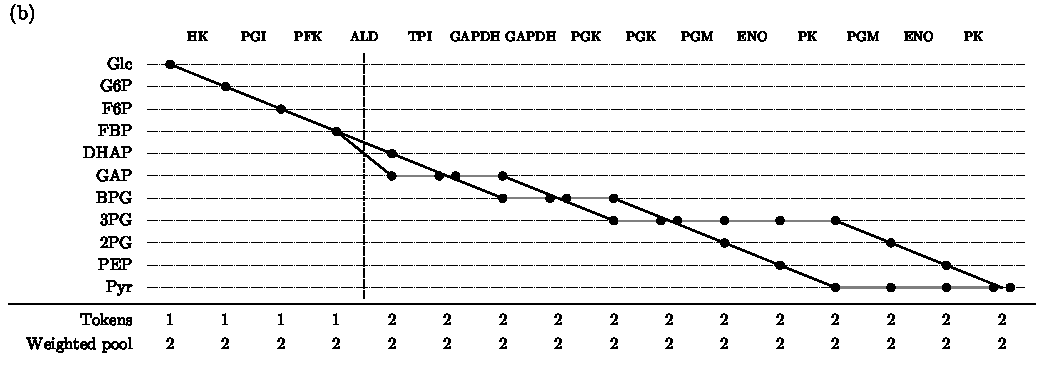
\includegraphics[width=16.4cm]{Figure/glycolysis_replay.pdf}};
\end{tikzpicture}
\endgroup
